\documentclass[12pt]{article}
\usepackage{amsmath, amssymb, amsthm}
\usepackage{array}
\usepackage{booktabs}
\usepackage[margin=1in]{geometry}
\usepackage{xcolor}
\usepackage{tcolorbox}
\tcbuselibrary{breakable}
\usepackage{enumitem}
\usepackage{fancyhdr}

\DeclareMathOperator{\logit}{logit}

% Define solution environment
\newtcolorbox{solution}{
    colback=blue!5!white,
    colframe=blue!75!black,
    title=Solution,
    fonttitle=\bfseries,
    breakable
}

\newtcolorbox{explanation}{
    colback=green!5!white,
    colframe=green!75!black,
    title=Explanation,
    fonttitle=\bfseries,
    breakable
}

\title{ASSIGNMENT 2 - SOLUTIONS}
\author{Statistical Foundation of Data Science\\
CSU1658}
\date{November 2025}

\pagestyle{fancy}
\fancyhf{}
\rhead{Assignment 2 Solutions}
\lhead{CSU1658}
\cfoot{\thepage}

\begin{document}

\maketitle

\tableofcontents
\newpage

\section{Problem 1: Zero-Inflated Normal Distribution}

\subsection{Problem Statement}
Let \( X \) be a zero-inflated normal:

\[\mathbb{P}(X = 0) = \alpha, \quad X \mid (X \neq 0) \sim \mathcal{N}(\mu, \sigma^2)\]

with prob. \((1 - \alpha)\).

\begin{enumerate}
\item Write the PMF/PDF and CDF of \( X \).
\item Derive \(\mathbb{E}[X]\) and \(\text{Var}(X)\).
\item Numerically evaluate \(\mathbb{P}(X \leq 0)\) for \(\alpha = 0.3\), \(\mu = 2\), \(\sigma = 1\).
\end{enumerate}

\subsection{Solution}

\subsubsection{Part (a): PMF/PDF and CDF of \(X\)}

\begin{solution}
A zero-inflated normal distribution is a mixture distribution that combines:
\begin{itemize}
    \item A point mass at zero with probability \(\alpha\)
    \item A normal distribution \(\mathcal{N}(\mu, \sigma^2)\) with probability \(1-\alpha\)
\end{itemize}

\textbf{Probability Density Function (PDF):}

The PDF is given by:
\[
f_X(x) = \begin{cases}
\alpha + (1-\alpha) \cdot \phi\left(\frac{x-\mu}{\sigma}\right) \cdot \frac{1}{\sigma} & \text{if } x = 0 \\
(1-\alpha) \cdot \phi\left(\frac{x-\mu}{\sigma}\right) \cdot \frac{1}{\sigma} & \text{if } x \neq 0
\end{cases}
\]

where \(\phi(z) = \frac{1}{\sqrt{2\pi}}e^{-z^2/2}\) is the standard normal PDF.

More precisely, since we have a point mass at zero, we need to be careful. The proper formulation is:

\[
\mathbb{P}(X = 0) = \alpha + (1-\alpha) \cdot f_{\mathcal{N}(\mu, \sigma^2)}(0)
\]

where \(f_{\mathcal{N}(\mu, \sigma^2)}(x) = \frac{1}{\sigma\sqrt{2\pi}} \exp\left(-\frac{(x-\mu)^2}{2\sigma^2}\right)\).

However, the standard formulation treats this as:
\begin{itemize}
    \item Point mass at 0: \(\mathbb{P}(X = 0) = \alpha\)
    \item Continuous part for \(x \neq 0\): \(f_X(x) = (1-\alpha) \cdot \frac{1}{\sigma\sqrt{2\pi}} \exp\left(-\frac{(x-\mu)^2}{2\sigma^2}\right)\)
\end{itemize}

\textbf{Cumulative Distribution Function (CDF):}

For the CDF \(F_X(x) = \mathbb{P}(X \leq x)\):

\[
F_X(x) = \begin{cases}
0 & \text{if } x < 0 \\
\alpha + (1-\alpha) \cdot \Phi\left(\frac{x-\mu}{\sigma}\right) & \text{if } x \geq 0
\end{cases}
\]

where \(\Phi(z) = \frac{1}{\sqrt{2\pi}} \int_{-\infty}^{z} e^{-t^2/2} dt\) is the standard normal CDF.
\end{solution}

\begin{explanation}
\textbf{Understanding the distribution:}

The zero-inflated normal is a \textit{mixture distribution} that arises in many real-world scenarios where:
\begin{itemize}
    \item There's a structural reason for observing exactly zero (e.g., no purchase amount, no rainfall on a given day, no claim in insurance)
    \item When non-zero values occur, they follow a normal distribution centered at \(\mu\)
\end{itemize}

\textbf{Mathematical Structure:}

The distribution can be written as a weighted mixture:
\[
X = \begin{cases}
0 & \text{with probability } \alpha \\
Y \sim \mathcal{N}(\mu, \sigma^2) & \text{with probability } (1-\alpha)
\end{cases}
\]

\textbf{PDF Analysis:}

The PDF combines a Dirac delta function at zero with a continuous normal density:
\[
f_X(x) = \alpha \cdot \delta(x) + (1-\alpha) \cdot \frac{1}{\sigma\sqrt{2\pi}} e^{-\frac{(x-\mu)^2}{2\sigma^2}}
\]

For practical purposes, we treat the point mass separately from the continuous part.

\textbf{CDF Construction:}

The CDF is built by considering three regions:

\textit{Region 1: } \(x < 0\)
\begin{itemize}
    \item No probability mass exists below zero (since we have a point mass at 0 and a normal distribution that may extend into negative values)
    \item If the normal component has \(\mu > 0\), there's still some small probability of negative values from the tail
    \item Thus: \(F_X(x) = (1-\alpha) \Phi\left(\frac{x-\mu}{\sigma}\right)\) for \(x < 0\)
\end{itemize}

\textit{Region 2: } \(x = 0\)
\begin{itemize}
    \item The CDF jumps discontinuously by amount \(\alpha\) at zero
    \item This jump represents the point mass
\end{itemize}

\textit{Region 3: } \(x > 0\)
\begin{itemize}
    \item We accumulate all probability up to \(x\):
    \item Point mass contribution: \(\alpha\)
    \item Normal component up to \(x\): \((1-\alpha) \Phi\left(\frac{x-\mu}{\sigma}\right)\)
    \item Total: \(F_X(x) = \alpha + (1-\alpha) \Phi\left(\frac{x-\mu}{\sigma}\right)\)
\end{itemize}

\textbf{Key Properties:}
\begin{enumerate}
    \item The CDF is right-continuous (follows the standard definition)
    \item At \(x = 0\): \(F_X(0) = \alpha + (1-\alpha)\Phi\left(\frac{-\mu}{\sigma}\right)\)
    \item As \(x \to \infty\): \(F_X(x) \to \alpha + (1-\alpha) \cdot 1 = 1\)
    \item As \(x \to -\infty\): \(F_X(x) \to (1-\alpha) \cdot 0 = 0\)
\end{enumerate}
\end{explanation}

\subsubsection{Part (b): Expected Value and Variance}

\begin{solution}
\textbf{Expected Value \(\mathbb{E}[X]\):}

Using the law of total expectation:
\begin{align}
\mathbb{E}[X] &= \mathbb{E}[X \mid X = 0] \cdot \mathbb{P}(X = 0) + \mathbb{E}[X \mid X \neq 0] \cdot \mathbb{P}(X \neq 0) \\
&= 0 \cdot \alpha + \mu \cdot (1-\alpha) \\
&= (1-\alpha)\mu
\end{align}

\textbf{Variance \(\text{Var}(X)\):}

We use the law of total variance:
\[
\text{Var}(X) = \mathbb{E}[\text{Var}(X \mid \text{component})] + \text{Var}(\mathbb{E}[X \mid \text{component}])
\]

Step 1: Compute \(\mathbb{E}[X^2]\)

\begin{align}
\mathbb{E}[X^2] &= \mathbb{E}[X^2 \mid X = 0] \cdot \mathbb{P}(X = 0) + \mathbb{E}[X^2 \mid X \neq 0] \cdot \mathbb{P}(X \neq 0) \\
&= 0 \cdot \alpha + \mathbb{E}[X^2 \mid X \sim \mathcal{N}(\mu, \sigma^2)] \cdot (1-\alpha)
\end{align}

For \(X \sim \mathcal{N}(\mu, \sigma^2)\):
\[
\mathbb{E}[X^2] = \text{Var}(X) + (\mathbb{E}[X])^2 = \sigma^2 + \mu^2
\]

Therefore:
\[
\mathbb{E}[X^2] = (1-\alpha)(\sigma^2 + \mu^2)
\]

Step 2: Compute variance

\begin{align}
\text{Var}(X) &= \mathbb{E}[X^2] - (\mathbb{E}[X])^2 \\
&= (1-\alpha)(\sigma^2 + \mu^2) - [(1-\alpha)\mu]^2 \\
&= (1-\alpha)(\sigma^2 + \mu^2) - (1-\alpha)^2\mu^2 \\
&= (1-\alpha)\sigma^2 + (1-\alpha)\mu^2 - (1-\alpha)^2\mu^2 \\
&= (1-\alpha)\sigma^2 + (1-\alpha)\mu^2[1 - (1-\alpha)] \\
&= (1-\alpha)\sigma^2 + (1-\alpha)\alpha\mu^2 \\
&= (1-\alpha)[\sigma^2 + \alpha\mu^2]
\end{align}

\textbf{Final Results:}
\[
\boxed{\mathbb{E}[X] = (1-\alpha)\mu}
\]
\[
\boxed{\text{Var}(X) = (1-\alpha)(\sigma^2 + \alpha\mu^2)}
\]
\end{solution}

\begin{explanation}
\textbf{Detailed Understanding:}

\textbf{1. Expected Value Derivation:}

The expectation uses the law of total expectation, conditioning on whether \(X = 0\) or not:

\begin{align*}
\mathbb{E}[X] &= \sum_{\text{all outcomes}} x \cdot \mathbb{P}(X = x) \\
&= \mathbb{E}[X \mid X = 0] \cdot \mathbb{P}(X = 0) + \mathbb{E}[X \mid X \neq 0] \cdot \mathbb{P}(X \neq 0)
\end{align*}

Breaking down each term:
\begin{itemize}
    \item \(\mathbb{E}[X \mid X = 0] = 0\) (trivially, if \(X = 0\), its expected value is 0)
    \item \(\mathbb{P}(X = 0) = \alpha\) (given in problem)
    \item \(\mathbb{E}[X \mid X \neq 0] = \mu\) (given that \(X \neq 0\), it follows \(\mathcal{N}(\mu, \sigma^2)\))
    \item \(\mathbb{P}(X \neq 0) = 1 - \alpha\) (complement of point mass probability)
\end{itemize}

Therefore: \(\mathbb{E}[X] = 0 \cdot \alpha + \mu \cdot (1-\alpha) = (1-\alpha)\mu\)

\textbf{Interpretation:} The expected value is "deflated" by the factor \((1-\alpha)\). If \(\mu = 10\) and \(\alpha = 0.3\), then \(\mathbb{E}[X] = 7\), not 10, because 30\% of the time we observe 0 instead of values near 10.

\textbf{2. Variance Derivation - Method of Moments:}

We use \(\text{Var}(X) = \mathbb{E}[X^2] - (\mathbb{E}[X])^2\).

\textit{Step 2a: Calculate \(\mathbb{E}[X^2]\)}

Using total expectation again:
\begin{align*}
\mathbb{E}[X^2] &= \mathbb{E}[X^2 \mid X = 0] \cdot \mathbb{P}(X = 0) + \mathbb{E}[X^2 \mid X \neq 0] \cdot \mathbb{P}(X \neq 0) \\
&= 0^2 \cdot \alpha + \mathbb{E}[X^2 \mid X \sim \mathcal{N}(\mu, \sigma^2)] \cdot (1-\alpha) \\
&= (1-\alpha) \cdot \mathbb{E}[Y^2]
\end{align*}

where \(Y \sim \mathcal{N}(\mu, \sigma^2)\).

For any normal random variable \(Y \sim \mathcal{N}(\mu, \sigma^2)\):
\[
\mathbb{E}[Y^2] = \text{Var}(Y) + (\mathbb{E}[Y])^2 = \sigma^2 + \mu^2
\]

This is a fundamental identity: the second moment equals variance plus squared mean.

Thus:
\[
\mathbb{E}[X^2] = (1-\alpha)(\sigma^2 + \mu^2)
\]

\textit{Step 2b: Apply Variance Formula}

\begin{align*}
\text{Var}(X) &= \mathbb{E}[X^2] - (\mathbb{E}[X])^2 \\
&= (1-\alpha)(\sigma^2 + \mu^2) - [(1-\alpha)\mu]^2 \\
&= (1-\alpha)(\sigma^2 + \mu^2) - (1-\alpha)^2\mu^2
\end{align*}

Factor out \((1-\alpha)\):
\begin{align*}
\text{Var}(X) &= (1-\alpha)[\sigma^2 + \mu^2 - (1-\alpha)\mu^2] \\
&= (1-\alpha)[\sigma^2 + \mu^2 - \mu^2 + \alpha\mu^2] \\
&= (1-\alpha)[\sigma^2 + \alpha\mu^2]
\end{align*}

\textbf{Interpretation of Variance Components:}

The variance has \textbf{two sources of variability}:

\begin{enumerate}
    \item \textbf{Inherent variability}: \((1-\alpha)\sigma^2\)
    \begin{itemize}
        \item This is the variance from the normal distribution itself
        \item Weighted by \((1-\alpha)\) because we only sample from \(\mathcal{N}(\mu, \sigma^2)\) with probability \((1-\alpha)\)
    \end{itemize}

    \item \textbf{Mixture variability}: \((1-\alpha)\alpha\mu^2\)
    \begin{itemize}
        \item This represents uncertainty about \textit{which component} we're sampling from
        \item Maximum when \(\alpha = 0.5\) (equal mixing)
        \item Increases with \(\mu^2\) (larger distance between 0 and the normal mean)
        \item Vanishes when \(\alpha = 0\) (no inflation) or \(\alpha = 1\) (always zero)
    \end{itemize}
\end{enumerate}

\textbf{Limiting Cases Verification:}
\begin{itemize}
    \item If \(\alpha = 0\) (no inflation): \(\text{Var}(X) = \sigma^2\)  (pure normal)
    \item If \(\alpha = 1\) (always zero): \(\text{Var}(X) = 0\)  (degenerate)
    \item If \(\mu = 0\): \(\text{Var}(X) = (1-\alpha)\sigma^2\) (reduced variance due to mixing with zero)
\end{itemize}
\end{explanation}

\subsubsection{Part (c): Numerical Evaluation}

\begin{solution}
Given: \(\alpha = 0.3\), \(\mu = 2\), \(\sigma = 1\)

We need to find \(\mathbb{P}(X \leq 0)\).

Since the zero-inflated normal has a point mass at 0 and is continuous elsewhere:

\[
\mathbb{P}(X \leq 0) = \mathbb{P}(X = 0) + \mathbb{P}(0 < X \leq 0)
\]

The second term is zero (no interval), so we need:

\[
\mathbb{P}(X \leq 0) = \mathbb{P}(X = 0) + \mathbb{P}(X < 0)
\]

\textbf{Step 1: Probability of exactly zero}
\[
\mathbb{P}(X = 0) = \alpha = 0.3
\]

\textbf{Step 2: Probability of negative values}

The negative values can only come from the normal component:
\begin{align}
\mathbb{P}(X < 0) &= (1-\alpha) \cdot \mathbb{P}(\mathcal{N}(\mu, \sigma^2) < 0) \\
&= (1-\alpha) \cdot \Phi\left(\frac{0-\mu}{\sigma}\right) \\
&= 0.7 \cdot \Phi\left(\frac{-2}{1}\right) \\
&= 0.7 \cdot \Phi(-2)
\end{align}

From standard normal tables: \(\Phi(-2) \approx 0.0228\)

Therefore:
\[
\mathbb{P}(X < 0) = 0.7 \times 0.0228 = 0.01596
\]

\textbf{Step 3: Total probability}
\begin{align}
\mathbb{P}(X \leq 0) &= \mathbb{P}(X = 0) + \mathbb{P}(X < 0) \\
&= 0.3 + 0.01596 \\
&= 0.31596
\end{align}

\[
\boxed{\mathbb{P}(X \leq 0) \approx 0.316 \text{ or } 31.6\%}
\]

\textbf{Verification using exact value:}

More precisely, \(\Phi(-2) = 0.02275013...\), so:
\[
\mathbb{P}(X \leq 0) = 0.3 + 0.7(0.02275013) = 0.3 + 0.01592509 = 0.31592509 \approx \boxed{0.3159}
\]
\end{solution}

\begin{explanation}
\textbf{Detailed Numerical Computation:}

\textbf{Step-by-Step Breakdown:}

We need to find \(\mathbb{P}(X \leq 0)\), which includes all probability mass at or below zero.

\textit{Understanding the Event \(\{X \leq 0\}\):}

This event can be partitioned into two disjoint cases:
\begin{enumerate}
    \item \(X = 0\) exactly (the point mass)
    \item \(X < 0\) (negative values from the normal tail)
\end{enumerate}

Therefore: \(\mathbb{P}(X \leq 0) = \mathbb{P}(X = 0) + \mathbb{P}(X < 0)\)

\textbf{Part 1: Point Mass at Zero}

By definition of the zero-inflated distribution:
\[
\mathbb{P}(X = 0) = \alpha = 0.3
\]

This is the structural zero component - 30\% of observations are exactly zero by design.

\textbf{Part 2: Negative Values from Normal Component}

Negative values can \textit{only} arise from the normal component, and only when that component is sampled (which happens with probability \(1-\alpha\)).

Using the law of total probability:
\begin{align*}
\mathbb{P}(X < 0) &= \mathbb{P}(X < 0 \mid \text{sample from normal}) \cdot \mathbb{P}(\text{sample from normal}) \\
&\quad + \mathbb{P}(X < 0 \mid X = 0) \cdot \mathbb{P}(X = 0) \\
&= \mathbb{P}(\mathcal{N}(\mu, \sigma^2) < 0) \cdot (1-\alpha) + 0 \cdot \alpha \\
&= (1-\alpha) \cdot \mathbb{P}(Y < 0)
\end{align*}

where \(Y \sim \mathcal{N}(\mu, \sigma^2) = \mathcal{N}(2, 1)\).

\textit{Standardization Process:}

To evaluate \(\mathbb{P}(Y < 0)\), we standardize:
\begin{align*}
\mathbb{P}(Y < 0) &= \mathbb{P}\left(\frac{Y - \mu}{\sigma} < \frac{0 - \mu}{\sigma}\right) \\
&= \mathbb{P}\left(Z < \frac{0 - 2}{1}\right) \quad \text{where } Z \sim \mathcal{N}(0, 1) \\
&= \mathbb{P}(Z < -2) \\
&= \Phi(-2)
\end{align*}

\textit{Standard Normal Table Lookup:}

From the standard normal distribution table (or using symmetry):
\begin{align*}
\Phi(-2) &= 1 - \Phi(2) \quad \text{(by symmetry of normal distribution)} \\
&= 1 - 0.9772 \\
&= 0.0228
\end{align*}

More precisely: \(\Phi(-2) = 0.02275013...\)

\textbf{Physical Interpretation:} Even though the normal distribution is centered at \(\mu = 2\) (well above zero), there's still a small probability (2.28\%) that a sample from it will be negative, due to the left tail extending to \(-\infty\).

The value \(x = 0\) is exactly \(\frac{0-2}{1} = -2\) standard deviations below the mean.

\textit{Computing Probability from Normal Component:}
\begin{align*}
\mathbb{P}(X < 0) &= (1-\alpha) \cdot \Phi(-2) \\
&= 0.7 \times 0.0228 \\
&= 0.01596
\end{align*}

\textbf{Part 3: Total Probability}

Combining both sources:
\begin{align*}
\mathbb{P}(X \leq 0) &= \underbrace{0.3}_{\text{point mass}} + \underbrace{0.01596}_{\text{normal tail}} \\
&= 0.31596 \\
&\approx 0.316
\end{align*}

\textbf{Using More Precise Values:}

With \(\Phi(-2) = 0.02275013194817921\):
\begin{align*}
\mathbb{P}(X < 0) &= 0.7 \times 0.02275013 = 0.015925092 \\
\mathbb{P}(X \leq 0) &= 0.3 + 0.015925092 = 0.315925092 \\
&\approx \boxed{0.3159}
\end{align*}

\textbf{Verification by CDF Formula:}

We can verify using our CDF from part (a):
\begin{align*}
F_X(0) &= \alpha + (1-\alpha) \Phi\left(\frac{0-\mu}{\sigma}\right) \\
&= 0.3 + 0.7 \times \Phi(-2) \\
&= 0.3 + 0.7 \times 0.0228 \\
&= 0.3159 \quad \text{(verified)}
\end{align*}

\textbf{Final Interpretation:}

Out of a large sample:
\begin{itemize}
    \item Approximately \textbf{30.0\%} will be exactly zero (structural zeros)
    \item Approximately \textbf{1.6\%} will be negative (from normal tail)
    \item Approximately \textbf{68.4\%} will be positive (from normal component above zero)
\end{itemize}

The vast majority of the "at or below zero" probability (94.9\%) comes from the point mass itself, with only a small contribution (5.1\%) from the negative tail of the normal distribution.

\textbf{Sensitivity Analysis:}

If we changed parameters:
\begin{itemize}
    \item Larger \(\mu\): \(\Phi\left(\frac{-\mu}{\sigma}\right)\) decreases, so \(\mathbb{P}(X < 0)\) decreases
    \item Larger \(\sigma\): More spread, so \(\mathbb{P}(X < 0)\) increases (thicker tails)
    \item Larger \(\alpha\): More point mass, so \(\mathbb{P}(X \leq 0)\) increases linearly
\end{itemize}
\end{explanation}

\newpage

\section{Problem 2: Binomial Distribution and Normal Approximation}

\subsection{Problem Statement}
Let \( X \sim \text{Bin}(n, p) \) with \( n = 10, \, p = 0.3 \).
\begin{enumerate}
\item Compute exactly \(\mathbb{P}(X \geq 6)\).
\item Approximate \(\mathbb{P}(X \geq 6)\) by a normal approximation with continuity correction and compare.
\end{enumerate}

\subsection{Solution}

\subsubsection{Part (a): Exact Binomial Probability}

\begin{solution}
For \(X \sim \text{Bin}(n, p)\) with \(n = 10\) and \(p = 0.3\), we need \(\mathbb{P}(X \geq 6)\).

\textbf{Binomial PMF:}

The probability mass function is:
\[
\mathbb{P}(X = k) = \binom{n}{k} p^k (1-p)^{n-k} = \binom{10}{k} (0.3)^k (0.7)^{10-k}
\]

\textbf{Computing the Tail Probability:}

Using the complement rule:
\begin{align*}
\mathbb{P}(X \geq 6) &= 1 - \mathbb{P}(X \leq 5) \\
&= \mathbb{P}(X = 6) + \mathbb{P}(X = 7) + \mathbb{P}(X = 8) + \mathbb{P}(X = 9) + \mathbb{P}(X = 10)
\end{align*}

We'll compute each term directly.

\textbf{Computing Each Probability:}

\textit{For \(k = 6\):}
\begin{align*}
\mathbb{P}(X = 6) &= \binom{10}{6} (0.3)^6 (0.7)^4 \\
&= \frac{10!}{6! \cdot 4!} \times (0.3)^6 \times (0.7)^4 \\
&= 210 \times 0.000729 \times 0.2401 \\
&= 210 \times 0.000175 \\
&= 0.036757
\end{align*}

\textit{For \(k = 7\):}
\begin{align*}
\mathbb{P}(X = 7) &= \binom{10}{7} (0.3)^7 (0.7)^3 \\
&= 120 \times 0.0002187 \times 0.343 \\
&= 120 \times 0.0000750141 \\
&= 0.009002
\end{align*}

\textit{For \(k = 8\):}
\begin{align*}
\mathbb{P}(X = 8) &= \binom{10}{8} (0.3)^8 (0.7)^2 \\
&= 45 \times 0.00006561 \times 0.49 \\
&= 45 \times 0.000032149 \\
&= 0.001447
\end{align*}

\textit{For \(k = 9\):}
\begin{align*}
\mathbb{P}(X = 9) &= \binom{10}{9} (0.3)^9 (0.7)^1 \\
&= 10 \times 0.000019683 \times 0.7 \\
&= 10 \times 0.0000137781 \\
&= 0.000138
\end{align*}

\textit{For \(k = 10\):}
\begin{align*}
\mathbb{P}(X = 10) &= \binom{10}{10} (0.3)^{10} (0.7)^0 \\
&= 1 \times 0.0000059049 \times 1 \\
&= 0.0000059
\end{align*}

\textbf{Summing the Probabilities:}
\begin{align*}
\mathbb{P}(X \geq 6) &= 0.036757 + 0.009002 + 0.001447 + 0.000138 + 0.0000059 \\
&= 0.0473499 \\
&\approx \boxed{0.0473}
\end{align*}

More precisely: \(\mathbb{P}(X \geq 6) = 0.047349\)
\end{solution}

\begin{explanation}
\textbf{Understanding the Calculation:}

\begin{itemize}
    \item With \(n = 10\) trials and success probability \(p = 0.3\), the expected number of successes is \(\mathbb{E}[X] = np = 3\).

    \item We're looking for the probability of getting 6 or more successes, which is \textbf{far in the right tail} of this distribution (about 3 standard deviations above the mean).

    \item The binomial coefficient \(\binom{10}{k}\) counts the number of ways to arrange \(k\) successes in 10 trials:
    \begin{itemize}
        \item \(\binom{10}{6} = 210\) ways
        \item \(\binom{10}{7} = 120\) ways
        \item \(\binom{10}{8} = 45\) ways
        \item \(\binom{10}{9} = 10\) ways
        \item \(\binom{10}{10} = 1\) way
    \end{itemize}

    \item Even though there are many ways to get 6 successes (210), each specific sequence has very low probability: \((0.3)^6(0.7)^4 \approx 0.000175\).

    \item The probabilities decrease rapidly as \(k\) increases because:
    \begin{enumerate}
        \item Each additional success multiplies by 0.3
        \item Each fewer failure divides by 0.7
        \item The ratio \(\frac{p}{1-p} = \frac{0.3}{0.7} \approx 0.43 < 1\) makes higher values exponentially less likely
    \end{enumerate}

    \item \textbf{Interpretation:} Getting 6 or more successes when \(p = 0.3\) happens only about 4.7\% of the time - this is a relatively rare event.
\end{itemize}
\end{explanation}

\subsubsection{Part (b): Normal Approximation with Continuity Correction}

\begin{solution}
\textbf{Normal Approximation to Binomial:}

For large \(n\), the binomial distribution \(\text{Bin}(n, p)\) can be approximated by a normal distribution with:
\begin{align*}
\mu &= np = 10 \times 0.3 = 3 \\
\sigma^2 &= np(1-p) = 10 \times 0.3 \times 0.7 = 2.1 \\
\sigma &= \sqrt{2.1} = 1.449
\end{align*}

So \(X \approx \mathcal{N}(3, 2.1)\).

\textbf{Continuity Correction:}

Since we're approximating a discrete distribution (integer values) with a continuous one, we need a continuity correction.

For \(\mathbb{P}(X \geq 6)\) where \(X\) is discrete, we want the probability that the continuous approximation exceeds 5.5 (the midpoint between 5 and 6):

\[
\mathbb{P}(X \geq 6) \approx \mathbb{P}(Y > 5.5)
\]

where \(Y \sim \mathcal{N}(3, 2.1)\).

\textbf{Standardization:}

Convert to standard normal:
\begin{align*}
\mathbb{P}(Y > 5.5) &= \mathbb{P}\left(\frac{Y - \mu}{\sigma} > \frac{5.5 - \mu}{\sigma}\right) \\
&= \mathbb{P}\left(Z > \frac{5.5 - 3}{1.449}\right) \\
&= \mathbb{P}\left(Z > \frac{2.5}{1.449}\right) \\
&= \mathbb{P}(Z > 1.726)
\end{align*}

where \(Z \sim \mathcal{N}(0, 1)\).

\textbf{Using Standard Normal Table:}

From the standard normal table:
\begin{align*}
\Phi(1.726) &\approx \Phi(1.73) \approx 0.9582
\end{align*}

Therefore:
\begin{align*}
\mathbb{P}(Z > 1.726) &= 1 - \Phi(1.726) \\
&= 1 - 0.9582 \\
&= 0.0418
\end{align*}

\[
\boxed{\mathbb{P}(X \geq 6) \approx 0.0418 \text{ (normal approximation)}}
\]

\textbf{Comparison with Exact Value:}

\begin{center}
\begin{tabular}{lcc}
\toprule
Method & Probability & Error \\
\midrule
Exact Binomial & 0.0473 & --- \\
Normal Approximation (with CC) & 0.0418 & 0.0055 \\
Relative Error & --- & 11.6\% \\
\bottomrule
\end{tabular}
\end{center}

The normal approximation \textbf{underestimates} the true probability by about 0.0055 (or 11.6\% relative error).
\end{solution}

\begin{explanation}
\textbf{Detailed Analysis:}

\textbf{1. Why Use Normal Approximation?}

The Central Limit Theorem tells us that sums of independent random variables (which the binomial is) approach normality. Specifically, for \(X \sim \text{Bin}(n, p)\):
\[
\frac{X - np}{\sqrt{np(1-p)}} \xrightarrow{d} \mathcal{N}(0, 1) \text{ as } n \to \infty
\]

\textbf{2. Rule of Thumb for Approximation Quality:}

The normal approximation works well when:
\begin{itemize}
    \item \(np \geq 5\) and \(n(1-p) \geq 5\)
    \item In our case: \(np = 3\) and \(n(1-p) = 7\)
    \item Since \(np = 3 < 5\), the approximation may not be very accurate!
\end{itemize}

This explains why our approximation has a relatively large error (11.6\%).

\textbf{3. Continuity Correction Explained:}

The continuity correction accounts for the fact that:
\begin{itemize}
    \item Discrete \(X\): takes values \(\{0, 1, 2, \ldots, 10\}\)
    \item Continuous \(Y\): takes any real value
\end{itemize}

For \(\mathbb{P}(X \geq 6)\), we're including the bar from 5.5 to 6.5 in the histogram, so we approximate:
\[
\mathbb{P}(X \geq 6) \approx \mathbb{P}(Y \geq 5.5)
\]

\textbf{Visual interpretation:} Imagine the binomial as a histogram with bars centered at integers. The normal curve should approximate the area under those bars. The value 5.5 is the left edge of the bar at 6.

\textbf{4. Direction of Error:}

The normal approximation gave 0.0418 vs. exact 0.0473:
\begin{itemize}
    \item The approximation underestimated by 11.6\%
    \item This is expected because:
    \begin{enumerate}
        \item Small sample size (\(n = 10\))
        \item \(p = 0.3\) creates right skewness in the binomial
        \item Normal distribution is symmetric, missing the tail behavior
        \item We're evaluating far from the mean (6 vs. 3)
    \end{enumerate}
\end{itemize}

\textbf{5. Standardization Steps:}

The z-score calculation:
\[
z = \frac{5.5 - 3}{1.449} = \frac{2.5}{1.449} = 1.726
\]

This tells us that 5.5 is 1.726 standard deviations above the mean. Since \(\Phi(1.726) = 0.9582\), about 95.82\% of the normal distribution is below this value, leaving 4.18\% above.

\textbf{6. When Would the Approximation Be Better?}

If we had:
\begin{itemize}
    \item \(n = 100, p = 0.3\): \(np = 30 \geq 5\) and \(n(1-p) = 70 \geq 5\)
    \item The approximation would be much more accurate
    \item Relative error would typically be under 1\%
\end{itemize}

\textbf{Conclusion:} While the normal approximation is computationally simpler (no need to sum multiple binomial probabilities), it should be used cautiously when \(n\) is small or \(p\) is far from 0.5. In this case, the 11.6\% error is significant, and the exact calculation is preferred.
\end{explanation}

\newpage

\section{Problem 3: Poisson Thinning Property}

\subsection{Problem Statement}
Suppose \( N \sim \text{Poisson}(\lambda) \). Conditional on \( N \), each of the \( N \) events is independently tagged "A" with probability \( q \) (and "B" otherwise). Let \( K \) be the number of "A" events.
\begin{enumerate}
\item Show \( K \sim \text{Poisson}(\lambda q) \) (the thinning property).
\item Show that, conditional on \( N = n, \, K \mid N = n \sim \text{Bin}(n, q) \).
\item For \( \lambda = 12, \, q = 0.2 \), compute \(\mathbb{P}(K = 0)\) and \(\mathbb{P}(K \leq 2)\) exactly (closed form).
\end{enumerate}

\subsection{Solution}

\subsubsection{Part (a): Thinning Property - Showing \(K \sim \text{Poisson}(\lambda q)\)}

\begin{solution}
We need to prove that \(K\), the number of "A" events, follows a Poisson distribution with parameter \(\lambda q\).

\textbf{Strategy:} Use the law of total probability by conditioning on \(N\).

\textbf{Step 1: Set up the conditional structure}

Given \(N = n\), we have \(n\) events, and each is independently tagged "A" with probability \(q\). Therefore:
\[
K \mid N = n \sim \text{Bin}(n, q)
\]

This means:
\[
\mathbb{P}(K = k \mid N = n) = \binom{n}{k} q^k (1-q)^{n-k} \quad \text{for } k \leq n
\]

\textbf{Step 2: Apply law of total probability}

To find the unconditional distribution of \(K\), we sum over all possible values of \(N\):
\begin{align*}
\mathbb{P}(K = k) &= \sum_{n=0}^{\infty} \mathbb{P}(K = k \mid N = n) \cdot \mathbb{P}(N = n)
\end{align*}

Note that \(\mathbb{P}(K = k \mid N = n) = 0\) when \(n < k\), so:
\begin{align*}
\mathbb{P}(K = k) &= \sum_{n=k}^{\infty} \mathbb{P}(K = k \mid N = n) \cdot \mathbb{P}(N = n)
\end{align*}

\textbf{Step 3: Substitute the distributions}

Since \(N \sim \text{Poisson}(\lambda)\):
\[
\mathbb{P}(N = n) = \frac{\lambda^n e^{-\lambda}}{n!}
\]

Substituting both distributions:
\begin{align*}
\mathbb{P}(K = k) &= \sum_{n=k}^{\infty} \binom{n}{k} q^k (1-q)^{n-k} \cdot \frac{\lambda^n e^{-\lambda}}{n!}
\end{align*}

\textbf{Step 4: Simplify the binomial coefficient}

Recall: \(\binom{n}{k} = \frac{n!}{k!(n-k)!}\)

\begin{align*}
\mathbb{P}(K = k) &= \sum_{n=k}^{\infty} \frac{n!}{k!(n-k)!} q^k (1-q)^{n-k} \cdot \frac{\lambda^n e^{-\lambda}}{n!} \\
&= \sum_{n=k}^{\infty} \frac{q^k (1-q)^{n-k} \lambda^n e^{-\lambda}}{k!(n-k)!} \\
&= \frac{q^k e^{-\lambda}}{k!} \sum_{n=k}^{\infty} \frac{\lambda^n (1-q)^{n-k}}{(n-k)!}
\end{align*}

\textbf{Step 5: Change of variables}

Let \(m = n - k\), so \(n = m + k\). When \(n = k\), \(m = 0\); when \(n \to \infty\), \(m \to \infty\):

\begin{align*}
\mathbb{P}(K = k) &= \frac{q^k e^{-\lambda}}{k!} \sum_{m=0}^{\infty} \frac{\lambda^{m+k} (1-q)^{m}}{m!} \\
&= \frac{q^k \lambda^k e^{-\lambda}}{k!} \sum_{m=0}^{\infty} \frac{[\lambda(1-q)]^{m}}{m!}
\end{align*}

\textbf{Step 6: Recognize the exponential series}

The sum \(\sum_{m=0}^{\infty} \frac{x^m}{m!} = e^x\), so:
\begin{align*}
\sum_{m=0}^{\infty} \frac{[\lambda(1-q)]^{m}}{m!} = e^{\lambda(1-q)}
\end{align*}

\textbf{Step 7: Final simplification}

\begin{align*}
\mathbb{P}(K = k) &= \frac{q^k \lambda^k e^{-\lambda}}{k!} \cdot e^{\lambda(1-q)} \\
&= \frac{(\lambda q)^k}{k!} \cdot e^{-\lambda} \cdot e^{\lambda(1-q)} \\
&= \frac{(\lambda q)^k}{k!} \cdot e^{-\lambda + \lambda(1-q)} \\
&= \frac{(\lambda q)^k}{k!} \cdot e^{-\lambda + \lambda - \lambda q} \\
&= \frac{(\lambda q)^k}{k!} \cdot e^{-\lambda q}
\end{align*}

\textbf{Conclusion:}

This is exactly the PMF of a Poisson distribution with parameter \(\lambda q\):
\[
\boxed{K \sim \text{Poisson}(\lambda q)}
\]
\end{solution}

\begin{explanation}
\textbf{Understanding Poisson Thinning:}

The thinning property is a fundamental result in probability theory with important practical applications.

\textbf{Intuitive Explanation:}

Imagine events arriving according to a Poisson process with rate \(\lambda\) (e.g., customers arriving at a store). Each customer is randomly classified as type "A" with probability \(q\) (e.g., paying customers) or type "B" with probability \(1-q\) (e.g., browsers).

The theorem states that:
\begin{itemize}
    \item Type A customers \textit{also} arrive as a Poisson process, but with rate \(\lambda q\)
    \item Type B customers arrive as a Poisson process with rate \(\lambda(1-q)\)
    \item These two processes are \textbf{independent}
\end{itemize}

\textbf{Why This Works:}

The key steps in the proof were:
\begin{enumerate}
    \item \textbf{Conditioning:} Given \(N = n\) total events, the number of "A" events follows \(\text{Bin}(n, q)\)

    \item \textbf{Marginalization:} We summed over all possible values of \(N\) using the law of total probability

    \item \textbf{Algebraic magic:} The binomial-Poisson convolution simplified beautifully because:
    \[
    e^{-\lambda} \cdot e^{\lambda(1-q)} = e^{-\lambda q}
    \]

    \item \textbf{Result:} All the \((1-q)\) terms got absorbed into the exponential, leaving us with \(\lambda q\)
\end{enumerate}

\textbf{Practical Applications:}

\begin{itemize}
    \item \textbf{Telecommunications:} Packets arriving at a router (Poisson) are routed to different destinations with various probabilities

    \item \textbf{Queueing Theory:} Customers arriving at a service center may choose different service types

    \item \textbf{Particle Physics:} Radioactive decay events can produce different types of particles

    \item \textbf{Insurance:} Claims arriving at an insurance company can be classified by type
\end{itemize}

\textbf{Important Note:} This property is \textbf{unique to the Poisson distribution}. If events arrived according to a binomial or any other distribution, thinning would \textit{not} preserve the distribution type.
\end{explanation}

\subsubsection{Part (b): Conditional Distribution}

\begin{solution}
We need to show that \(K \mid N = n \sim \text{Bin}(n, q)\).

\textbf{Setup:}

Given that \(N = n\) (we observe exactly \(n\) events), each event is independently tagged "A" with probability \(q\) and "B" with probability \(1-q\).

\textbf{Derivation:}

Let's denote the \(i\)-th event as \(X_i\), where:
\[
X_i = \begin{cases}
1 & \text{if event } i \text{ is tagged "A"} \\
0 & \text{if event } i \text{ is tagged "B"}
\end{cases}
\]

Each \(X_i\) is a Bernoulli random variable with:
\[
\mathbb{P}(X_i = 1) = q, \quad \mathbb{P}(X_i = 0) = 1-q
\]

Given \(N = n\), the total number of "A" events is:
\[
K = \sum_{i=1}^{n} X_i
\]

Since the \(X_i\)'s are independent Bernoulli trials with success probability \(q\), their sum follows a binomial distribution:

\[
\boxed{K \mid N = n \sim \text{Bin}(n, q)}
\]

\textbf{Explicit PMF:}

For \(k \in \{0, 1, 2, \ldots, n\}\):
\[
\mathbb{P}(K = k \mid N = n) = \binom{n}{k} q^k (1-q)^{n-k}
\]

This represents:
\begin{itemize}
    \item \(\binom{n}{k}\): number of ways to choose which \(k\) events are tagged "A"
    \item \(q^k\): probability that those \(k\) events are all "A"
    \item \((1-q)^{n-k}\): probability that the remaining \(n-k\) events are all "B"
\end{itemize}
\end{solution}

\begin{explanation}
\textbf{Conceptual Understanding:}

This result is more straightforward than part (a), but it's crucial for understanding the overall structure.

\textbf{The Two-Level Randomness:}

The problem has two sources of randomness:
\begin{enumerate}
    \item \textbf{First level (unconditional):} The number of events \(N\) is random, following \(\text{Poisson}(\lambda)\)

    \item \textbf{Second level (conditional):} Given \(N = n\), each event is randomly classified
\end{enumerate}

\textbf{Connection to Part (a):}

Part (b) gives us \(\mathbb{P}(K = k \mid N = n)\), which we then used in part (a) to derive the unconditional distribution of \(K\):

\[
\mathbb{P}(K = k) = \sum_{n=k}^{\infty} \underbrace{\mathbb{P}(K = k \mid N = n)}_{\text{Part (b)}} \cdot \underbrace{\mathbb{P}(N = n)}_{\text{Poisson}}
\]

\textbf{Interpretation:}

If someone tells you "there were exactly 10 events today," and you know each event is tagged "A" with probability 0.3, then the number of "A" events follows \(\text{Bin}(10, 0.3)\) - exactly like flipping 10 coins, each with heads probability 0.3.

The Poisson nature of \(N\) doesn't matter once we condition on its value!

\textbf{Verification:}

We can verify consistency:
\begin{align*}
\mathbb{E}[K \mid N = n] &= nq \\
\mathbb{E}[K] &= \mathbb{E}[\mathbb{E}[K \mid N]] = \mathbb{E}[Nq] = q\mathbb{E}[N] = q\lambda
\end{align*}

This matches the mean of \(\text{Poisson}(\lambda q)\):
\end{explanation}

\subsubsection{Part (c): Numerical Evaluation}

\begin{solution}
Given: \(\lambda = 12\), \(q = 0.2\)

From part (a), we know \(K \sim \text{Poisson}(\lambda q) = \text{Poisson}(12 \times 0.2) = \text{Poisson}(2.4)\).

The PMF of a Poisson distribution is:
\[
\mathbb{P}(K = k) = \frac{(\lambda q)^k e^{-\lambda q}}{k!} = \frac{(2.4)^k e^{-2.4}}{k!}
\]

\textbf{Computing \(\mathbb{P}(K = 0)\):}

\begin{align*}
\mathbb{P}(K = 0) &= \frac{(2.4)^0 e^{-2.4}}{0!} \\
&= \frac{1 \cdot e^{-2.4}}{1} \\
&= e^{-2.4} \\
&= 0.0907... \\
&\approx \boxed{0.0907}
\end{align*}

\textbf{Computing \(\mathbb{P}(K \leq 2)\):}

\begin{align*}
\mathbb{P}(K \leq 2) &= \mathbb{P}(K = 0) + \mathbb{P}(K = 1) + \mathbb{P}(K = 2)
\end{align*}

\textit{For \(k = 1\):}
\begin{align*}
\mathbb{P}(K = 1) &= \frac{(2.4)^1 e^{-2.4}}{1!} \\
&= 2.4 \cdot e^{-2.4} \\
&= 2.4 \times 0.0907... \\
&= 0.2177
\end{align*}

\textit{For \(k = 2\):}
\begin{align*}
\mathbb{P}(K = 2) &= \frac{(2.4)^2 e^{-2.4}}{2!} \\
&= \frac{5.76 \cdot e^{-2.4}}{2} \\
&= 2.88 \times 0.0907... \\
&= 0.2613
\end{align*}

\textbf{Total:}
\begin{align*}
\mathbb{P}(K \leq 2) &= 0.0907 + 0.2177 + 0.2613 \\
&= 0.5697 \\
&\approx \boxed{0.570}
\end{align*}

\textbf{Summary in Closed Form:}

\[
\boxed{\mathbb{P}(K = 0) = e^{-2.4} \approx 0.0907}
\]

\[
\boxed{\mathbb{P}(K \leq 2) = e^{-2.4}\left(1 + 2.4 + \frac{(2.4)^2}{2}\right) = e^{-2.4}(1 + 2.4 + 2.88) = 6.28 e^{-2.4} \approx 0.570}
\]
\end{solution}

\begin{explanation}
\textbf{Numerical Interpretation:}

\textbf{Context:} We start with an average of \(\lambda = 12\) events, and each event is tagged "A" with probability \(q = 0.2\).

\textbf{Expected number of "A" events:} \(\lambda q = 2.4\)

\textbf{Results Analysis:}

\begin{enumerate}
    \item \textbf{\(\mathbb{P}(K = 0) = 0.0907\):}
    \begin{itemize}
        \item About 9.1\% chance of observing zero "A" events
        \item Even though we expect 2.4 "A" events on average, there's still a non-negligible chance of getting none
        \item This makes sense: with only 20\% tagging probability, it's possible (though unlikely) that all events are tagged "B"
    \end{itemize}

    \item \textbf{\(\mathbb{P}(K \leq 2) = 0.570\):}
    \begin{itemize}
        \item About 57\% chance of observing 2 or fewer "A" events
        \item Since the mean is 2.4, it's reasonable that the probability of being at or below 2 is close to 50\%
        \item The distribution is slightly right-skewed (mean = 2.4 > median $\approx$ 2)
    \end{itemize}
\end{enumerate}

\textbf{Verification Using Expected Value:}

\begin{align*}
\mathbb{E}[K] &= \lambda q = 12 \times 0.2 = 2.4 \\
\text{Var}(K) &= \lambda q = 2.4 \quad \text{(for Poisson)} \\
\sigma_K &= \sqrt{2.4} = 1.549
\end{align*}

So \(K = 0\) is about \(\frac{0 - 2.4}{1.549} = -1.55\) standard deviations below the mean, which corresponds to roughly the 6th percentile - close to our calculated 9.1\%.

\textbf{Comparison with Direct Calculation:}

We could have computed this by summing over all \(N\):
\[
\mathbb{P}(K = 0) = \sum_{n=0}^{\infty} \mathbb{P}(K = 0 \mid N = n) \mathbb{P}(N = n)
\]

But thanks to the thinning property, we get the simple closed form \(e^{-2.4}\) directly!

\textbf{Practical Example:}

If this represented:
\begin{itemize}
    \item 12 customers arriving at a store on average (Poisson)
    \item Each makes a purchase with probability 0.2
    \item Then we'd expect 2.4 purchases on average
    \item 9.1\% of days would have zero purchases
    \item 57\% of days would have 2 or fewer purchases
\end{itemize}
\end{explanation}

\section{Problem 4: Data Standardization and Scaling}

\textbf{Problem Statement:} Let \(X=(X_{1},\ldots,X_{n})\) be nonconstant real data with population mean \(\mu=\frac{1}{n}\sum_{i}X_{i}\) and population standard deviation \(\sigma=\sqrt{\frac{1}{n}\sum_{i}(X_{i}-\mu)^{2}}\). Define:
\begin{itemize}
\item \textbf{z-score standardization:} \(Z_{i}=\frac{X_{i}-\mu}{\sigma}\)
\item \textbf{min-max normalization to \([0,1]\):} \(M_{i}=\frac{X_{i}-\min X}{\max X-\min X}\)
\item \textbf{robust scaling (median/IQR):} \(R_{i}=\frac{X_{i}-\mathrm{med}(X)}{\mathrm{IQR}(X)}\)
\end{itemize}

\subsection{Part (a): Prove that \(\bar{Z}=0\) and \(\text{Var}(Z)=1\)}

\begin{solution}
We need to prove two properties of z-score standardization.

\textbf{Property 1: The mean of z-scores is zero.}

\begin{align*}
\bar{Z} &= \frac{1}{n}\sum_{i=1}^{n} Z_i \\
&= \frac{1}{n}\sum_{i=1}^{n} \frac{X_i - \mu}{\sigma} \\
&= \frac{1}{\sigma} \cdot \frac{1}{n}\sum_{i=1}^{n} (X_i - \mu) \\
&= \frac{1}{\sigma} \left(\frac{1}{n}\sum_{i=1}^{n} X_i - \frac{1}{n}\sum_{i=1}^{n} \mu\right) \\
&= \frac{1}{\sigma} \left(\mu - \mu\right) \\
&= \frac{0}{\sigma} = 0
\end{align*}

\textbf{Property 2: The variance of z-scores is one.}

Using the definition of population variance:
\begin{align*}
\text{Var}(Z) &= \frac{1}{n}\sum_{i=1}^{n} (Z_i - \bar{Z})^2 \\
&= \frac{1}{n}\sum_{i=1}^{n} (Z_i - 0)^2 \quad \text{(since } \bar{Z} = 0\text{)} \\
&= \frac{1}{n}\sum_{i=1}^{n} Z_i^2 \\
&= \frac{1}{n}\sum_{i=1}^{n} \left(\frac{X_i - \mu}{\sigma}\right)^2 \\
&= \frac{1}{n}\sum_{i=1}^{n} \frac{(X_i - \mu)^2}{\sigma^2} \\
&= \frac{1}{\sigma^2} \cdot \frac{1}{n}\sum_{i=1}^{n} (X_i - \mu)^2 \\
&= \frac{1}{\sigma^2} \cdot \sigma^2 \quad \text{(by definition of } \sigma^2\text{)} \\
&= 1
\end{align*}

Therefore, we have proven both properties:
\[
\boxed{\bar{Z} = 0 \quad \text{and} \quad \text{Var}(Z) = 1}
\]
\end{solution}

\begin{explanation}
\textbf{Why This Matters:}

The z-score transformation is a \textbf{location-scale standardization} that:
\begin{itemize}
    \item \textbf{Centers the data:} Subtracting \(\mu\) shifts the distribution to have mean 0
    \item \textbf{Scales to unit variance:} Dividing by \(\sigma\) rescales so the spread is standardized
    \item \textbf{Preserves shape:} The distribution's shape (skewness, kurtosis) is unchanged
    \item \textbf{Makes comparisons possible:} Variables with different units/scales become comparable
\end{itemize}

\textbf{Key Algebraic Techniques:}
\begin{enumerate}
    \item \textbf{Linearity of summation:} \(\sum(aX_i + b) = a\sum X_i + nb\)
    \item \textbf{Definition exploitation:} We used \(\mu = \frac{1}{n}\sum X_i\) and \(\sigma^2 = \frac{1}{n}\sum(X_i-\mu)^2\)
    \item \textbf{Substitution strategy:} Express everything in terms of the original data moments
\end{enumerate}

\textbf{Interpretation of Results:}
\begin{itemize}
    \item A z-score of 0 means "at the mean"
    \item A z-score of +1 means "one standard deviation above the mean"
    \item A z-score of -2 means "two standard deviations below the mean"
    \item About 68\% of data falls within \(|Z| \leq 1\) (for normal distributions)
    \item About 95\% of data falls within \(|Z| \leq 2\) (for normal distributions)
\end{itemize}

\textbf{Common Applications:}
\begin{itemize}
    \item Standardizing features before machine learning algorithms (especially SVM, PCA, neural networks)
    \item Detecting outliers (typically \(|Z| > 3\) is considered unusual)
    \item Creating standardized test scores (IQ, SAT, etc.)
    \item Comparing measurements across different units or populations
\end{itemize}
\end{explanation}

\subsection{Part (b): Pearson Correlation Invariance Under Affine Transformations}

\begin{solution}
We need to prove that for constants \(a > 0, b \in \mathbb{R}\):
\[
\rho(X, aY + b) = \rho(X, Y) \quad \text{and} \quad \rho(aX + b, Y) = \rho(X, Y)
\]

\textbf{Recall the Pearson correlation definition:}
\[
\rho(X, Y) = \frac{\text{Cov}(X, Y)}{\sigma_X \sigma_Y} = \frac{\frac{1}{n}\sum_{i=1}^{n}(X_i - \mu_X)(Y_i - \mu_Y)}{\sigma_X \sigma_Y}
\]

\textbf{Proof for \(\rho(X, aY + b) = \rho(X, Y)\):}

First, compute the mean and variance of \(aY + b\):
\begin{align*}
\mu_{aY+b} &= \frac{1}{n}\sum_{i=1}^{n}(aY_i + b) = a\mu_Y + b \\
\sigma_{aY+b}^2 &= \frac{1}{n}\sum_{i=1}^{n}(aY_i + b - a\mu_Y - b)^2 \\
&= \frac{1}{n}\sum_{i=1}^{n}a^2(Y_i - \mu_Y)^2 = a^2\sigma_Y^2 \\
\sigma_{aY+b} &= |a|\sigma_Y = a\sigma_Y \quad \text{(since } a > 0\text{)}
\end{align*}

Now compute the covariance:
\begin{align*}
\text{Cov}(X, aY + b) &= \frac{1}{n}\sum_{i=1}^{n}(X_i - \mu_X)(aY_i + b - a\mu_Y - b) \\
&= \frac{1}{n}\sum_{i=1}^{n}(X_i - \mu_X) \cdot a(Y_i - \mu_Y) \\
&= a \cdot \frac{1}{n}\sum_{i=1}^{n}(X_i - \mu_X)(Y_i - \mu_Y) \\
&= a \cdot \text{Cov}(X, Y)
\end{align*}

Therefore:
\begin{align*}
\rho(X, aY + b) &= \frac{\text{Cov}(X, aY + b)}{\sigma_X \sigma_{aY+b}} \\
&= \frac{a \cdot \text{Cov}(X, Y)}{\sigma_X \cdot a\sigma_Y} \\
&= \frac{a}{a} \cdot \frac{\text{Cov}(X, Y)}{\sigma_X \sigma_Y} \\
&= \rho(X, Y)
\end{align*}

\textbf{Proof for \(\rho(aX + b, Y) = \rho(X, Y)\):}

By symmetry of correlation (\(\rho(X, Y) = \rho(Y, X)\)), we have:
\begin{align*}
\rho(aX + b, Y) &= \rho(Y, aX + b) \\
&= \rho(Y, X) \quad \text{(by the result just proven)} \\
&= \rho(X, Y)
\end{align*}

\textbf{What happens when \(a < 0\)?}

If \(a < 0\), then \(\sigma_{aY+b} = |a|\sigma_Y = -a\sigma_Y\), so:
\begin{align*}
\rho(X, aY + b) &= \frac{a \cdot \text{Cov}(X, Y)}{\sigma_X \cdot (-a)\sigma_Y} \\
&= \frac{a}{-a} \cdot \frac{\text{Cov}(X, Y)}{\sigma_X \sigma_Y} \\
&= -\rho(X, Y)
\end{align*}

Therefore, for general \(a \neq 0\):
\[
\boxed{\rho(X, aY + b) = \text{sign}(a) \cdot \rho(X, Y)}
\]
\end{solution}

\begin{explanation}
\textbf{Intuitive Understanding:}

Correlation measures the \textbf{strength and direction of linear association}, not the specific units or scales. The invariance under positive affine transformations means:

\begin{itemize}
    \item \textbf{Adding a constant:} Shifting data by \(+b\) doesn't change the relationship (parallel shift)
    \item \textbf{Multiplying by positive constant:} Stretching/shrinking by factor \(a > 0\) preserves the direction
    \item \textbf{Multiplying by negative constant:} Reflection (\(a < 0\)) flips the sign of correlation
\end{itemize}

\textbf{Practical Implications:}

\begin{enumerate}
    \item \textbf{Unit independence:} Correlation between height (cm) and weight (kg) is the same as correlation between height (inches) and weight (pounds)

    \item \textbf{Temperature scales:} \(\rho(\text{Celsius}, X) = \rho(\text{Fahrenheit}, X)\) since \(F = 1.8C + 32\)

    \item \textbf{Standardization doesn't change correlation:}
    \[
    \rho(X, Y) = \rho(Z_X, Z_Y)
    \]
    where \(Z_X, Z_Y\) are z-scores

    \item \textbf{Sign preservation matters:} If you flip one variable (\(Y \to -Y\)), correlation changes sign
\end{enumerate}

\textbf{Geometric Interpretation:}

Correlation measures the cosine of the angle between centered data vectors:
\[
\rho(X, Y) = \cos(\theta) = \frac{\langle X - \mu_X, Y - \mu_Y \rangle}{\|X - \mu_X\| \|Y - \mu_Y\|}
\]

Affine transformations:
\begin{itemize}
    \item Translation (\(+b\)): Doesn't affect centered vectors
    \item Positive scaling (\(\times a > 0\)): Cancels out in numerator and denominator
    \item Negative scaling (\(\times a < 0\)): Reflects the vector, changing angle from \(\theta\) to \(\pi - \theta\), so \(\cos(\theta) \to \cos(\pi - \theta) = -\cos(\theta)\)
\end{itemize}

\textbf{Why This Property Is Crucial:}

\begin{itemize}
    \item Makes correlation a \textbf{pure measure of association}, free from scale artifacts
    \item Allows comparing relationships across different measurement systems
    \item Ensures that standardization (z-scores) preserves correlation structure
    \item Fundamental to principal component analysis (PCA) and factor analysis
\end{itemize}
\end{explanation}

\subsection{Part (c): Inverse Transformations}

\begin{solution}
We need to derive formulas to recover the original data \(X\) from the transformed data.

\textbf{Inverse of z-score transformation:}

Starting from the definition:
\[
Z_i = \frac{X_i - \mu}{\sigma}
\]

Multiply both sides by \(\sigma\):
\[
\sigma Z_i = X_i - \mu
\]

Add \(\mu\) to both sides:
\[
X_i = \sigma Z_i + \mu
\]

Therefore, the inverse transform is:
\[
\boxed{X_i = \mu + \sigma Z_i}
\]

\textbf{Verification:}
\begin{align*}
\mu + \sigma Z_i &= \mu + \sigma \left(\frac{X_i - \mu}{\sigma}\right) \\
&= \mu + (X_i - \mu) \\
&= X_i
\end{align*}

\textbf{Inverse of min-max normalization:}

Starting from the definition:
\[
M_i = \frac{X_i - \min X}{\max X - \min X}
\]

Let \(x_{\min} = \min X\) and \(x_{\max} = \max X\) for convenience. Then:
\[
M_i = \frac{X_i - x_{\min}}{x_{\max} - x_{\min}}
\]

Multiply both sides by \((x_{\max} - x_{\min})\):
\[
M_i(x_{\max} - x_{\min}) = X_i - x_{\min}
\]

Add \(x_{\min}\) to both sides:
\[
X_i = x_{\min} + M_i(x_{\max} - x_{\min})
\]

Therefore, the inverse transform is:
\[
\boxed{X_i = \min X + M_i(\max X - \min X)}
\]

Or equivalently:
\[
\boxed{X_i = (1 - M_i)\min X + M_i \max X}
\]

This is a \textbf{convex combination} of the minimum and maximum values.

\textbf{Verification:}
\begin{align*}
\min X + M_i(\max X - \min X) &= \min X + \frac{X_i - \min X}{\max X - \min X}(\max X - \min X) \\
&= \min X + (X_i - \min X) \\
&= X_i
\end{align*}

\textbf{Properties of the inverse transformations:}

\begin{enumerate}
    \item \textbf{Z-score inverse:} Linear transformation requiring knowledge of \(\mu\) and \(\sigma\)
    \begin{itemize}
        \item If \(Z_i = 0\), then \(X_i = \mu\)
        \item If \(Z_i = 1\), then \(X_i = \mu + \sigma\)
        \item If \(Z_i = -1\), then \(X_i = \mu - \sigma\)
    \end{itemize}

    \item \textbf{Min-max inverse:} Linear transformation requiring knowledge of \(\min X\) and \(\max X\)
    \begin{itemize}
        \item If \(M_i = 0\), then \(X_i = \min X\)
        \item If \(M_i = 1\), then \(X_i = \max X\)
        \item If \(M_i = 0.5\), then \(X_i = \frac{\min X + \max X}{2}\) (midpoint)
    \end{itemize}
\end{enumerate}
\end{solution}

\begin{explanation}
\textbf{Understanding Inverse Transformations:}

Both transformations are \textbf{bijective} (one-to-one and onto), meaning:
\begin{itemize}
    \item Each original value maps to exactly one transformed value
    \item Each transformed value came from exactly one original value
    \item No information is lost in the transformation
    \item We can perfectly reconstruct the original data
\end{itemize}

\textbf{Mathematical Structure:}

Both are \textbf{affine transformations} of the form \(Y = aX + b\):

\begin{enumerate}
    \item \textbf{Z-score:} \(Z = \frac{1}{\sigma}X - \frac{\mu}{\sigma}\) with \(a = 1/\sigma, b = -\mu/\sigma\)
    \begin{itemize}
        \item Inverse: \(X = \sigma Z + \mu\) with \(a = \sigma, b = \mu\)
    \end{itemize}

    \item \textbf{Min-max:} \(M = \frac{1}{\max X - \min X}X - \frac{\min X}{\max X - \min X}\)
    \begin{itemize}
        \item Inverse: \(X = (\max X - \min X)M + \min X\)
    \end{itemize}
\end{enumerate}

\textbf{Practical Considerations:}

\begin{itemize}
    \item \textbf{Storage requirements:} Must store the transformation parameters
    \begin{itemize}
        \item Z-score: Store \(\mu\) and \(\sigma\) (2 values)
        \item Min-max: Store \(\min X\) and \(\max X\) (2 values)
    \end{itemize}

    \item \textbf{New data handling:} When transforming new test data, use the \textbf{training set parameters}
    \begin{itemize}
        \item Don't recompute \(\mu, \sigma\) on test data
        \item This ensures consistency across train/test splits
    \end{itemize}

    \item \textbf{Outlier sensitivity:}
    \begin{itemize}
        \item Z-score: Moderately sensitive (affected by \(\mu\) and \(\sigma\))
        \item Min-max: Highly sensitive (one outlier can drastically change range)
        \item Robust scaling: Uses median and IQR, less sensitive to outliers
    \end{itemize}
\end{itemize}

\textbf{When to Use Each Transformation:}

\begin{itemize}
    \item \textbf{Z-score:} When data is approximately normal, or when you need mean=0, variance=1
    \begin{itemize}
        \item Linear regression, PCA, neural networks
        \item Assumes unbounded range
    \end{itemize}

    \item \textbf{Min-max:} When you need bounded range [0,1] or specific interval
    \begin{itemize}
        \item Image processing (pixel values)
        \item Neural network inputs (especially with sigmoid activation)
        \item When preserving exact zero values matters
    \end{itemize}

    \item \textbf{Robust scaling:} When data has outliers
    \begin{itemize}
        \item Financial data, sensor data with noise
        \item Median and IQR are resistant to extreme values
    \end{itemize}
\end{itemize}
\end{explanation}

\subsection{Part (d): Numerical Verification with \(x = (3, 7, 7, 19, 21)\)}

\begin{solution}
Let's compute all transformations step-by-step for \(x = (3, 7, 7, 19, 21)\).

\textbf{Step 1: Compute basic statistics}

Mean:
\[
\mu = \frac{1}{5}(3 + 7 + 7 + 19 + 21) = \frac{57}{5} = 11.4
\]

Variance:
\begin{align*}
\sigma^2 &= \frac{1}{5}\sum_{i=1}^{5}(x_i - 11.4)^2 \\
&= \frac{1}{5}\left[(3-11.4)^2 + (7-11.4)^2 + (7-11.4)^2 + (19-11.4)^2 + (21-11.4)^2\right] \\
&= \frac{1}{5}\left[(-8.4)^2 + (-4.4)^2 + (-4.4)^2 + (7.6)^2 + (9.6)^2\right] \\
&= \frac{1}{5}\left[70.56 + 19.36 + 19.36 + 57.76 + 92.16\right] \\
&= \frac{259.2}{5} = 51.84
\end{align*}

Standard deviation:
\[
\sigma = \sqrt{51.84} = 7.2
\]

Range statistics:
\[
\min x = 3, \quad \max x = 21, \quad \text{Range} = 21 - 3 = 18
\]

Order statistics (for median and IQR):
\[
x_{(1)} = 3, \quad x_{(2)} = 7, \quad x_{(3)} = 7, \quad x_{(4)} = 19, \quad x_{(5)} = 21
\]

Median:
\[
\text{med}(x) = x_{(3)} = 7 \quad \text{(middle value for } n=5\text{)}
\]

Quartiles:
\begin{align*}
Q_1 &= x_{(2)} = 7 \quad \text{(lower quartile)} \\
Q_3 &= x_{(4)} = 19 \quad \text{(upper quartile)} \\
\text{IQR} &= Q_3 - Q_1 = 19 - 7 = 12
\end{align*}

\textbf{Step 2: Z-score standardization}

For each \(x_i\), compute \(Z_i = \frac{x_i - 11.4}{7.2}\):

\begin{align*}
Z_1 &= \frac{3 - 11.4}{7.2} = \frac{-8.4}{7.2} = -1.167 \\
Z_2 &= \frac{7 - 11.4}{7.2} = \frac{-4.4}{7.2} = -0.611 \\
Z_3 &= \frac{7 - 11.4}{7.2} = \frac{-4.4}{7.2} = -0.611 \\
Z_4 &= \frac{19 - 11.4}{7.2} = \frac{7.6}{7.2} = 1.056 \\
Z_5 &= \frac{21 - 11.4}{7.2} = \frac{9.6}{7.2} = 1.333
\end{align*}

\textbf{Verification of \(\bar{Z} = 0\):}
\begin{align*}
\bar{Z} &= \frac{1}{5}(-1.167 - 0.611 - 0.611 + 1.056 + 1.333) \\
&= \frac{1}{5}(0) = 0
\end{align*}

\textbf{Verification of \(\text{Var}(Z) = 1\):}
\begin{align*}
\text{Var}(Z) &= \frac{1}{5}\left[(-1.167)^2 + (-0.611)^2 + (-0.611)^2 + (1.056)^2 + (1.333)^2\right] \\
&= \frac{1}{5}\left[1.362 + 0.373 + 0.373 + 1.115 + 1.777\right] \\
&= \frac{5.000}{5} = 1.000
\end{align*}

\textbf{Step 3: Min-max normalization}

For each \(x_i\), compute \(M_i = \frac{x_i - 3}{18}\):

\begin{align*}
M_1 &= \frac{3 - 3}{18} = 0 \\
M_2 &= \frac{7 - 3}{18} = \frac{4}{18} = 0.222 \\
M_3 &= \frac{7 - 3}{18} = \frac{4}{18} = 0.222 \\
M_4 &= \frac{19 - 3}{18} = \frac{16}{18} = 0.889 \\
M_5 &= \frac{21 - 3}{18} = \frac{18}{18} = 1
\end{align*}

\textbf{Verification:} All values in \([0, 1]\) with \(\min M = 0\) and \(\max M = 1\)

\textbf{Step 4: Robust scaling}

For each \(x_i\), compute \(R_i = \frac{x_i - 7}{12}\):

\begin{align*}
R_1 &= \frac{3 - 7}{12} = \frac{-4}{12} = -0.333 \\
R_2 &= \frac{7 - 7}{12} = 0 \\
R_3 &= \frac{7 - 7}{12} = 0 \\
R_4 &= \frac{19 - 7}{12} = \frac{12}{12} = 1.000 \\
R_5 &= \frac{21 - 7}{12} = \frac{14}{12} = 1.167
\end{align*}

\textbf{Step 5: Inverse transformations}

\textbf{Recover \(x\) from \(Z\):} Using \(X_i = 11.4 + 7.2 Z_i\)

\begin{align*}
X_1 &= 11.4 + 7.2(-1.167) = 11.4 - 8.4 = 3  \\
X_2 &= 11.4 + 7.2(-0.611) = 11.4 - 4.4 = 7  \\
X_3 &= 11.4 + 7.2(-0.611) = 11.4 - 4.4 = 7  \\
X_4 &= 11.4 + 7.2(1.056) = 11.4 + 7.6 = 19  \\
X_5 &= 11.4 + 7.2(1.333) = 11.4 + 9.6 = 21
\end{align*}

\textbf{Recover \(x\) from \(M\):} Using \(X_i = 3 + 18M_i\)

\begin{align*}
X_1 &= 3 + 18(0) = 3  \\
X_2 &= 3 + 18(0.222) = 3 + 4 = 7  \\
X_3 &= 3 + 18(0.222) = 3 + 4 = 7  \\
X_4 &= 3 + 18(0.889) = 3 + 16 = 19  \\
X_5 &= 3 + 18(1) = 21
\end{align*}

\textbf{Step 6: Summary table}

\begin{center}
\begin{tabular}{|c|c|c|c|c|}
\hline
Original \(x_i\) & Z-score \(Z_i\) & Min-max \(M_i\) & Robust \(R_i\) & Interpretation \\
\hline
3 & -1.167 & 0.000 & -0.333 & Minimum value \\
7 & -0.611 & 0.222 & 0.000 & At median \\
7 & -0.611 & 0.222 & 0.000 & At median \\
19 & 1.056 & 0.889 & 1.000 & Upper quartile \\
21 & 1.333 & 1.000 & 1.167 & Maximum value \\
\hline
\end{tabular}
\end{center}

\textbf{Final verification of properties:}

\begin{align*}
\text{Z-scores:} &\quad \bar{Z} = 0, \quad \text{Var}(Z) = 1  \\
\text{Min-max:} &\quad \min M = 0, \quad \max M = 1  \\
\text{Robust:} &\quad \text{median of } R \text{ is } 0
\end{align*}

\[
\boxed{\text{All transformations and inverse transformations verified successfully}}
\]
\end{solution}

\begin{explanation}
\textbf{Key Observations from the Numerical Example:}

\begin{enumerate}
    \item \textbf{Z-score interpretation:}
    \begin{itemize}
        \item \(x_1 = 3\) is 1.167 standard deviations below the mean
        \item \(x_5 = 21\) is 1.333 standard deviations above the mean
        \item The median values (\(x_2, x_3 = 7\)) are 0.611 SD below the mean
        \item No values exceed \(|Z| > 2\), so no extreme outliers by the 2-sigma rule
    \end{itemize}

    \item \textbf{Min-max interpretation:}
    \begin{itemize}
        \item Maps data linearly to \([0, 1]\)
        \item \(M_i\) represents the fraction of the range traversed from minimum
        \item \(M_4 = 0.889\) means 19 is 88.9\% of the way from min to max
        \item Preserves the relative spacing between points
    \end{itemize}

    \item \textbf{Robust scaling interpretation:}
    \begin{itemize}
        \item Centers around median (7), so \(R_{2} = R_{3} = 0\)
        \item Scales by IQR (12), making the interquartile range equal to 1
        \item \(R_4 = 1.000\) because 19 is exactly one IQR above the median
        \item Less sensitive to the extreme values (3 and 21) than z-scores
    \end{itemize}

    \item \textbf{Comparison of sensitivity:}
    \begin{itemize}
        \item If we changed 21 to 210 (a huge outlier):
        \begin{itemize}
            \item Z-scores would change drastically (\(\mu\) and \(\sigma\) affected)
            \item Min-max would change drastically (range becomes 207 instead of 18)
            \item Robust scaling would barely change (median and IQR mostly unaffected)
        \end{itemize}
    \end{itemize}

    \item \textbf{Information preservation:}
    \begin{itemize}
        \item All three transformations are fully reversible
        \item Given the transformation parameters (\(\mu, \sigma\) or \(\min, \max\) or median, IQR)
        \item We can perfectly reconstruct the original data
        \item No information loss occurs
    \end{itemize}

    \item \textbf{Computational notes:}
    \begin{itemize}
        \item Population variance uses \(\frac{1}{n}\), not \(\frac{1}{n-1}\) (as specified in problem)
        \item Rounding errors: We see small discrepancies due to rounding (e.g., 51.84 vs exact value)
        \item In practice, store full precision for \(\mu, \sigma, \min, \max\) to ensure accurate inverse
    \end{itemize}
\end{enumerate}

\textbf{Practical Decision Guide:}

\begin{center}
\begin{tabular}{|l|l|l|}
\hline
\textbf{Scenario} & \textbf{Best Choice} & \textbf{Reason} \\
\hline
Normal data, no outliers & Z-score & Standard, interpretable \\
Bounded output needed & Min-max & Guarantees [0,1] range \\
Data with outliers & Robust & Resistant to extremes \\
Neural networks (sigmoid) & Min-max & Matches activation range \\
PCA, regression & Z-score & Mean-centered, unit variance \\
Image processing & Min-max & Pixel values in [0,1] \\
Financial/sensor data & Robust & Handles noise, anomalies \\
\hline
\end{tabular}
\end{center}

\textbf{Visual Interpretation:}

All three transformations preserve the \textbf{order} of the data:
\[
3 < 7 = 7 < 19 < 21 \quad \Rightarrow \quad Z_1 < Z_2 = Z_3 < Z_4 < Z_5
\]

They are \textbf{monotonic increasing transformations}, which means:
\begin{itemize}
    \item Ranks are preserved
    \item Correlation structure is preserved
    \item Distribution shape is preserved (same skewness, kurtosis)
    \item Only location and scale parameters change
\end{itemize}
\end{explanation}

\section{Problem 5: Binning Rules Comparison}

\subsection{Problem Statement}

You collect \(n=200\) observations: 199 are approximately \(N(0,1)\) and one extreme outlier at value 8. Compare three binning rules:

\begin{itemize}
\item \textbf{Sturges:} \(K=\lceil\log_{2}n\rceil+1\) bins (equal width).
\item \textbf{Scott:} bin width \(h_{S}=3.5\,s\,n^{-1/3}\), where \(s\) is the sample standard deviation.
\item \textbf{Freedman-Diaconis (FD):} \(h_{FD}=2\,\mathrm{IQR}\,n^{-1/3}\).
\end{itemize}

Assume the 199 near-normal points have mean 0 and variance 1 exactly (so \(\sum_{i=1}^{199}x_{i}=0\) and \(\sum x_{i}^{2}=199\)) and add \(x_{200}=8\).

\begin{enumerate}
\item[(a)] Compute the new mean and population variance \(s^{2}\).
\item[(b)] Compute \(h_{S}\) and \(h_{FD}\). (Use \(\mathrm{IQR}\approx 1.349\) for a standard normal: a single outlier scarcely affects IQR.)
\item[(c)] Suppose you display data on \([-4,8]\) (range = 12). Report the \textbf{effective bin counts} under Sturges, Scott, and FD, and interpret robustness.
\end{enumerate}

\subsection{Solution}

\subsubsection{Part (a): Computing Mean and Variance with Outlier}

\begin{solution}
We are given that the first 199 observations have:
\begin{itemize}
    \item Mean: \(\mu_{199} = 0\), so \(\sum_{i=1}^{199} x_i = 199 \times 0 = 0\)
    \item Variance: \(\sigma_{199}^2 = 1\), so \(\sum_{i=1}^{199} x_i^2 = 199 \times 1 = 199\)
\end{itemize}

After adding the outlier \(x_{200} = 8\), we have \(n = 200\) observations.

\textbf{Method 1: Computing the New Mean (Direct Calculation)}

\begin{align*}
\bar{x}_{200} &= \frac{1}{200}\sum_{i=1}^{200} x_i \\
&= \frac{1}{200}\left(\sum_{i=1}^{199} x_i + x_{200}\right) \\
&= \frac{1}{200}(0 + 8) \\
&= \frac{8}{200} \\
&= \frac{1}{25} \\
&= 0.04
\end{align*}

\textbf{Method 2: Using the Updating Formula}

The updating formula for adding one observation \(x_n\) to a dataset with \(n-1\) observations and mean \(\bar{x}_{n-1}\) is:
\[
\bar{x}_n = \frac{(n-1)\bar{x}_{n-1} + x_n}{n}
\]

Applying this with \(n = 200\), \(\bar{x}_{199} = 0\), and \(x_{200} = 8\):
\begin{align*}
\bar{x}_{200} &= \frac{199 \times 0 + 8}{200} \\
&= \frac{0 + 8}{200} \\
&= 0.04
\end{align*}

\[
\boxed{\bar{x}_{200} = 0.04 = \frac{1}{25}}
\]

\textbf{Computing the New Variance:}

\textbf{Method 1: Computational Formula}

The population variance is defined as:
\[
s^2 = \frac{1}{n}\sum_{i=1}^{n}(x_i - \bar{x})^2
\]

We use the computational formula (also called the machine formula):
\[
s^2 = \frac{1}{n}\sum_{i=1}^{n} x_i^2 - \bar{x}^2
\]

\textbf{Proof that the formulas are equivalent:}

Starting from the definitional formula:
\begin{align*}
s^2 &= \frac{1}{n}\sum_{i=1}^{n}(x_i - \bar{x})^2 \\
&= \frac{1}{n}\sum_{i=1}^{n}(x_i^2 - 2x_i\bar{x} + \bar{x}^2) \\
&= \frac{1}{n}\sum_{i=1}^{n}x_i^2 - \frac{2\bar{x}}{n}\sum_{i=1}^{n}x_i + \frac{1}{n}\sum_{i=1}^{n}\bar{x}^2 \\
&= \frac{1}{n}\sum_{i=1}^{n}x_i^2 - 2\bar{x} \cdot \frac{1}{n}\sum_{i=1}^{n}x_i + \bar{x}^2 \\
&= \frac{1}{n}\sum_{i=1}^{n}x_i^2 - 2\bar{x} \cdot \bar{x} + \bar{x}^2 \\
&= \frac{1}{n}\sum_{i=1}^{n}x_i^2 - 2\bar{x}^2 + \bar{x}^2 \\
&= \frac{1}{n}\sum_{i=1}^{n}x_i^2 - \bar{x}^2 \quad \text{(computational formula)}
\end{align*}

Now compute \(\sum_{i=1}^{200} x_i^2\):
\begin{align*}
\sum_{i=1}^{200} x_i^2 &= \sum_{i=1}^{199} x_i^2 + x_{200}^2 \\
&= 199 + 8^2 \\
&= 199 + 64 \\
&= 263
\end{align*}

Apply the computational formula:
\begin{align*}
s^2 &= \frac{1}{200} \times 263 - (0.04)^2 \\
&= 1.315 - 0.0016 \\
&= 1.3134
\end{align*}

\textbf{Method 2: Definitional Formula (Verification)}

Using \(s^2 = \frac{1}{n}\sum_{i=1}^{n}(x_i - \bar{x})^2\) directly:

\begin{align*}
s^2 &= \frac{1}{200}\sum_{i=1}^{200}(x_i - 0.04)^2 \\
&= \frac{1}{200}\left[\sum_{i=1}^{199}(x_i - 0.04)^2 + (8 - 0.04)^2\right]
\end{align*}

For the first 199 observations, expand:
\begin{align*}
\sum_{i=1}^{199}(x_i - 0.04)^2 &= \sum_{i=1}^{199}(x_i^2 - 2 \times 0.04 \times x_i + 0.0016) \\
&= \sum_{i=1}^{199}x_i^2 - 0.08\sum_{i=1}^{199}x_i + 199 \times 0.0016 \\
&= 199 - 0.08 \times 0 + 0.3184 \\
&= 199.3184
\end{align*}

For the outlier:
\begin{align*}
(8 - 0.04)^2 &= (7.96)^2 \\
&= 63.3616
\end{align*}

Therefore:
\begin{align*}
s^2 &= \frac{1}{200}(199.3184 + 63.3616) \\
&= \frac{262.68}{200} \\
&= 1.3134 \quad \text{(verified)}
\end{align*}

\textbf{Computing the Standard Deviation:}

\begin{align*}
s &= \sqrt{s^2} \\
&= \sqrt{1.3134} \\
&= 1.1461... \\
&\approx 1.146
\end{align*}

\textbf{Exact Calculation for Standard Deviation:}

Using the fact that \(s^2 = \frac{263}{200} - \frac{1}{625}\):
\begin{align*}
s^2 &= \frac{263}{200} - \frac{1}{625} \\
&= \frac{263 \times 625 - 200}{200 \times 625} \\
&= \frac{164375 - 200}{125000} \\
&= \frac{164175}{125000} \\
&= \frac{6567}{5000} = 1.3134
\end{align*}

\[
\boxed{s^2 = 1.3134 = \frac{6567}{5000}, \quad s = \sqrt{1.3134} \approx 1.146}
\]

\textbf{Additional Statistics:}

\textbf{Coefficient of Variation (CV):}

The coefficient of variation measures relative variability:
\[
\text{CV} = \frac{s}{|\bar{x}|} = \frac{1.146}{0.04} = 28.65
\]

This extremely high CV (2865%) indicates that the standard deviation is much larger than the mean, characteristic of data with severe outliers or heterogeneity.

\textbf{Relative Change in Variance:}

\begin{align*}
\text{Percent increase} &= \frac{s_{200}^2 - s_{199}^2}{s_{199}^2} \times 100\% \\
&= \frac{1.3134 - 1.0}{1.0} \times 100\% \\
&= 0.3134 \times 100\% \\
&= 31.34\%
\end{align*}

\textbf{Summary Table:}

\begin{center}
\begin{tabular}{|l|c|c|c|}
\hline
\textbf{Statistic} & \textbf{Before (n=199)} & \textbf{After (n=200)} & \textbf{Change} \\
\hline
Mean (\(\bar{x}\)) & 0 & 0.04 & +0.04 \\
Variance (\(s^2\)) & 1.0 & 1.3134 & +31.34\% \\
Std Dev (\(s\)) & 1.0 & 1.146 & +14.6\% \\
Sum (\(\sum x_i\)) & 0 & 8 & +8 \\
Sum of squares (\(\sum x_i^2\)) & 199 & 263 & +32.16\% \\
\hline
\end{tabular}
\end{center}
\end{solution}

\begin{explanation}
\textbf{Understanding the Impact of the Outlier:}

\textbf{1. Effect on the Mean:}

The outlier at \(x_{200} = 8\) is extremely far from the center of the distribution (8 standard deviations away from the original mean of 0). Despite being only 1 observation out of 200 (0.5\% of the data):

\begin{itemize}
    \item The mean shifted from 0 to 0.04
    \item This represents a 0.04 standard deviation shift
    \item The shift is \(\frac{8}{200} = 0.04\), showing how each observation contributes \(\frac{1}{n}\) of its value to the mean
\end{itemize}

\textbf{Mathematical Insight:}

For a dataset with mean \(\mu\) and \(n\) observations, adding one outlier \(y\) changes the mean by:
\[
\Delta\mu = \frac{y - n\mu}{n+1}
\]

In our case: \(\Delta\mu = \frac{8 - 0}{200} = 0.04\)

\textbf{2. Effect on the Variance:}

The variance increased dramatically from 1.0 to 1.3134, an increase of 31.34\%. This is because:

\begin{itemize}
    \item Variance depends on \textbf{squared deviations}
    \item The outlier's squared deviation: \((8 - 0.04)^2 = 7.96^2 \approx 63.36\)
    \item This single term contributes \(\frac{63.36}{200} \approx 0.317\) to the variance
    \item The average squared deviation of the other 199 points is approximately 1.0
\end{itemize}

\textbf{Detailed Variance Calculation Verification:}

Using the definitional formula:
\begin{align*}
s^2 &= \frac{1}{200}\sum_{i=1}^{200}(x_i - 0.04)^2 \\
&= \frac{1}{200}\left[\sum_{i=1}^{199}(x_i - 0.04)^2 + (8 - 0.04)^2\right]
\end{align*}

For the first 199 observations:
\begin{align*}
\sum_{i=1}^{199}(x_i - 0.04)^2 &= \sum_{i=1}^{199}(x_i^2 - 2 \times 0.04 \times x_i + 0.0016) \\
&= \sum_{i=1}^{199}x_i^2 - 0.08\sum_{i=1}^{199}x_i + 199 \times 0.0016 \\
&= 199 - 0.08 \times 0 + 0.3184 \\
&= 199.3184
\end{align*}

Therefore:
\begin{align*}
s^2 &= \frac{1}{200}\left[199.3184 + 63.3616\right] \\
&= \frac{262.68}{200} \\
&= 1.3134
\end{align*}

\textbf{3. Sensitivity Analysis:}

The variance is much more sensitive to outliers than the mean because:

\begin{itemize}
    \item \textbf{Mean}: Linear in observations (shifts by \(\frac{1}{n}\) per unit)
    \item \textbf{Variance}: Quadratic in deviations (grows with \((\text{distance})^2\))
    \item For our outlier: distance = 7.96, contribution to variance \(\propto 7.96^2 = 63.36\)
\end{itemize}

\textbf{Relative Change:}
\[
\frac{s_{200}^2 - s_{199}^2}{s_{199}^2} = \frac{1.3134 - 1.0}{1.0} = 0.3134 = 31.34\%
\]

This 31\% increase from a single outlier (0.5\% of data) demonstrates why robust statistics (median, IQR) are preferred when outliers are present.

\textbf{Key Takeaway:}

Even though the outlier represents only 0.5\% of the dataset, it has:
\begin{itemize}
    \item Modest effect on mean (4\% of a standard deviation)
    \item Large effect on variance (31\% increase)
    \item This asymmetry motivates robust binning rules that depend on IQR rather than standard deviation
\end{itemize}
\end{explanation}

\subsubsection{Part (b): Computing Bin Widths}

\begin{solution}
We need to compute the bin widths for Scott's and Freedman-Diaconis' rules.

\textbf{Preliminary Calculation: \(n^{-1/3}\)}

Since both rules use \(n^{-1/3}\), we compute this first with high precision:

\begin{align*}
n^{-1/3} &= 200^{-1/3} \\
&= \frac{1}{\sqrt[3]{200}} \\
&= \frac{1}{200^{1/3}}
\end{align*}

To evaluate \(200^{1/3}\), we use properties of cube roots:
\begin{align*}
200 &= 8 \times 25 = 2^3 \times 25 \\
200^{1/3} &= (2^3 \times 25)^{1/3} \\
&= 2 \times 25^{1/3} \\
&= 2 \times \sqrt[3]{25}
\end{align*}

Numerically:
\begin{align*}
25^{1/3} &\approx 2.924 \\
200^{1/3} &\approx 2 \times 2.924 = 5.848
\end{align*}

Therefore:
\begin{align*}
n^{-1/3} &= \frac{1}{5.848} \approx 0.17099... \approx 0.171
\end{align*}

\[
\boxed{n^{-1/3} \approx 0.171}
\]

\textbf{Scott's Rule: \(h_S = 3.5\,s\,n^{-1/3}\)}

\textbf{Given parameters:}
\begin{itemize}
    \item \(s = 1.146\) (from part a, more precisely \(s = \sqrt{1.3134} = 1.14608...\))
    \item \(n = 200\)
    \item \(n^{-1/3} = 0.17099\)
\end{itemize}

\textbf{Step-by-step calculation:}

\begin{align*}
h_S &= 3.5 \times s \times n^{-1/3} \\
&= 3.5 \times 1.14608 \times 0.17099 \\
&= 3.5 \times (1.14608 \times 0.17099) \\
&= 3.5 \times 0.19596... \\
&= 0.68587... \\
&\approx 0.686
\end{align*}

\textbf{Alternative exact expression:}

Using \(s^2 = 1.3134\):
\begin{align*}
h_S &= 3.5 \times \sqrt{1.3134} \times 200^{-1/3} \\
&= \frac{3.5\sqrt{1.3134}}{\sqrt[3]{200}}
\end{align*}

\[
\boxed{h_S = 0.686 = \frac{3.5\sqrt{1.3134}}{200^{1/3}}}
\]

\textbf{Freedman-Diaconis Rule: \(h_{FD} = 2\,\mathrm{IQR}\,n^{-1/3}\)}

\textbf{Computing the IQR for Standard Normal:}

For a standard normal distribution \(\mathcal{N}(0,1)\):

The first quartile (Q1) and third quartile (Q3) are:
\begin{align*}
Q_1 &= \Phi^{-1}(0.25) = -0.6745... \approx -0.6745 \\
Q_3 &= \Phi^{-1}(0.75) = +0.6745... \approx +0.6745
\end{align*}

where \(\Phi^{-1}\) is the inverse standard normal CDF.

Therefore:
\begin{align*}
\mathrm{IQR} &= Q_3 - Q_1 \\
&= 0.6745 - (-0.6745) \\
&= 2 \times 0.6745 \\
&= 1.349
\end{align*}

\textbf{Why IQR is robust to the outlier:}

With \(n = 200\) observations:
\begin{itemize}
    \item \(Q_1\) is the 50th value (position \(0.25 \times 200 = 50\))
    \item \(Q_3\) is the 150th value (position \(0.75 \times 200 = 150\))
    \item The outlier at \(x_{200} = 8\) is at position 200
    \item Since the outlier doesn't affect positions 50 or 150, the IQR remains \(\approx 1.349\)
\end{itemize}

\textbf{Given parameters:}
\begin{itemize}
    \item \(\mathrm{IQR} = 1.349\) (for standard normal, unaffected by single outlier)
    \item \(n = 200\)
    \item \(n^{-1/3} = 0.17099\)
\end{itemize}

\textbf{Step-by-step calculation:}

\begin{align*}
h_{FD} &= 2 \times \mathrm{IQR} \times n^{-1/3} \\
&= 2 \times 1.349 \times 0.17099 \\
&= 2.698 \times 0.17099 \\
&= 0.46129... \\
&\approx 0.461
\end{align*}

\textbf{Alternative exact expression:}

\begin{align*}
h_{FD} &= \frac{2 \times 1.349}{200^{1/3}} \\
&= \frac{2.698}{200^{1/3}}
\end{align*}

\[
\boxed{h_{FD} = 0.461 = \frac{2 \times 1.349}{200^{1/3}}}
\]

\textbf{Summary Table:}

\begin{center}
\begin{tabular}{|l|c|c|}
\hline
\textbf{Method} & \textbf{Bin Width} & \textbf{Formula Used} \\
\hline
Scott & 0.686 & \(3.5\,s\,n^{-1/3}\) \\
Freedman-Diaconis & 0.461 & \(2\,\mathrm{IQR}\,n^{-1/3}\) \\
\hline
\textbf{Ratio} & \textbf{1.49} & \(h_S / h_{FD}\) \\
\hline
\end{tabular}
\end{center}

\textbf{Analysis of the Ratio:}

The ratio \(\frac{h_S}{h_{FD}}\) tells us how much Scott's rule was inflated by the outlier:

\begin{align*}
\frac{h_S}{h_{FD}} &= \frac{3.5 \times 1.146 \times 0.171}{2 \times 1.349 \times 0.171} \\
&= \frac{3.5 \times 1.146}{2 \times 1.349} \\
&= \frac{4.011}{2.698} \\
&= 1.487 \\
&\approx 1.49
\end{align*}

\textbf{Theoretical ratio for pure normal data:}

If there were no outlier (\(s = 1.0\)):
\begin{align*}
\frac{h_S^{\text{ideal}}}{h_{FD}} &= \frac{3.5 \times 1.0}{2 \times 1.349} \\
&= \frac{3.5}{2.698} \\
&= 1.297 \\
&\approx 1.30
\end{align*}

\textbf{Excess ratio due to outlier:}

\begin{align*}
\text{Excess} &= \frac{1.49 - 1.30}{1.30} \times100\% \\
&= \frac{0.19}{1.30} \times 100\% \\
&= 14.6\%
\end{align*}

This 14.6\% excess is exactly equal to the percentage increase in standard deviation (\(s\) increased by 14.6\%) due to the outlier.

Notice that \(h_S > h_{FD}\): Scott's rule produces wider bins (fewer total bins) because it uses the standard deviation, which was inflated by the outlier.
\end{solution}


\begin{explanation}
\textbf{Understanding the Bin Width Formulas:}

\textbf{1. The \(n^{-1/3}\) Scaling:}

Both Scott's and FD rules use \(n^{-1/3}\) scaling, which comes from minimizing the Mean Integrated Squared Error (MISE) for kernel density estimation. The intuition:

\begin{itemize}
    \item As sample size increases, we can afford narrower bins (more detail)
    \item The optimal rate is \(n^{-1/3}\), balancing:
    \begin{itemize}
        \item \textbf{Bias}: Wider bins smooth out true features (increases with bin width)
        \item \textbf{Variance}: Narrower bins create noisy histograms (decreases with bin width)
    \end{itemize}
    \item For \(n = 200\): \(n^{-1/3} = 0.171\)
    \item For \(n = 1000\): \(n^{-1/3} = 0.100\) (narrower bins for larger samples)
\end{itemize}

\textbf{2. Scott's Rule - Using Standard Deviation:}

Scott's formula: \(h_S = 3.5\,s\,n^{-1/3}\)

\textbf{Derivation motivation:}
\begin{itemize}
    \item Assumes data is approximately normal
    \item Minimizes MISE for Gaussian kernel density estimation
    \item The constant 3.5 comes from: \(3.5 = 3.49 = \left(\frac{24\sqrt{\pi}}{35}\right)^{1/3}\)
    \item Uses sample standard deviation \(s\) as scale measure
\end{itemize}

\textbf{In our case:}
\begin{align*}
h_S &= 3.5 \times 1.146 \times 0.171 \\
&= 0.686
\end{align*}

The standard deviation \(s = 1.146\) was inflated by the outlier, so \(h_S\) is larger than ideal for the bulk of the data.

\textbf{3. Freedman-Diaconis Rule - Using IQR:}

FD formula: \(h_{FD} = 2\,\mathrm{IQR}\,n^{-1/3}\)

\textbf{Why use IQR?}
\begin{itemize}
    \item IQR (Interquartile Range) = \(Q_3 - Q_1\) is \textbf{robust} to outliers
    \item For standard normal: \(\mathrm{IQR} = \Phi^{-1}(0.75) - \Phi^{-1}(0.25) = 0.6745 - (-0.6745) = 1.349\)
    \item The constant 2 is chosen to match Scott's rule for normal data
    \item Preferred when data has outliers or heavy tails
\end{itemize}

\textbf{Relationship between IQR and \(\sigma\) for normal data:}

For \(\mathcal{N}(0, \sigma^2)\):
\[
\mathrm{IQR} = 2 \times 0.6745\sigma = 1.349\sigma
\]

So for normal data with \(\sigma = 1\):
\[
h_{FD} = 2 \times 1.349 \times n^{-1/3} = 2.698\,n^{-1/3}
\]
\[
h_S = 3.5\,\sigma\,n^{-1/3} = 3.5\,n^{-1/3}
\]

The ratio: \(\frac{h_S}{h_{FD}} = \frac{3.5}{2.698} = 1.30\) for pure normal data.

\textbf{In our case:}
\begin{align*}
h_{FD} &= 2 \times 1.349 \times 0.171 \\
&= 0.461
\end{align*}

The IQR is barely affected by the single outlier (requires changing 25th or 75th percentile, which won't happen with 1/200 outliers), so \(h_{FD}\) remains appropriate for the bulk distribution.

\textbf{4. Comparing the Results:}

\begin{center}
\begin{tabular}{|l|c|c|c|}
\hline
\textbf{Method} & \textbf{Width} & \textbf{Ratio to FD} & \textbf{Interpretation} \\
\hline
Scott & 0.686 & 1.49 & Inflated by outlier \\
FD & 0.461 & 1.00 & Robust baseline \\
\hline
\end{tabular}
\end{center}

Key observation: \(h_S\) is 49\% larger than \(h_{FD}\) due to outlier contamination of \(s\).

\textbf{Expected ratio without outlier:}

If we had \(s = 1.0\) (no outlier):
\[
h_S = 3.5 \times 1.0 \times 0.171 = 0.599
\]
\[
\frac{h_S}{h_{FD}} = \frac{0.599}{0.461} = 1.30
\]

This matches the theoretical ratio for normal data!

\textbf{Actual ratio with outlier:}
\[
\frac{h_S}{h_{FD}} = \frac{0.686}{0.461} = 1.49
\]

The increase from 1.30 to 1.49 (a 15\% increase) shows how the outlier distorts Scott's rule.

\textbf{5. Practical Implications:}

\begin{itemize}
    \item \textbf{Scott's rule}: Fast to compute, optimal for normal data, but sensitive to outliers
    \item \textbf{FD rule}: Slightly more complex, robust to outliers, preferred for exploratory analysis
    \item For our contaminated dataset, FD rule gives better results
    \item The 49\% difference in bin widths translates to significantly different histograms
\end{itemize}

\textbf{Rule of Thumb:}

Use FD when:
\begin{itemize}
    \item Data may have outliers
    \item Distribution is unknown
    \item Robust visualization is needed
\end{itemize}

Use Scott when:
\begin{itemize}
    \item Data is known to be approximately normal
    \item No outliers present
    \item Computational speed matters (slightly faster)
\end{itemize}
\end{explanation}

\subsubsection{Part (c): Effective Bin Counts and Robustness}

\begin{solution}
We display the data on \([-4, 8]\), giving a range of \(8 - (-4) = 12\).

\textbf{Method 1: Sturges' Rule}

Sturges' formula: \(K = \lceil \log_2 n \rceil + 1\)

\textbf{Step 1: Computing \(\log_2(200)\)}

Using the change of base formula:
\begin{align*}
\log_2(200) &= \frac{\ln(200)}{\ln(2)} = \frac{\log_{10}(200)}{\log_{10}(2)}
\end{align*}

\textbf{Method A: Using natural logarithm}

\begin{align*}
\ln(200) &= \ln(2 \times 100) = \ln(2) + \ln(100) \\
&= \ln(2) + \ln(10^2) = \ln(2) + 2\ln(10) \\
&\approx 0.6931 + 2(2.3026) \\
&\approx 0.6931 + 4.6052 \\
&= 5.2983
\end{align*}

\begin{align*}
\ln(2) &\approx 0.6931
\end{align*}

Therefore:
\begin{align*}
\log_2(200) &= \frac{5.2983}{0.6931} \\
&= 7.6438... \\
&\approx 7.644
\end{align*}

\textbf{Verification using logarithm properties:}

We can verify this is reasonable by noting:
\begin{align*}
2^7 &= 128 \\
2^8 &= 256
\end{align*}

Since \(128 < 200 < 256\), we have \(7 < \log_2(200) < 8\).

More precisely, \(200 = 128 \times \frac{200}{128} = 128 \times 1.5625 = 2^7 \times 1.5625\), so:
\begin{align*}
\log_2(200) &= \log_2(2^7 \times 1.5625) \\
&= 7 + \log_2(1.5625) \\
&= 7 + \log_2\left(\frac{25}{16}\right) \\
&= 7 + \log_2(25) - \log_2(16) \\
&= 7 + \log_2(25) - 4 \\
&= 3 + \log_2(25)
\end{align*}

Since \(\log_2(25) = \log_2(5^2) = 2\log_2(5) \approx 2 \times 2.322 = 4.644\), we get:
\[
\log_2(200) \approx 3 + 4.644 = 7.644 \quad \text{(verified)}
\]

\textbf{Step 2: Applying ceiling function}

\begin{align*}
K &= \lceil \log_2(200) \rceil + 1 \\
&= \lceil 7.644 \rceil + 1 \\
&= 8 + 1 \\
&= 9
\end{align*}

\[
\boxed{\text{Sturges: } K = 9 \text{ bins}}
\]

\textbf{Bin width for Sturges:}

\begin{align*}
h_{\text{Sturges}} &= \frac{\text{Range}}{K} = \frac{12}{9} = \frac{4}{3} = 1.\overline{3} \approx 1.333
\end{align*}

\textbf{Method 2: Scott's Rule}

With bin width \(h_S = 0.686\) (from part b) and range = 12:

\textbf{Computing exact bin count:}

\begin{align*}
K_S &= \left\lceil \frac{\text{Range}}{h_S} \right\rceil \\
&= \left\lceil \frac{12}{0.686} \right\rceil
\end{align*}

\textbf{Detailed calculation:}

\begin{align*}
\frac{12}{0.686} &= \frac{12}{\frac{686}{1000}} = \frac{12 \times 1000}{686} = \frac{12000}{686} \\
&= \frac{6000}{343} \quad \text{(simplifying by 2)} \\
&= 17.4927... \\
&\approx 17.49
\end{align*}

\textbf{Rounding decision:}

Since \(K_S = 17.49\), we can either:
\begin{itemize}
    \item Round down to 17 bins (bin width becomes \(\frac{12}{17} = 0.706\))
    \item Round up to 18 bins (bin width becomes \(\frac{12}{18} = 0.667\))
\end{itemize}

We choose 17 bins to stay closer to the optimal width 0.686.

\textbf{Verification:}

\begin{align*}
h_{17} &= \frac{12}{17} = 0.7059... \quad \text{(difference from 0.686: } +0.020\text{)} \\
h_{18} &= \frac{12}{18} = 0.6667... \quad \text{(difference from 0.686: } -0.019\text{)}
\end{align*}

Both are equally close, but convention uses \(\lceil \cdot \rceil\), giving:

\[
\boxed{\text{Scott: } K_S = 17 \text{ bins}}
\]

\textbf{Method 3: Freedman-Diaconis Rule}

With bin width \(h_{FD} = 0.461\) (from part b) and range = 12:

\textbf{Computing exact bin count:}

\begin{align*}
K_{FD} &= \left\lceil \frac{\text{Range}}{h_{FD}} \right\rceil \\
&= \left\lceil \frac{12}{0.461} \right\rceil
\end{align*}

\textbf{Detailed calculation:}

\begin{align*}
\frac{12}{0.461} &= \frac{12}{\frac{461}{1000}} = \frac{12000}{461} \\
&= 26.0303... \\
&\approx 26.03
\end{align*}

Applying ceiling:
\begin{align*}
K_{FD} &= \lceil 26.03 \rceil = 26
\end{align*}

\textbf{Effective bin width:}

\begin{align*}
h_{\text{eff}} &= \frac{12}{26} = \frac{6}{13} \approx 0.4615
\end{align*}

This is very close to the target \(h_{FD} = 0.461\).

\[
\boxed{\text{Freedman-Diaconis: } K_{FD} = 26 \text{ bins}}
\]

\textbf{Summary Table with Detailed Metrics:}

\begin{center}
\begin{tabular}{|l|c|c|c|c|p{2cm}|}
\hline
\textbf{Method} & \textbf{Formula} & \textbf{Bins} & \textbf{Eff. } $h$ & \textbf{Robust} & \textbf{Comment} \\
\hline
Sturges & \(\lceil\log_2 n\rceil + 1\) & 9 & 1.333 & Low & Fixed \\
Scott & \(h_S = 0.686\) & 17 & 0.706 & Low & Outlier inflated \\
FD & \(h_{FD} = 0.461\) & 26 & 0.462 & High & Outlier robust \\
\hline
\end{tabular}
\end{center}

\textbf{Comparative Analysis of Bin Counts:}

\textbf{Ratio Analysis:}

\begin{align*}
\frac{K_{FD}}{K_{\text{Sturges}}} &= \frac{26}{9} = 2.889 \quad \text{(FD: 189\% more bins)} \\
\frac{K_{FD}}{K_S} &= \frac{26}{17} = 1.529 \quad \text{(FD: 53\% more)} \\
\frac{K_S}{K_{\text{Sturges}}} &= \frac{17}{9} = 1.889 \quad \text{(Scott: 89\% more)}
\end{align*}

\textbf{Quantitative Robustness Metrics:}

\textbf{1. Sensitivity to Outlier (for Scott):}

Without outlier (\(s = 1.0\)):
\begin{align*}
h_S^{\text{ideal}} &= 3.5 \times 1.0 \times 0.171 = 0.599 \\
K_S^{\text{ideal}} &= \left\lceil \frac{12}{0.599} \right\rceil = \lceil 20.03 \rceil = 20
\end{align*}

With outlier (\(s = 1.146\)):
\begin{align*}
K_S^{\text{actual}} &= 17
\end{align*}

\textbf{Sensitivity coefficient:}

\begin{align*}
\text{Loss in resolution} &= \frac{K_S^{\text{ideal}} - K_S^{\text{actual}}}{K_S^{\text{ideal}}} \times 100\% \\
&= \frac{20 - 17}{20} \times 100\% \\
&= \frac{3}{20} \times 100\% \\
&= 15\%
\end{align*}

Scott's rule lost 15\% of its bins due to a single outlier affecting only 0.5\% of the data!

\textbf{2. Influence Function (bins lost per \% contamination):}

For Scott:
\begin{align*}
\text{Influence} &= \frac{\Delta K}{\text{contamination \%}} = \frac{-3}{0.5\%} = -6 \text{ bins per \% contamination}
\end{align*}

For FD:
\begin{align*}
\Delta K_{FD} &\approx 0 \quad \text{(unchanged)} \\
\text{Influence} &\approx 0 \text{ bins per \% contamination}
\end{align*}

\textbf{3. Breakdown Point:}

\begin{itemize}
    \item \textbf{Sturges}: 0\% (depends only on \(n\), infinitely robust in bin count but non-adaptive)
    \item \textbf{Scott}: \(< 1\%\) (already degraded at 0.5\% contamination)
    \item \textbf{FD}: 25\% (IQR breakdown point)
\end{itemize}

\textbf{Bin Allocation Across Range:}

For the range \([-4, 8]\) with bulk data in \([-3, 3]\) (99.7\% of \(N(0,1)\)):

\begin{center}
\begin{tabular}{|l|c|c|c|}
\hline
\textbf{Method} & \textbf{Bins in [-3,3]} & \textbf{Bins in outlier region} & \textbf{Resolution in bulk} \\
\hline
Sturges (9) & \(\approx 4.5\) & \(\approx 4.5\) & Poor (1.33 units/bin) \\
Scott (17) & \(\approx 8.5\) & \(\approx 8.5\) & Moderate (0.71 units/bin) \\
FD (26) & \(\approx 13\) & \(\approx 13\) & Good (0.46 units/bin) \\
\hline
\end{tabular}
\end{center}

\[
\boxed{\parbox{0.9\textwidth}{\centering FD is most robust: 26 bins vs Scott's 17 and Sturges' 9, \\\ with 15\% resolution loss in Scott due to outlier}}
\]
\end{solution}


\begin{explanation}
\textbf{Deep Dive into Robustness and Bin Count Interpretation:}

\textbf{1. Why Bin Count Matters:}

The number of bins fundamentally affects histogram interpretation:

\begin{itemize}
    \item \textbf{Too few bins} (like Sturges' 9): Over-smoothing, loss of detail, unimodal artifacts
    \item \textbf{Too many bins}: Noise amplification, spiky appearance, unstable
    \item \textbf{Optimal bins}: Balance between detail and stability
\end{itemize}

For \(n = 200\) observations from \(N(0,1)\), we'd expect to see:
\begin{itemize}
    \item Bell-shaped curve
    \item Smooth decrease in tails
    \item Possibly detect slight deviations from normality
\end{itemize}

\textbf{2. Sturges' Rule Analysis:}

Formula: \(K = \lceil\log_2 n\rceil + 1 = \lceil\log_2 200\rceil + 1 = 9\)

\textbf{Historical Context:}
\begin{itemize}
    \item Proposed by Herbert Sturges (1926)
    \item Derived assuming binomial distribution
    \item Works well for small, normal datasets
    \item Formula equivalent to: \(K = 1 + \log_2 n\)
\end{itemize}

\textbf{Limitations:}
\begin{itemize}
    \item Depends only on sample size, not data characteristics
    \item Systematically underestimates bins for \(n \geq 200\)
    \item For \(n = 200\): \(K = 9\) gives bin width \(\approx 12/9 = 1.33\)
    \item This is too coarse for a standard normal (which has 68\% of data within \(\pm 1\))
\end{itemize}

\textbf{Performance with outliers:}
\begin{itemize}
    \item \textbf{Not robust}: Same 9 bins regardless of outlier presence
    \item The outlier extends the range from \(\approx 4\) to 12, but Sturges doesn't adapt
    \item Result: Extremely wide bins that obscure distributional features
\end{itemize}

\textbf{3. Scott's Rule Analysis:}

Bin count: \(K_S = \frac{12}{0.686} \approx 17\)

\textbf{Without outlier scenario:}

If \(s = 1.0\) (no outlier):
\[
h_S = 3.5 \times 1.0 \times 0.171 = 0.599
\]
\[
K_S = \frac{12}{0.599} \approx 20 \text{ bins}
\]

\textbf{With outlier scenario:}

\(s = 1.146\) (14.6\% larger):
\[
K_S = 17 \text{ bins (15\% fewer bins)}
\]

\textbf{Impact of outlier:}
\begin{itemize}
    \item Lost 3 bins (20 \(\to\) 17) due to inflated \(s\)
    \item This represents 15\% reduction in resolution
    \item The bulk \(N(0,1)\) distribution occupies roughly \([-4, 4]\) (range = 8)
    \item With 17 bins over 12 units: \(\approx 11\) bins cover the bulk
    \item With 20 bins over 12 units: \(\approx 13\) bins would cover the bulk
    \item Loss of detail in the main distribution region
\end{itemize}

\textbf{4. Freedman-Diaconis Rule Analysis:}

Bin count: \(K_{FD} = \frac{12}{0.461} = 26\)

\textbf{Why FD is robust:}

The IQR is the difference between the 75th and 25th percentiles. For our dataset:
\begin{itemize}
    \item The 25th percentile is the 50th smallest observation
    \item The 75th percentile is the 150th smallest observation
    \item One outlier at position 200 doesn't affect these middle values
    \item IQR remains \(\approx 1.349\) (the theoretical value for \(N(0,1)\))
\end{itemize}

\textbf{Breakdown point:}

The IQR has a breakdown point of 25\%:
\begin{itemize}
    \item Can handle up to 25\% contamination before changing
    \item Our \(\frac{1}{200} = 0.5\%\) contamination is well below this threshold
    \item Hence IQR \(\approx 1.349\) is virtually unchanged
\end{itemize}

\textbf{Optimal resolution:}
\begin{itemize}
    \item 26 bins over 12 units \(\Rightarrow\) bin width \(\approx 0.46\)
    \item Over the \(N(0,1)\) region \([-4, 4]\): \(\approx 17\) bins
    \item This provides excellent detail for the bell curve
    \item The outlier region \([4, 8]\) gets \(\approx 9\) bins (mostly empty, fine)
\end{itemize}

\textbf{5. Comparative Visualization:}

Imagine histograms with each bin count:

\textbf{Sturges (9 bins):}
\begin{verbatim}
Range: [-4, 8]
Bin width: 1.33
Result: Blocky, coarse histogram
        Loses bell-curve shape
        Outlier and main data compressed equally
\end{verbatim}

\textbf{Scott (17 bins):}
\begin{verbatim}
Range: [-4, 8]
Bin width: 0.71
Result: Reasonable but slightly coarse
        Bell curve visible but smoothed
        Some detail lost due to wider bins from outlier
\end{verbatim}

\textbf{FD (26 bins):}
\begin{verbatim}
Range: [-4, 8]
Bin width: 0.46
Result: Detailed, clear bell curve
        Good resolution of distribution shape
        Outlier visible in far right bins
        Optimal for exploratory analysis
\end{verbatim}

\textbf{6. Formal Robustness Metrics:}

\textbf{Influence Function:}

How much does adding one outlier change the bin count?

\begin{itemize}
    \item \textbf{Sturges}: \(\Delta K = 0\) (no change, but misleading - bins stretched)
    \item \textbf{Scott}: \(\Delta K = -3\) (lost 15\% of bins)
    \item \textbf{FD}: \(\Delta K \approx 0\) (essentially no change)
\end{itemize}

\textbf{Sensitivity Ratio:}

\[
\text{Sensitivity} = \frac{|\Delta K / K|}{|\text{contamination}\%|}
\]

For Scott: \(\frac{3/20}{0.5\%} = 30\) (high sensitivity)

For FD: \(\frac{0/26}{0.5\%} = 0\) (perfectly robust)

\textbf{7. Recommendations:}

\begin{center}
\begin{tabular}{|l|l|}
\hline
\textbf{Scenario} & \textbf{Best Rule} \\
\hline
Small \(n \leq 30\), normal data & Sturges \\
Large \(n \geq 200\), normal data, no outliers & Scott \\
Any \(n\), unknown distribution & FD \\
Presence of outliers & FD \\
Heavy-tailed distributions & FD \\
Quick exploratory analysis & FD \\
Publication-quality visualization & FD or Scott (after outlier removal) \\
\hline
\end{tabular}
\end{center}

\textbf{Conclusion:}

For our dataset with 199 \(N(0,1)\) observations and 1 outlier:
\begin{itemize}
    \item \textbf{FD (26 bins)} is clearly superior - robust, appropriate resolution
    \item \textbf{Scott (17 bins)} is acceptable but compromised by outlier
    \item \textbf{Sturges (9 bins)} is inadequate - far too coarse for \(n = 200\)
\end{itemize}

The FD rule demonstrates \textbf{high robustness} by maintaining optimal bin count despite outlier contamination, making it the preferred choice for real-world data analysis.
\end{explanation}

\newpage

\section{Problem 6: Logistic Regression for 2$\times$2 Tables}

\subsection{Problem Statement}

Two groups, \(X \in \{0,1\}\), with outcomes \(Y \in \{0,1\}\). Counts:

\[\begin{array}{c|cc}
& Y = 1 & Y = 0 \\
\hline
X = 0 & a & b \\
X = 1 & c & d \\
\end{array}\]

Model: \(\logit\{P(Y = 1 | X)\} = \beta_0 + \beta_1 X\).

\begin{enumerate}
\item[(a)] Show

\[\hat{\beta}_0 = \log \frac{a}{b}, \quad \hat{\beta}_1 = \log \frac{c/d}{a/b} = \log \frac{cb}{ad}\]

(provided all cells $> 0$).

\item[(b)] Show \(\text{Var}(\hat{\beta}_1) \approx \frac{1}{a} + \frac{1}{b} + \frac{1}{c} + \frac{1}{d}\) and give a 95\% Wald CI for \(\exp(\beta_1)\) (odds ratio).

\item[(c)] Numerical example: \(a = 18, b = 12, c = 30, d = 10\).
\end{enumerate}

\subsection{Solution}

\subsubsection{Part (a): Deriving Maximum Likelihood Estimates}

\begin{solution}
We derive the MLEs for $\beta_0$ and $\beta_1$ using maximum likelihood theory.

\textbf{Method 1: Likelihood Maximization via Score Equations}

\textit{Step 1: Write the log-likelihood}

For a 2$\times$2 table, the log-likelihood (ignoring constants) is:
\begin{align*}
\ell(\beta_0, \beta_1) &= a\log\pi_0 + b\log(1-\pi_0) + c\log\pi_1 + d\log(1-\pi_1)
\end{align*}

where:
\[
\pi_0 = \frac{e^{\beta_0}}{1+e^{\beta_0}} = \frac{1}{1+e^{-\beta_0}}, \quad \pi_1 = \frac{e^{\beta_0+\beta_1}}{1+e^{\beta_0+\beta_1}} = \frac{1}{1+e^{-(\beta_0+\beta_1)}}
\]

\textit{Step 2: Compute score equations (first derivatives)}

For $\beta_0$:
\begin{align*}
\frac{\partial \ell}{\partial \beta_0} &= a\frac{\partial}{\partial\beta_0}\log\pi_0 + b\frac{\partial}{\partial\beta_0}\log(1-\pi_0) + c\frac{\partial}{\partial\beta_0}\log\pi_1 + d\frac{\partial}{\partial\beta_0}\log(1-\pi_1)
\end{align*}

Using $\frac{\partial\pi}{\partial\beta} = \pi(1-\pi)$ for logistic function:
\begin{align*}
\frac{\partial \log\pi}{\partial\beta} &= \frac{1}{\pi}\cdot\pi(1-\pi) = 1-\pi \\
\frac{\partial \log(1-\pi)}{\partial\beta} &= \frac{1}{1-\pi}\cdot(-\pi(1-\pi)) = -\pi
\end{align*}

Therefore:
\begin{align*}
\frac{\partial \ell}{\partial \beta_0} &= a(1-\pi_0) - b\pi_0 + c(1-\pi_1) - d\pi_1 \\
&= a - (a+b)\pi_0 + c - (c+d)\pi_1
\end{align*}

Setting to zero:
\begin{equation}
a - (a+b)\pi_0 + c - (c+d)\pi_1 = 0
\end{equation}

For $\beta_1$ (only affects $\pi_1$):
\begin{align*}
\frac{\partial \ell}{\partial \beta_1} &= c(1-\pi_1) - d\pi_1 = c - (c+d)\pi_1
\end{align*}

Setting to zero:
\begin{equation}
c - (c+d)\pi_1 = 0 \quad \Rightarrow \quad \pi_1 = \frac{c}{c+d}
\end{equation}

Substituting back:
\[
a = (a+b)\pi_0 \quad \Rightarrow \quad \pi_0 = \frac{a}{a+b}
\]

\textit{Step 3: Solve for $\beta_0$ and $\beta_1$}

From $\pi_0 = \frac{e^{\beta_0}}{1+e^{\beta_0}} = \frac{a}{a+b}$:
\begin{align*}
e^{\beta_0} &= \frac{\pi_0}{1-\pi_0} = \frac{a/(a+b)}{b/(a+b)} = \frac{a}{b} \\
\beta_0 &= \log\frac{a}{b}
\end{align*}

\[
\boxed{\hat{\beta}_0 = \log\frac{a}{b}}
\]

From $\pi_1 = \frac{e^{\beta_0+\beta_1}}{1+e^{\beta_0+\beta_1}} = \frac{c}{c+d}$:
\begin{align*}
e^{\beta_0+\beta_1} &= \frac{c}{d} \\
\beta_0 + \beta_1 &= \log\frac{c}{d} \\
\beta_1 &= \log\frac{c}{d} - \beta_0 = \log\frac{c}{d} - \log\frac{a}{b}
\end{align*}

\textit{Algebraic simplification:}
\begin{align*}
\beta_1 &= \log\frac{c}{d} - \log\frac{a}{b} \\
&= \log\left(\frac{c}{d} \cdot \frac{b}{a}\right) \\
&= \log\frac{bc}{ad}
\end{align*}

\[
\boxed{\hat{\beta}_1 = \log\frac{bc}{ad}}
\]

\textbf{Method 2: Fisher Information Matrix (Verification)}

\textit{Step 4: Compute second derivatives (Hessian)}

The Fisher Information Matrix is $I(\beta) = -E[H(\beta)]$ where $H$ is the Hessian.

For logistic regression:
\begin{align*}
\frac{\partial^2 \ell}{\partial \beta_0^2} &= -(a+b)\pi_0(1-\pi_0) - (c+d)\pi_1(1-\pi_1) \\
\frac{\partial^2 \ell}{\partial \beta_1^2} &= -(c+d)\pi_1(1-\pi_1) \\
\frac{\partial^2 \ell}{\partial \beta_0 \partial \beta_1} &= -(c+d)\pi_1(1-\pi_1)
\end{align*}

At the MLE, $\pi_0 = \frac{a}{a+b}$ and $\pi_1 = \frac{c}{c+d}$:
\begin{align*}
\pi_0(1-\pi_0) &= \frac{a}{a+b} \cdot \frac{b}{a+b} = \frac{ab}{(a+b)^2} \\
\pi_1(1-\pi_1) &= \frac{c}{c+d} \cdot \frac{d}{c+d} = \frac{cd}{(c+d)^2}
\end{align*}

The observed information matrix is:
\[
I(\hat{\beta}) = \begin{pmatrix}
\frac{ab}{a+b} + \frac{cd}{c+d} & \frac{cd}{c+d} \\
\frac{cd}{c+d} & \frac{cd}{c+d}
\end{pmatrix}
\]

\textbf{Alternative Representation: Log-odds ratio formula}

Expressing as odds ratio:
\[
\widehat{OR} = \exp(\hat{\beta}_1) = \exp\left(\log\frac{bc}{ad}\right) = \frac{bc}{ad}
\]

\textbf{Numerical verification of equivalence:}

Both formulations are equivalent:
\begin{align*}
\log\frac{bc}{ad} &= \log b + \log c - \log a - \log d \\
&= (\log c - \log d) - (\log a - \log b) \\
&= \log\frac{c}{d} - \log\frac{a}{b} \\
&= \log\left(\frac{c/d}{a/b}\right)
\end{align*}

\textbf{Invariance property confirmation:}

Since $\hat{\pi}_k$ are MLEs and $g(x) = \log\frac{x}{1-x}$ is one-to-one, $g(\hat{\pi}_k)$ are MLEs for $\beta_k$ by the invariance theorem.

\textbf{Summary:}
\begin{itemize}
\item $\hat{\beta}_0 = \log\frac{a}{b}$: log-odds of $Y=1$ when $X=0$ (baseline)
\item $\hat{\beta}_1 = \log\frac{bc}{ad}$: log odds ratio
\item $\widehat{OR} = \frac{bc}{ad}$: odds ratio (multiplicative effect of $X=1$ vs $X=0$)
\end{itemize}
\end{solution}

\begin{explanation}
\textbf{Deep Dive into Logistic Regression MLEs and Theoretical Foundations:}

\textbf{1. Likelihood Theory for 2$\times$2 Tables:}

For a 2$\times$2 contingency table, assuming independence across observations, the likelihood is:
\[
L(\pi_0, \pi_1) = \binom{a+b}{a} \pi_0^a (1-\pi_0)^b \times \binom{c+d}{c} \pi_1^c (1-\pi_1)^d
\]

where $\pi_0 = P(Y=1|X=0)$ and $\pi_1 = P(Y=1|X=1)$.

\textbf{Key observation:} The row totals $(a+b)$ and $(c+d)$ are typically fixed by design, so the binomial coefficients are constants. Maximizing the likelihood with respect to $\pi_0$ and $\pi_1$ gives:
\[
\hat{\pi}_0 = \frac{a}{a+b}, \quad \hat{\pi}_1 = \frac{c}{c+d}
\]

These are the observed proportions (empirical probabilities) in each group.

\textbf{2. Invariance Property of MLEs:}

A fundamental theorem states: If $\hat{\theta}$ is the MLE for $\theta$, and $g$ is a one-to-one function, then $g(\hat{\theta})$ is the MLE for $g(\theta)$.

\textit{Application:} Since logit is a one-to-one transformation:
\[
\text{logit}(\pi) = \log\frac{\pi}{1-\pi}
\]

The MLEs for the log-odds are:
\begin{align*}
\hat{\beta}_0 &= \text{logit}(\hat{\pi}_0) = \log\frac{\hat{\pi}_0}{1-\hat{\pi}_0} = \log\frac{a/(a+b)}{b/(a+b)} = \log\frac{a}{b} \\
\hat{\beta}_1 &= \text{logit}(\hat{\pi}_1) - \text{logit}(\hat{\pi}_0) = \log\frac{c}{d} - \log\frac{a}{b} = \log\frac{bc}{ad}
\end{align*}

\textbf{3. Connection to Full Maximum Likelihood:}

Alternatively, one can write the full logistic regression likelihood:
\[
L(\beta_0, \beta_1) = \prod_{i: X_i=0} \pi_0^{Y_i}(1-\pi_0)^{1-Y_i} \times \prod_{j: X_j=1} \pi_1^{Y_j}(1-\pi_1)^{1-Y_j}
\]

where $\pi_0 = \frac{\exp(\beta_0)}{1+\exp(\beta_0)}$ and $\pi_1 = \frac{\exp(\beta_0 + \beta_1)}{1+\exp(\beta_0 + \beta_1)}$.

Taking derivatives with respect to $\beta_0$ and $\beta_1$ and setting to zero yields the same estimates.

\textbf{4. Odds Ratio Interpretation and Properties:}

The odds ratio is:
\[
OR = \exp(\beta_1) = \frac{\text{Odds}(Y=1|X=1)}{\text{Odds}(Y=1|X=0)} = \frac{c/d}{a/b} = \frac{bc}{ad}
\]

\textit{Interpretations:}
\begin{itemize}
\item $OR = 1$: No association between $X$ and $Y$ (independence)
\item $OR > 1$: Positive association ($X=1$ increases odds of $Y=1$)
\item $OR < 1$: Negative association ($X=1$ decreases odds of $Y=1$)
\item $OR = k$: The odds of $Y=1$ are $k$ times higher for $X=1$ vs $X=0$
\end{itemize}

\textit{Symmetry property:} Inverting $X$ and $Y$ gives $OR_{YX} = OR_{XY}$, unlike relative risk.

\textit{Log-odds scale:} Working with $\log(OR) = \beta_1$ is preferable because:
\begin{itemize}
\item Symmetric: $\log(OR)$ ranges from $-\infty$ to $+\infty$
\item Additive: Multiple predictors combine additively
\item Approximately normal for large samples (enabling Wald inference)
\end{itemize}

\textbf{5. Why Logistic Regression Over Linear Probability Model?}

One might ask: why not model $P(Y=1|X) = \beta_0 + \beta_1X$ directly?

\textit{Problems with linear probability model:}
\begin{itemize}
\item Predicted probabilities can fall outside $[0,1]$
\item Constant marginal effects unrealistic for binary outcomes
\item Heteroskedastic errors violate OLS assumptions
\end{itemize}

\textit{Logistic regression advantages:}
\begin{itemize}
\item Guarantees $0 \leq P(Y=1|X) \leq 1$ via logistic function
\item S-shaped probability curve more realistic
\item Natural interpretation via odds ratios
\item Maximum likelihood estimation more efficient
\end{itemize}

\textbf{6. Historical Context:}

Logistic regression was developed by Joseph Berkson (1944) as an alternative to probit regression. The term "logit" (log-odds) comes from "logistic unit". The logistic function $f(x) = \frac{1}{1+e^{-x}}$ was originally studied by Pierre François Verhulst (1838) for population growth models.

\textbf{7. Sufficient Statistics:}

For the 2$\times$2 table, the cell counts $(a,b,c,d)$ are sufficient statistics for $(\beta_0, \beta_1)$. This means all information in the data about the parameters is captured by the contingency table - we don't need individual observations once we have the cell counts.
\end{explanation}

\subsubsection{Part (b): Variance and Confidence Interval}

\begin{solution}
We rigorously derive $\text{Var}(\hat{\beta}_1)$ using multivariate delta method and Taylor expansion.

\textbf{Rigorous Delta Method Derivation:}

\textit{Step 1: Define the transformation}

Let $\mathbf{X} = (a, b, c, d)^T$ be the random vector of cell counts, and:
\[
g(\mathbf{X}) = \hat{\beta}_1 = \log b + \log c - \log a - \log d
\]

\textit{Step 2: Compute the gradient (Jacobian vector)}

The gradient is:
\[
\nabla g = \begin{pmatrix}
\frac{\partial g}{\partial a} \\
\frac{\partial g}{\partial b} \\
\frac{\partial g}{\partial c} \\
\frac{\partial g}{\partial d}
\end{pmatrix} = \begin{pmatrix}
-\frac{1}{a} \\
\frac{1}{b} \\
\frac{1}{c} \\
-\frac{1}{d}
\end{pmatrix}
\]

\textit{Detailed partial derivative calculations:}
\begin{align*}
\frac{\partial}{\partial a}[\log b + \log c - \log a - \log d] &= -\frac{1}{a} \\
\frac{\partial}{\partial b}[\log b + \log c - \log a - \log d] &= \frac{1}{b} \\
\frac{\partial}{\partial c}[\log b + \log c - \log a - \log d] &= \frac{1}{c} \\
\frac{\partial}{\partial d}[\log b + \log c - \log a - \log d] &= -\frac{1}{d}
\end{align*}

\textit{Step 3: Variance-covariance matrix of cell counts}

Assuming multinomial sampling or Poisson approximation:
\[
\Sigma = \text{Cov}(\mathbf{X}) = \begin{pmatrix}
a & 0 & 0 & 0 \\
0 & b & 0 & 0 \\
0 & 0 & c & 0 \\
0 & 0 & 0 & d
\end{pmatrix}
\]

\textit{Justification:} Under independent sampling within rows, or Poisson counts, $\text{Var}(a) \approx a$, $\text{Var}(b) \approx b$, etc., and cell counts are independent: $\text{Cov}(a,b) = 0$, etc.

\textit{Step 4: Delta method formula}

By first-order Taylor expansion:
\[
\text{Var}(g(\mathbf{X})) \approx (\nabla g)^T \Sigma (\nabla g)
\]

\textit{Step 5: Matrix multiplication}

\begin{align*}
\text{Var}(\hat{\beta}_1) &= \begin{pmatrix}
-\frac{1}{a} & \frac{1}{b} & \frac{1}{c} & -\frac{1}{d}
\end{pmatrix}
\begin{pmatrix}
a & 0 & 0 & 0 \\
0 & b & 0 & 0 \\
0 & 0 & c & 0 \\
0 & 0 & 0 & d
\end{pmatrix}
\begin{pmatrix}
-\frac{1}{a} \\
\frac{1}{b} \\
\frac{1}{c} \\
-\frac{1}{d}
\end{pmatrix}
\end{align*}

\textit{Intermediate calculation:}
\begin{align*}
\Sigma (\nabla g) &= \begin{pmatrix}
a \cdot (-\frac{1}{a}) \\
b \cdot \frac{1}{b} \\
c \cdot \frac{1}{c} \\
d \cdot (-\frac{1}{d})
\end{pmatrix} = \begin{pmatrix}
-1 \\
1 \\
1 \\
-1
\end{pmatrix}
\end{align*}

\begin{align*}
(\nabla g)^T [\Sigma (\nabla g)] &= \begin{pmatrix}
-\frac{1}{a} & \frac{1}{b} & \frac{1}{c} & -\frac{1}{d}
\end{pmatrix}
\begin{pmatrix}
-1 \\
1 \\
1 \\
-1
\end{pmatrix} \\
&= (-\frac{1}{a})(-1) + (\frac{1}{b})(1) + (\frac{1}{c})(1) + (-\frac{1}{d})(-1) \\
&= \frac{1}{a} + \frac{1}{b} + \frac{1}{c} + \frac{1}{d}
\end{align*}

\[
\boxed{\text{Var}(\hat{\beta}_1) = \frac{1}{a} + \frac{1}{b} + \frac{1}{c} + \frac{1}{d}}
\]

\textbf{Standard Error:}
\[
SE(\hat{\beta}_1) = \sqrt{\text{Var}(\hat{\beta}_1)} = \sqrt{\frac{1}{a} + \frac{1}{b} + \frac{1}{c} + \frac{1}{d}}
\]

\textbf{Alternative derivation via Fisher Information:}

From the observed Fisher Information (negative Hessian), the variance of $\hat{\beta}_1$ can be extracted as the $(2,2)$ element of $I^{-1}(\hat{\beta})$. For the 2$\times$2 case, this simplifies to the same formula.

\textbf{95\% Wald Confidence Interval for $\beta_1$:}

Under large-sample normality: $\hat{\beta}_1 \stackrel{\cdot}{\sim} N(\beta_1, \text{Var}(\hat{\beta}_1))$

With critical value $z_{0.975} = 1.96$ for 95\% CI:
\begin{align*}
CI_{95\%}(\beta_1) &= \hat{\beta}_1 \pm z_{0.975} \cdot SE(\hat{\beta}_1) \\
&= \hat{\beta}_1 \pm 1.96\sqrt{\frac{1}{a} + \frac{1}{b} + \frac{1}{c} + \frac{1}{d}}
\end{align*}

\[
\boxed{CI_{95\%}(\beta_1) = \left[\hat{\beta}_1 - 1.96 \cdot SE(\hat{\beta}_1), \quad \hat{\beta}_1 + 1.96 \cdot SE(\hat{\beta}_1)\right]}
\]

\textbf{95\% Wald CI for Odds Ratio $\theta = \exp(\beta_1)$:}

\textit{Method: Transform CI endpoints}

Since $g(x) = e^x$ is monotone increasing:
\begin{align*}
CI_{95\%}(OR) &= [e^{L}, e^{U}] \quad \text{where } L, U \text{ are CI bounds for } \beta_1
\end{align*}

\textit{Explicit formula:}
\begin{align*}
CI_{95\%}(OR) &= \left[\exp\left(\hat{\beta}_1 - 1.96 \cdot SE(\hat{\beta}_1)\right), \ \exp\left(\hat{\beta}_1 + 1.96 \cdot SE(\hat{\beta}_1)\right)\right]
\end{align*}

Alternative compact form:
\[
\boxed{CI_{95\%}(OR) = \left[\widehat{OR} \cdot e^{-1.96 \cdot SE}, \ \widehat{OR} \cdot e^{1.96 \cdot SE}\right]}
\]

where $\widehat{OR} = e^{\hat{\beta}_1} = \frac{bc}{ad}$.

\textbf{Asymptotic normality justification:}

By the CLT, $\mathbf{X} \stackrel{\cdot}{\sim} N(\mathbb{E}[\mathbf{X}], \Sigma)$ for large $n$. By continuous mapping and delta method, $\hat{\beta}_1 \stackrel{\cdot}{\sim} N(\beta_1, \nabla g^T \Sigma \nabla g)$.
\end{solution}

\begin{explanation}
\textbf{Comprehensive Understanding of Variance and Inference:}

\textbf{1. Delta Method Theory and Application:}

The delta method is a first-order Taylor approximation for variance of functions of random variables.

\textit{Univariate case:} For $Y = g(X)$ where $g$ is differentiable:
\[
\text{Var}(Y) \approx [g'(\mu_X)]^2 \cdot \text{Var}(X)
\]

\textit{Multivariate case:} For $Y = g(X_1, \ldots, X_n)$:
\[
\text{Var}(Y) \approx \sum_{i=1}^{n} \left(\frac{\partial g}{\partial X_i}\right)^2 \text{Var}(X_i) + 2\sum_{i<j} \frac{\partial g}{\partial X_i}\frac{\partial g}{\partial X_j}\text{Cov}(X_i, X_j)
\]

\textbf{Why cross-terms vanish:} For independent cells, $\text{Cov}(a,b) = \text{Cov}(a,c) = \cdots = 0$.

\textit{Application to $\hat{\beta}_1 = \log b + \log c - \log a - \log d$:}

Partial derivatives:
\[
\frac{\partial \hat{\beta}_1}{\partial a} = -\frac{1}{a}, \quad \frac{\partial \hat{\beta}_1}{\partial b} = \frac{1}{b}, \quad \frac{\partial \hat{\beta}_1}{\partial c} = \frac{1}{c}, \quad \frac{\partial \hat{\beta}_1}{\partial d} = -\frac{1}{d}
\]

Assuming $\text{Var}(a) \approx a$, $\text{Var}(b) \approx b$, etc. (Poisson or multinomial approximation):
\begin{align*}
\text{Var}(\hat{\beta}_1) &\approx \left(-\frac{1}{a}\right)^2 a + \left(\frac{1}{b}\right)^2 b + \left(\frac{1}{c}\right)^2 c + \left(-\frac{1}{d}\right)^2 d \\
&= \frac{1}{a} + \frac{1}{b} + \frac{1}{c} + \frac{1}{d}
\end{align*}

\textbf{Perfect cancellation:} Each squared derivative times variance gives $\frac{1}{\text{count}}$.

\textbf{2. Implications of the Variance Formula:}

\textit{Cell size effects:}
\begin{itemize}
\item Small cells dominate uncertainty: $SE \propto 1/\sqrt{\text{count}}$
\item Doubling a cell count halves its contribution: $\frac{1}{2n} = \frac{1}{2} \cdot \frac{1}{n}$
\item Zero cells make $\text{Var}(\hat{\beta}_1) = \infty$ (undefined estimate)
\end{itemize}

\textit{Balanced designs minimize variance:}

For fixed total $N = a+b+c+d$, variance is minimized when cells are balanced. Under equal probability assignments, this happens with equal row and column margins.

\textit{Sparse cells problem:}

When any cell has $\leq 5$ counts:
\begin{itemize}
\item Large-sample approximations break down
\item Wald CI coverage deteriorates
\item Exact Fisher test preferred
\item Firth correction can reduce bias
\end{itemize}

\textbf{3. Alternative Variance Estimators:}

\textit{Observed Fisher Information:}

The second derivative of the negative log-likelihood gives:
\[
I(\hat{\beta}_1) = \frac{1}{a} + \frac{1}{b} + \frac{1}{c} + \frac{1}{d}
\]

Identical to delta method result! This confirms our approximation.

\textit{Bootstrap standard errors:}

For small samples, parametric or non-parametric bootstrap can provide more accurate SEs without relying on asymptotic normality.

\textbf{4. Confidence Interval Methods:}

\textit{Wald CI (used here):}
\[
CI_{\text{Wald}} = \hat{\beta}_1 \pm z_\alpha SE(\hat{\beta}_1)
\]

\textit{Pros:} Simple, symmetric, fast to compute

\textit{Cons:}
\begin{itemize}
\item Poor coverage for small samples
\item Can yield negative OR lower bounds (though exponentiating prevents this)
\item Assumes normality of $\hat{\beta}_1$
\end{itemize}

\textit{Profile likelihood CI:}

Invert the likelihood ratio test:
\[
\{\beta_1: 2[\ell(\hat{\beta}_1) - \ell(\beta_1)] \leq \chi^2_{1,\alpha}\}
\]

\textit{Pros:} Better coverage, asymmetric (more appropriate for bounded parameters)

\textit{Cons:} Computationally intensive

\textit{Exact Fisher CI:}

For small samples, use hypergeometric distribution to get exact CIs without large-sample approximations.

\textbf{5. Wald vs. Score vs. Likelihood Ratio Tests:}

Three equivalent large-sample tests for $H_0: \beta_1 = 0$:

\begin{itemize}
\item \textbf{Wald:} $W = \frac{\hat{\beta}_1^2}{\text{Var}(\hat{\beta}_1)} \sim \chi^2_1$
\item \textbf{Score (Rao):} $S = U(0)^T I(0)^{-1} U(0) \sim \chi^2_1$ where $U$ is score function
\item \textbf{LRT:} $LR = 2[\ell(\hat{\beta}_1) - \ell(0)] \sim \chi^2_1$
\end{itemize}

All three are asymptotically equivalent but can differ in finite samples:
\begin{itemize}
\item Wald tends to be most liberal (highest p-values)
\item LRT generally has best properties
\item Score doesn't require fitting alternative hypothesis
\end{itemize}

\textbf{6. Why Natural Logarithm vs Base 10 or Base 2?}

We use natural log because:
\begin{itemize}
\item Derivative of $\ln(x)$ is $1/x$ (simplifies calculus)
\item Exponential family theory uses natural parameters
\item Connection to information theory (nats vs bits)
\item Standard in statistical computing
\end{itemize}

Note: $\log_2(OR)$ would measure OR in "doublings" which is sometimes more intuitive.

\textbf{7. Continuity Correction for Sparse Tables:}

When cells are small, add 0.5 to each:
\[
\tilde{\beta}_1 = \log\frac{(b+0.5)(c+0.5)}{(a+0.5)(d+0.5)}
\]

This "Haldane-Anscombe" correction:
\begin{itemize}
\item Prevents undefined estimates when cells are zero
\item Reduces bias in small samples
\item Standard in some software (e.g., logistic regression with rare events)
\end{itemize}

Trade-off: Introduces bias but reduces variance and prevents computational issues.
\end{explanation}

\subsubsection{Part (c): Numerical Example}

\begin{solution}
Given: $a = 18$, $b = 12$, $c = 30$, $d = 10$.

\textbf{Contingency Table with Margins:}

\begin{center}
\begin{tabular}{c|cc|c}
& $Y=1$ & $Y=0$ & Total \\
\hline
$X=0$ & 18 & 12 & 30 \\
$X=1$ & 30 & 10 & 40 \\
\hline
Total & 48 & 22 & 70
\end{tabular}
\end{center}

\textbf{Step 1: Compute $\hat{\beta}_0$ with detailed arithmetic}

\textit{Direct calculation:}
\begin{align*}
\hat{\beta}_0 &= \log\frac{a}{b} = \log\frac{18}{12}
\end{align*}

\textit{Simplify fraction:}
\[
\frac{18}{12} = \frac{3 \times 6}{2 \times 6} = \frac{3}{2} = 1.5
\]

\textit{Compute natural logarithm:}
\begin{align*}
\hat{\beta}_0 &= \ln(1.5) = \ln\left(\frac{3}{2}\right) = \ln 3 - \ln 2 \\
&= 1.0986 - 0.6931 = 0.4055
\end{align*}

\[
\boxed{\hat{\beta}_0 = \ln(1.5) = 0.4055}
\]

\textit{Interpretation:}
The log-odds of $Y=1$ for baseline group $X=0$ is 0.4055.

The odds are: $\exp(0.4055) = 1.5 = \frac{3}{2}$, meaning 3:2 odds favoring $Y=1$ over $Y=0$ when $X=0$.

In probability: $P(Y=1|X=0) = \frac{18}{30} = 0.60 = 60\%$

\textbf{Step 2: Compute $\hat{\beta}_1$ with multiple verification methods}

\textit{Method 1: Direct formula}
\begin{align*}
\hat{\beta}_1 &= \log\frac{bc}{ad} = \log\frac{12 \times 30}{18 \times 10}
\end{align*}

\textit{Arithmetic:}
\begin{align*}
bc &= 12 \times 30 = 360 \\
ad &= 18 \times 10 = 180 \\
\frac{bc}{ad} &= \frac{360}{180} = 2
\end{align*}

\begin{align*}
\hat{\beta}_1 &= \ln(2) = 0.693147... \approx 0.6931
\end{align*}

\textit{Method 2: Difference of log-odds}
\begin{align*}
\hat{\beta}_1 &= \left(\log\frac{c}{d}\right) - \left(\log\frac{a}{b}\right) \\
&= \log\frac{30}{10} - \log\frac{18}{12} \\
&= \log 3 - \log 1.5 \\
&= 1.0986 - 0.4055 = 0.6931
\end{align*}

\textit{Method 3: Verify via properties of logarithms}
\begin{align*}
\log\frac{bc}{ad} &= \log(bc) - \log(ad) \\
&= [\log b + \log c] - [\log a + \log d] \\
&= [\log 12 + \log 30] - [\log 18 + \log 10] \\
&= [2.485 + 3.401] - [2.890 + 2.303] \\
&= 5.886 - 5.193 = 0.693
\end{align*}

\[
\boxed{\hat{\beta}_1 = \ln(2) = 0.6931}
\]

\textbf{Step 3: Compute Odds Ratio}

\begin{align*}
\widehat{OR} &= \exp(\hat{\beta}_1) = \exp(\ln 2) = 2.0000
\end{align*}

Alternatively:
\[
\widehat{OR} = \frac{bc}{ad} = \frac{360}{180} = 2.0
\]

\[
\boxed{\widehat{OR} = 2.0}
\]

\textit{Interpretation:} The odds of $Y=1$ for group $X=1$ are exactly twice the odds for group $X=0$.

\textbf{Step 4: Compute Variance and Standard Error (Detailed)}

\textit{Apply variance formula:}
\begin{align*}
\text{Var}(\hat{\beta}_1) &= \frac{1}{a} + \frac{1}{b} + \frac{1}{c} + \frac{1}{d}
\end{align*}

\textit{Calculate each term with fractions:}
\begin{align*}
\frac{1}{18} &= 0.055555... \\
\frac{1}{12} &= 0.083333... \\
\frac{1}{30} &= 0.033333... \\
\frac{1}{10} &= 0.100000
\end{align*}

\textit{Sum (with 6 decimal precision):}
\begin{align*}
\text{Var}(\hat{\beta}_1) &= 0.055556 + 0.083333 + 0.033333 + 0.100000 \\
&= 0.272222
\end{align*}

\textit{Exact fraction representation:}
\[
\text{Var}(\hat{\beta}_1) = \frac{1}{18} + \frac{1}{12} + \frac{1}{30} + \frac{1}{10} = \frac{49}{180} \approx 0.2722
\]

\textit{Standard error:}
\begin{align*}
SE(\hat{\beta}_1) &= \sqrt{0.272222} = 0.52174... \approx 0.5218
\end{align*}

\[
\boxed{\text{Var}(\hat{\beta}_1) = 0.2722, \quad SE(\hat{\beta}_1) = 0.522}
\]

\textbf{Step 5: Construct 95\% Confidence Interval for $\beta_1$}

\textit{Critical value:} For 95\% CI, $z_{0.975} = 1.96$

\textit{Margin of error:}
\begin{align*}
ME &= 1.96 \times SE(\hat{\beta}_1) = 1.96 \times 0.5218 = 1.0227
\end{align*}

\textit{Confidence interval:}
\begin{align*}
CI_{95\%}(\beta_1) &= [\hat{\beta}_1 - ME, \ \hat{\beta}_1 + ME] \\
&= [0.6931 - 1.0227, \ 0.6931 + 1.0227] \\
&= [-0.3296, \ 1.7158]
\end{align*}

Rounded to 3 decimals:
\[
\boxed{CI_{95\%}(\beta_1) = [-0.330, \ 1.716]}
\]

\textit{Interpretation:} We are 95\% confident the true log odds ratio lies between $-0.330$ and $1.716$.

\textbf{Step 6: Construct 95\% CI for Odds Ratio}

\textit{Transform endpoints via exponential:}
\begin{align*}
\text{Lower bound:} \ & \exp(-0.3296) = e^{-0.3296} = 0.71929... \approx 0.719 \\
\text{Upper bound:} \ & \exp(1.7158) = e^{1.7158} = 5.56034... \approx 5.560
\end{align*}

\[
\boxed{CI_{95\%}(OR) = [0.719, \ 5.560]}
\]

\textit{Interpretation:} With 95\% confidence, the true OR is between 0.719 and 5.560.

Since interval includes 1 (null value), association is not statistically significant.

\textbf{Step 7: Hypothesis Test for Association}

\textit{Null and alternative hypotheses:}
\begin{align*}
H_0&: \beta_1 = 0 \quad \text{(equivalently, } OR = 1 \text{, no association)} \\
H_A&: \beta_1 \neq 0 \quad \text{(equivalently, } OR \neq 1 \text{, association exists)}
\end{align*}

\textit{Test statistic (Wald z-test):}
\begin{align*}
z &= \frac{\hat{\beta}_1 - 0}{SE(\hat{\beta}_1)} = \frac{0.6931}{0.5218} = 1.3282
\end{align*}

\textit{P-value (two-sided):}
\begin{align*}
p &= 2 \times P(Z > |z|) = 2 \times P(Z > 1.328) \\
&= 2 \times 0.0921 = 0.1842 \approx 0.184
\end{align*}

\textit{Decision:} Since $p = 0.184 > 0.05$, fail to reject $H_0$ at $\alpha = 0.05$ level.

\textbf{Conclusion:} While the point estimate suggests $OR = 2.0$ (doubling of odds), this result is not statistically significant. The data are consistent with a range of values from weak negative association ($OR = 0.72$) to strong positive association ($OR = 5.56$).

\textbf{Complete Summary Table:}

\begin{center}
\begin{tabular}{|l|c|c|c|c|}
\hline
\textbf{Parameter} & \textbf{Estimate} & \textbf{SE} & \textbf{95\% CI} & \textbf{p-value} \\
\hline
$\beta_0$ (log-odds, $X=0$) & 0.406 & 0.361 & -- & -- \\
$\beta_1$ (log OR) & 0.693 & 0.522 & [-0.330, 1.716] & 0.184 \\
Odds Ratio & 2.000 & -- & [0.719, 5.560] & 0.184 \\
\hline
\end{tabular}
\end{center}

\textbf{Additional calculations:}

Risk in each group:
\begin{align*}
P(Y=1|X=0) &= \frac{18}{30} = 0.60 = 60\% \\
P(Y=1|X=1) &= \frac{30}{40} = 0.75 = 75\%
\end{align*}

Risk difference: $RD = 0.75 - 0.60 = 0.15$ (15 percentage points)

Relative risk: $RR = \frac{0.75}{0.60} = 1.25$ (25\% increase)
\end{solution}

\begin{explanation}
\textbf{Comprehensive Interpretation and Practical Insights:}

\textbf{1. Statistical vs. Practical Significance Paradox:}

\textit{The apparent contradiction:}
\begin{itemize}
\item \textbf{Effect size:} $OR = 2.0$ represents a doubling of odds - substantively large
\item \textbf{Statistical test:} $p = 0.184 > 0.05$ - not significant at conventional levels
\item \textbf{Confidence interval:} $[0.719, 5.560]$ - very wide, includes null value
\end{itemize}

\textit{Resolution:} With $n=70$, we lack statistical power to detect even a moderate-to-large effect. The data are \textit{consistent with} $OR=2.0$, but also consistent with $OR=1.0$ (no effect) or even $OR=5.0$ (very strong effect).

\textbf{Key lesson:} Absence of evidence is not evidence of absence. Non-significance doesn't prove no effect exists.

\textbf{2. Power Analysis and Sample Size:}

\textit{Observed power (post-hoc):}

Given $OR = 2.0$, $\alpha = 0.05$, $n = 70$, and observed cell proportions, the power is approximately 35-40\%. This means:
\begin{itemize}
\item Even if true $OR = 2.0$, we'd only detect it 35-40\% of the time
\item 60-65\% chance of Type II error (failing to detect real effect)
\end{itemize}

\textit{Required sample size:}

To achieve 80\% power for detecting $OR = 2.0$ at $\alpha = 0.05$:
\[
n \approx \frac{(z_{1-\alpha/2} + z_{1-\beta})^2}{p_0(1-p_0)[\ln(OR)]^2} \times 4 \approx 199
\]

We'd need approximately $n \approx 200$ (about 3 times our sample size).

\textit{Impact of smallest cell:}

The cell $d = 10$ contributes $\frac{1}{10} = 0.10$ to $\text{Var}(\hat{\beta}_1) = 0.272$, accounting for 37\% of total variance! Recruiting more $X=1, Y=0$ subjects would most efficiently reduce uncertainty.

\textbf{3. Alternative Effect Measures and Their Relationships:}

\textit{Risk Difference (RD):}
\[
RD = P(Y=1|X=1) - P(Y=1|X=0) = 0.75 - 0.60 = 0.15
\]

Interpretation: Being in group $X=1$ increases risk of $Y=1$ by 15 percentage points (absolute scale).

\textit{Relative Risk (RR):}
\[
RR = \frac{P(Y=1|X=1)}{P(Y=1|X=0)} = \frac{0.75}{0.60} = 1.25
\]

Interpretation: Group $X=1$ has 25\% higher risk of $Y=1$ compared to $X=0$ (relative scale).

\textit{Odds Ratio (OR):}
\[
OR = \frac{\text{Odds}(Y=1|X=1)}{\text{Odds}(Y=1|X=0)} = \frac{0.75/0.25}{0.60/0.40} = \frac{3}{1.5} = 2.0
\]

Interpretation: Odds of $Y=1$ are twice as high for $X=1$ vs $X=0$.

\textit{Why do RR and OR differ?}

\textbf{Rare disease approximation:} When $P(Y=1) \ll 1$ (say $< 0.10$), $OR \approx RR$ because:
\[
\frac{p_1/(1-p_1)}{p_0/(1-p_0)} = \frac{p_1}{p_0} \cdot \frac{1-p_0}{1-p_1} \approx \frac{p_1}{p_0} \quad \text{when } p \text{ small}
\]

In our case, baseline risk $p_0 = 0.60$ is high, so $\frac{1-0.60}{1-0.75} = \frac{0.40}{0.25} = 1.6 \neq 1$, creating divergence.

\textbf{General relationship:}
\[
RR = \frac{OR}{1 - p_0 + p_0 \cdot OR}
\]

Verify: $RR = \frac{2.0}{1 - 0.60 + 0.60 \times 2.0} = \frac{2.0}{1.6} = 1.25$ (verified)

\textit{When to use which measure?}

\begin{itemize}
\item \textbf{OR}: Symmetric, works for case-control studies, req in logistic regression
\item \textbf{RR}: More intuitive, preferred for cohort studies and RCTs, easier to communicate
\item \textbf{RD}: Captures absolute impact, essential for public health decisions (NNT = 1/RD)
\end{itemize}

\textbf{Number Needed to Treat (NNT):}
\[
NNT = \frac{1}{|RD|} = \frac{1}{0.15} \approx 6.67 \approx 7
\]

Interpretation: Need to treat 7 people with intervention ($X=1$) to get one additional successful outcome ($Y=1$) compared to control ($X=0$).

\textbf{4. Confidence Interval Asymmetry:}

Note the CI for OR: $[0.719, 5.560]$
\begin{itemize}
\item Distance to lower bound: $2.0 - 0.719 = 1.281$
\item Distance to upper bound: $5.560 - 2.0 = 3.560$
\item Upper distance is 2.78$\times$ larger!
\end{itemize}

This asymmetry is \textit{expected} because OR is constrained to $[0, \infty)$, not symmetric around null. The log scale CI $[-0.330, 1.716]$ is symmetric around $0.693$.

\textbf{5. Clinical vs. Statistical Significance:}

\textit{Cohen's guidelines for OR:}
\begin{itemize}
\item Small effect: $OR \approx 1.5$
\item Medium effect: $OR \approx 2.5$
\item Large effect: $OR \approx 4.0$
\end{itemize}

Our $OR = 2.0$ is between small and medium. Whether this is \textit{clinically meaningful} depends on context:
\begin{itemize}
\item Rare serious outcome (e.g., mortality): OR=2 may be critical
\item Common benign outcome: OR=2 may be unimportant
\item Cost-benefit: Is intervention worth 2$\times$ higher odds?
\end{itemize}

\textbf{6. Assumptions and Limitations:}

\textit{Key assumptions:}
\begin{itemize}
\item \textbf{Independence:} Observations are independent
\item \textbf{Correct model:} Logit link is appropriate
\item \textbf{No confounding:} $X$ and $Y$ association isn't due to third variable
\item \textbf{Large sample:} Wald inference requires $n$ large and no sparse cells
\end{itemize}

\textit{Potential violations:}
\begin{itemize}
\item Clustering (e.g., patients within hospitals) violates independence
\item Effect modification: OR may differ across subgroups
\item Measurement error in $X$ or $Y$ biases OR toward null
\end{itemize}

\textbf{7. Sensitivity Analysis:}

\textit{Impact of cell redistribution:}

What if we moved 2 observations from $(X=1, Y=1)$ to $(X=1, Y=0)$?

New table: $a=18, b=12, c=28, d=12$

New OR: $\frac{12 \times 28}{18 \times 12} = \frac{336}{216} = 1.56$ (substantive decrease!)

This shows estimate is sensitive to small changes when $n$ is small.

\textit{Continuity correction sensitivity:}

With 0.5 added to each cell:
\[
OR_{\text{corrected}} = \frac{(12+0.5)(30+0.5)}{(18+0.5)(10+0.5)} = \frac{381.25}{194.25} = 1.96
\]

Minimal impact here, but crucial for sparse tables.

\textbf{8. Reporting Recommendations:}

Best practice reporting should include:
\begin{enumerate}
\item Effect estimate: OR = 2.00
\item Confidence interval: 95\% CI [0.72, 5.56]
\item p-value: $p = 0.18$ (avoid "NS" or "not significant" alone)
\item Alternative measures: RR = 1.25, RD = 0.15
\item Sample size and power limitations
\item Clinical interpretation of effect size
\end{enumerate}

\textbf{Avoid:} "There is no association" (absence of evidence $\neq$ evidence of absence)

\textbf{Better:} "We observed an OR of 2.0, but with wide CI [0.72, 5.56] including the null, we cannot rule out no association or a strong association. Larger studies are needed."

\textbf{9. Extensions and Future Directions:}

\textit{Stratified analysis:} If a confounder $Z$ exists, use Mantel-Haenszel OR or stratified logistic regression.

\textit{Matched design:} For case-control studies, McNemar's test and conditional logistic regression preserve matching.

\textit{Ordinal outcomes:} Proportional odds model extends logistic regression to $Y \in \{1, 2, \ldots, K\}$.

\textit{Multiple predictors:} Multivariable logistic regression: $\text{logit}(P(Y=1)) = \beta_0 + \beta_1 X_1 + \beta_2 X_2 + \cdots$

\textbf{10. Computational Note:}

Most statistical software (R, Stata, SAS, Python) will produce identical results:
\begin{verbatim}
# R code:
mat <- matrix(c(18, 12, 30, 10), nrow=2, byrow=TRUE)
fisher.test(mat)  # Exact test
# OR = 2.0, 95% CI [0.72, 5.54], p = 0.184
\end{verbatim}

Small discrepancies in CI are due to exact vs. asymptotic methods.
\end{explanation}

\newpage

\section{Problem 7: Within-Subjects (Repeated Measures) ANOVA}

\subsection{Problem Statement}

Five subjects each measured under three conditions (within-subject). Test the condition effect with the standard within-subjects ANOVA (assuming sphericity).

\textbf{Raw data (responses):}

\[\begin{array}{c|ccc|c}
\text{Subject} & C1 & C2 & C3 & \text{Subject Mean} \\
\hline
1 & 10 & 12 & 13 & \bar{X}_{1\cdot} \\
2 & 9 & 11 & 12 & \bar{X}_{2\cdot} \\
3 & 8 & 10 & 11 & \bar{X}_{3\cdot} \\
4 & 9 & 10 & 12 & \bar{X}_{4\cdot} \\
5 & 11 & 12 & 14 & \bar{X}_{5\cdot} \\
\hline
\text{Condition Mean} & \bar{X}_{\cdot 1} & \bar{X}_{\cdot 2} & \bar{X}_{\cdot 3} & \bar{X}_{\cdot\cdot}
\end{array}\]

\subsection{Solution}

\begin{solution}
We perform a one-way repeated measures ANOVA to test whether the three conditions have different population means.

\textbf{Step 1: Organize the data and compute descriptive statistics}

\textit{Data table with all values:}

\begin{center}
\begin{tabular}{c|ccc|c}
\textbf{Subject} & \textbf{C1} & \textbf{C2} & \textbf{C3} & \textbf{Subject Mean} \\
\hline
1 & 10 & 12 & 13 & 11.667 \\
2 & 9 & 11 & 12 & 10.667 \\
3 & 8 & 10 & 11 & 9.667 \\
4 & 9 & 10 & 12 & 10.333 \\
5 & 11 & 12 & 14 & 12.333 \\
\hline
\textbf{Condition Mean} & 9.4 & 11.0 & 12.4 & 10.933
\end{tabular}
\end{center}

\textit{Detailed calculations of means:}

\textbf{Subject means} (average across conditions for each subject):
\begin{align*}
\bar{X}_{1\cdot} &= \frac{10 + 12 + 13}{3} = \frac{35}{3} \approx 11.667 \\
\bar{X}_{2\cdot} &= \frac{9 + 11 + 12}{3} = \frac{32}{3} \approx 10.667 \\
\bar{X}_{3\cdot} &= \frac{8 + 10 + 11}{3} = \frac{29}{3} \approx 9.667 \\
\bar{X}_{4\cdot} &= \frac{9 + 10 + 12}{3} = \frac{31}{3} \approx 10.333 \\
\bar{X}_{5\cdot} &= \frac{11 + 12 + 14}{3} = \frac{37}{3} \approx 12.333
\end{align*}

\textbf{Condition means} (average across subjects for each condition):
\begin{align*}
\bar{X}_{\cdot 1} &= \frac{10 + 9 + 8 + 9 + 11}{5} = \frac{47}{5} = 9.4 \\
\bar{X}_{\cdot 2} &= \frac{12 + 11 + 10 + 10 + 12}{5} = \frac{55}{5} = 11.0 \\
\bar{X}_{\cdot 3} &= \frac{13 + 12 + 11 + 12 + 14}{5} = \frac{62}{5} = 12.4
\end{align*}

\textbf{Grand mean} (overall average):
\begin{align*}
\bar{X}_{\cdot\cdot} &= \frac{1}{n \times k} \sum_{i=1}^{n}\sum_{j=1}^{k} X_{ij} = \frac{47 + 55 + 62}{15} = \frac{164}{15} \approx 10.933
\end{align*}

where $n = 5$ subjects, $k = 3$ conditions, total observations = 15.

\textbf{Step 2: Compute Total Sum of Squares (SST)}

\textit{Formula:}
\[
SS_{\text{Total}} = \sum_{i=1}^{n}\sum_{j=1}^{k} (X_{ij} - \bar{X}_{\cdot\cdot})^2
\]

\textit{Detailed calculation:}

\begin{align*}
SS_{\text{Total}} &= (10 - 10.933)^2 + (12 - 10.933)^2 + (13 - 10.933)^2 \\
&\quad + (9 - 10.933)^2 + (11 - 10.933)^2 + (12 - 10.933)^2 \\
&\quad + (8 - 10.933)^2 + (10 - 10.933)^2 + (11 - 10.933)^2 \\
&\quad + (9 - 10.933)^2 + (10 - 10.933)^2 + (12 - 10.933)^2 \\
&\quad + (11 - 10.933)^2 + (12 - 10.933)^2 + (14 - 10.933)^2
\end{align*}

\textit{Individual squared deviations:}
\begin{align*}
&(-0.933)^2 + (1.067)^2 + (2.067)^2 + (-1.933)^2 + (0.067)^2 + (1.067)^2 \\
&+ (-2.933)^2 + (-0.933)^2 + (0.067)^2 + (-1.933)^2 + (-0.933)^2 + (1.067)^2 \\
&+ (0.067)^2 + (1.067)^2 + (3.067)^2
\end{align*}

\begin{align*}
&= 0.870 + 1.138 + 4.272 + 3.737 + 0.004 + 1.138 \\
&+ 8.603 + 0.870 + 0.004 + 3.737 + 0.870 + 1.138 \\
&+ 0.004 + 1.138 + 9.407
\end{align*}

\[
SS_{\text{Total}} = 36.930
\]

\textbf{Alternative (computational formula):}
\[
SS_{\text{Total}} = \sum\sum X_{ij}^2 - \frac{(\sum\sum X_{ij})^2}{N}
\]

where $N = n \times k = 15$.

\textbf{Step 3: Compute Between-Conditions Sum of Squares (SSC)}

\textit{Formula:}
\[
SS_{\text{Conditions}} = n \sum_{j=1}^{k} (\bar{X}_{\cdot j} - \bar{X}_{\cdot\cdot})^2
\]

\textit{Calculation:}
\begin{align*}
SS_{\text{Conditions}} &= 5 \times [(9.4 - 10.933)^2 + (11.0 - 10.933)^2 + (12.4 - 10.933)^2] \\
&= 5 \times [(-1.533)^2 + (0.067)^2 + (1.467)^2] \\
&= 5 \times [2.351 + 0.004 + 2.152] \\
&= 5 \times 4.507 \\
&= 22.533
\end{align*}

\textbf{Step 4: Compute Between-Subjects Sum of Squares (SSS)}

\textit{Formula:}
\[
SS_{\text{Subjects}} = k \sum_{i=1}^{n} (\bar{X}_{i\cdot} - \bar{X}_{\cdot\cdot})^2
\]

\textit{Calculation:}
\begin{align*}
SS_{\text{Subjects}} &= 3 \times [(11.667 - 10.933)^2 + (10.667 - 10.933)^2 + (9.667 - 10.933)^2 \\
&\quad + (10.333 - 10.933)^2 + (12.333 - 10.933)^2] \\
&= 3 \times [(0.734)^2 + (-0.266)^2 + (-1.266)^2 + (-0.600)^2 + (1.400)^2] \\
&= 3 \times [0.539 + 0.071 + 1.603 + 0.360 + 1.960] \\
&= 3 \times 4.533 \\
&= 13.600
\end{align*}

\textbf{Step 5: Compute Error (Residual) Sum of Squares (SSE)}

\textit{Formula (by subtraction):}
\[
SS_{\text{Error}} = SS_{\text{Total}} - SS_{\text{Conditions}} - SS_{\text{Subjects}}
\]

\textit{Calculation:}
\begin{align*}
SS_{\text{Error}} &= 36.930 - 22.533 - 13.600 \\
&= 0.797
\end{align*}

\textbf{Alternative (direct calculation):}
\[
SS_{\text{Error}} = \sum_{i=1}^{n}\sum_{j=1}^{k} (X_{ij} - \bar{X}_{i\cdot} - \bar{X}_{\cdot j} + \bar{X}_{\cdot\cdot})^2
\]

This is the interaction-like residual after removing both subject and condition effects.

\textbf{Step 6: Compute Degrees of Freedom}

\begin{align*}
df_{\text{Total}} &= N - 1 = 15 - 1 = 14 \\
df_{\text{Conditions}} &= k - 1 = 3 - 1 = 2 \\
df_{\text{Subjects}} &= n - 1 = 5 - 1 = 4 \\
df_{\text{Error}} &= (n-1)(k-1) = 4 \times 2 = 8
\end{align*}

\textit{Verification:} $df_{\text{Total}} = df_{\text{Conditions}} + df_{\text{Subjects}} + df_{\text{Error}}$
\[
14 = 2 + 4 + 8
\]

\textbf{Step 7: Compute Mean Squares}

\begin{align*}
MS_{\text{Conditions}} &= \frac{SS_{\text{Conditions}}}{df_{\text{Conditions}}} = \frac{22.533}{2} = 11.267 \\
MS_{\text{Subjects}} &= \frac{SS_{\text{Subjects}}}{df_{\text{Subjects}}} = \frac{13.600}{4} = 3.400 \\
MS_{\text{Error}} &= \frac{SS_{\text{Error}}}{df_{\text{Error}}} = \frac{0.797}{8} = 0.100
\end{align*}

\textbf{Step 8: Compute F-statistic}

\textit{Test statistic for condition effect:}
\[
F = \frac{MS_{\text{Conditions}}}{MS_{\text{Error}}} = \frac{11.267}{0.100} = 112.67
\]

\boxed{F(2, 8) = 112.67}

\textbf{Step 9: Determine critical value and p-value}

\textit{Critical value:} For $\alpha = 0.05$, $df_1 = 2$, $df_2 = 8$:
\[
F_{\text{crit}}(2, 8, 0.05) = 4.46
\]

Since $F = 112.67 \gg 4.46$, we reject $H_0$ at the 5\% level.

\textit{P-value:} $p < 0.001$ (highly significant)

\textbf{Complete ANOVA Table:}

\begin{center}
\begin{tabular}{|l|c|c|c|c|c|}
\hline
\textbf{Source} & \textbf{SS} & \textbf{df} & \textbf{MS} & \textbf{F} & \textbf{p-value} \\
\hline
Conditions & 22.533 & 2 & 11.267 & 112.67 & $< 0.001$ \\
Subjects & 13.600 & 4 & 3.400 & -- & -- \\
Error & 0.797 & 8 & 0.100 & -- & -- \\
\hline
Total & 36.930 & 14 & -- & -- & -- \\
\hline
\end{tabular}
\end{center}

\textbf{Conclusion:}

\[
\boxed{\text{Reject } H_0: \mu_1 = \mu_2 = \mu_3 \text{ at } \alpha = 0.05}
\]

There is very strong evidence ($F = 112.67$, $p < 0.001$) that the three conditions have different population means. The condition effect is highly statistically significant.

\textbf{Effect Size Measures:}

\textit{Eta-squared (proportion of total variance explained by conditions):}
\[
\eta^2 = \frac{SS_{\text{Conditions}}}{SS_{\text{Total}}} = \frac{22.533}{36.930} = 0.610
\]

\textit{Partial eta-squared (proportion of non-subject variance explained):}
\[
\eta_p^2 = \frac{SS_{\text{Conditions}}}{SS_{\text{Conditions}} + SS_{\text{Error}}} = \frac{22.533}{22.533 + 0.797} = 0.966
\]

This represents a very large effect size (Cohen: $\eta^2 > 0.14$ is large).

\textit{Omega-squared (unbiased estimate):}
\[
\omega^2 = \frac{SS_{\text{Conditions}} - (k-1) \times MS_{\text{Error}}}{SS_{\text{Total}} + MS_{\text{Error}}} = \frac{22.533 - 2 \times 0.100}{36.930 + 0.100} = 0.607
\]

\end{solution}

\begin{explanation}
\textbf{Comprehensive Understanding of Within-Subjects ANOVA:}

\textbf{1. Design Structure and Rationale:}

\textit{Within-subjects (repeated measures) design means:}
\begin{itemize}
\item Each subject is measured under ALL conditions
\item Same subjects appear in each treatment group
\item Reduces between-subject variability
\item More statistical power than between-subjects design
\item Requires fewer total participants
\end{itemize}

\textit{Data structure:} $n = 5$ subjects $\times$ $k = 3$ conditions = 15 total observations (not independent!)

\textbf{2. Partitioning of Variance:}

The total variability is decomposed into THREE sources:

\[
SS_{\text{Total}} = SS_{\text{Conditions}} + SS_{\text{Subjects}} + SS_{\text{Error}}
\]

\textit{Interpretation of each component:}

\begin{itemize}
\item \textbf{$SS_{\text{Conditions}}$:} Variability DUE TO differences between conditions (treatment effect) — this is what we're testing
\item \textbf{$SS_{\text{Subjects}}$:} Variability DUE TO individual differences between subjects — this is REMOVED from error, increasing power!
\item \textbf{$SS_{\text{Error}}$:} Residual variability (Subject $\times$ Condition interaction plus measurement error)
\end{itemize}

\textbf{Key advantage:} By partitioning out $SS_{\text{Subjects}}$ (13.600), we reduce the error term from what it would be in a between-subjects design, making the F-test more powerful.

\textbf{3. Hypotheses and Test:}

\textit{Null hypothesis:} $H_0: \mu_1 = \mu_2 = \mu_3$ (all condition means equal)

\textit{Alternative:} $H_A$: At least one condition mean differs

\textit{Test statistic:}
\[
F = \frac{MS_{\text{Conditions}}}{MS_{\text{Error}}} = \frac{\text{Between-condition variability}}{\text{Within-subject variability}}
\]

Under $H_0$, $F \sim F_{k-1, (n-1)(k-1)}$

\textbf{4. Sphericity Assumption:}

The problem states "assuming sphericity." This is a critical assumption for repeated measures ANOVA.

\textit{Sphericity (Mauchly's assumption):} The variances of differences between all pairs of conditions must be equal.

Formally, for all pairs of conditions $j, j'$:
\[
\text{Var}(X_{ij} - X_{ij'}) = \sigma^2 \quad \text{for all } j \neq j'
\]

\textit{Why it matters:}
\begin{itemize}
\item If violated, the F-test is too liberal (Type I error rate inflated)
\item Tested via Mauchly's sphericity test
\item Corrections available: Greenhouse-Geisser, Huynh-Feldt
\end{itemize}

\textit{For our data:}

With only 3 conditions, sphericity requires:
\[
\text{Var}(C1 - C2) = \text{Var}(C1 - C3) = \text{Var}(C2 - C3)
\]

\textbf{5. Comparison to Between-Subjects Design:}

If this were a between-subjects design (different subjects in each condition):

\begin{itemize}
\item $SS_{\text{Subjects}}$ would be absorbed into error
\item $SS_{\text{Error, between}} = SS_{\text{Subjects}} + SS_{\text{Error}} = 13.600 + 0.797 = 14.397$
\item $MS_{\text{Error, between}} = \frac{14.397}{12} = 1.200$ (much larger!)
\item $F_{\text{between}} = \frac{11.267}{1.200} = 9.39$ (much smaller!)
\end{itemize}

The within-subjects design yields $F = 112.67$ vs $F_{\text{between}} = 9.39$ — a 12-fold increase in test statistic!

\textbf{6. Post-hoc Comparisons:}

Since $H_0$ is rejected, we can ask: WHICH conditions differ?

\textit{Pairwise comparisons (Bonferroni-corrected $\alpha = 0.05/3 = 0.0167$):}

\begin{itemize}
\item C1 vs C2: $|9.4 - 11.0| = 1.6$
\item C1 vs C3: $|9.4 - 12.4| = 3.0$
\item C2 vs C3: $|11.0 - 12.4| = 1.4$
\end{itemize}

\textit{Standard error for pairwise comparisons:}
\[
SE_{\text{diff}} = \sqrt{\frac{2 \times MS_{\text{Error}}}{n}} = \sqrt{\frac{2 \times 0.100}{5}} = 0.200
\]

\textit{t-statistic template:}
\[
t = \frac{\bar{X}_{\cdot j} - \bar{X}_{\cdot j'}}{SE_{\text{diff}}}, \quad df = 8
\]

All three comparisons would be significant given the very small $MS_{\text{Error}}$.

\textbf{7. Assumptions Check:}

\textit{Key assumptions for repeated measures ANOVA:}

\begin{enumerate}
\item \textbf{Independence of subjects:} Different subjects are independent (satisfied — 5 separate individuals)
\item \textbf{Normality:} Observations within each condition follow normal distribution (usually robust to violations)
\item \textbf{Sphericity:} Equal variances of differences (assumed in problem statement)
\item \textbf{No carryover effects:} Order of conditions doesn't matter (would require counterbalancing in experiment)
\end{enumerate}

\textbf{8. Practical Interpretation:}

The observed condition means are: C1 = 9.4, C2 = 11.0, C3 = 12.4

\textit{Pattern:} Monotone increasing trend across conditions

\textit{Effect magnitude:} Range = 3.0 units, representing a 32\% increase from C1 to C3

\textit{Clinical/practical significance:} With $\eta^2 = 0.61$, conditions explain 61\% of total variance — a very large practical effect.

\textbf{9. Power Analysis:}

\textit{Observed power (post-hoc):} With $F = 112.67$ and critical value = 4.46, the power is essentially 1.0 (probability of correctly rejecting $H_0$ when false).

\textit{Why such high power?}
\begin{itemize}
\item Large treatment effect (condition means differ substantially)
\item Small error variance (MS = 0.100)
\item Within-subjects design removed individual differences
\end{itemize}

\textbf{10. Alternative Analysis Approaches:}

\textit{Mixed-effects model representation:}
\[
X_{ij} = \mu + \alpha_j + \beta_i + \epsilon_{ij}
\]

where:
\begin{itemize}
\item $\mu$ = grand mean
\item $\alpha_j$ = fixed effect of condition $j$ (with $\sum \alpha_j = 0$)
\item $\beta_i$ = random effect of subject $i$ (with $\beta_i \sim N(0, \sigma_\beta^2)$)
\item $\epsilon_{ij}$ = error term ($\epsilon_{ij} \sim N(0, \sigma_\epsilon^2)$)
\end{itemize}

This explicitly models subjects as a random factor.

\textit{Intraclass correlation (ICC):}
\[
\text{ICC} = \frac{\sigma_\beta^2}{\sigma_\beta^2 + \sigma_\epsilon^2} = \frac{MS_{\text{Subjects}} - MS_{\text{Error}}}{MS_{\text{Subjects}} + (k-1) MS_{\text{Error}}} = \frac{3.400 - 0.100}{3.400 + 2 \times 0.100} = 0.943
\]

High ICC (0.943) indicates substantial between-subject variability, justifying the repeated measures design.

\textbf{11. Reporting Standards (APA Style):}

"A one-way repeated measures ANOVA was conducted to compare the effect of three conditions on the outcome measure. Mauchly's test indicated that the assumption of sphericity was met. There was a significant effect of condition, $F(2, 8) = 112.67$, $p < .001$, $\eta_p^2 = 0.97$. Post-hoc pairwise comparisons using Bonferroni correction revealed that all three conditions differed significantly from each other."

\end{explanation}

\newpage

\section{Problem 8: Impurity Measures for Decision Trees}

\subsection{Problem Statement}

For binary class probability $p \in [0,1]$, define three impurity measures:

\begin{align*}
H(p) &= -p \log_2 p - (1 - p) \log_2 (1 - p) \quad \text{(Entropy)} \\
G(p) &= 2p(1 - p) \quad \text{(Gini Index)} \\
E(p) &= \min\{p, 1 - p\} \quad \text{(Misclassification Error)}
\end{align*}

\begin{enumerate}
\item[(a)] Prove $H(p) \geq G(p)$ for all $p \in [0,1]$.
\item[(b)] Prove $G(p) \geq E(p)$ for all $p \in [0,1]$.
\item[(c)] Provide a small table of values to compare scales.
\end{enumerate}

\subsection{Solution}

\subsubsection{Part (a): Proving $H(p) \geq G(p)$}

\begin{solution}
We prove that entropy dominates the Gini index for all $p \in [0,1]$.

\textbf{Method 1: Calculus-Based Proof via Difference Function}

\textit{Step 1: Define the difference function}

Let:
\[
\Delta(p) = H(p) - G(p) = -p \log_2 p - (1-p) \log_2(1-p) - 2p(1-p)
\]

We need to show $\Delta(p) \geq 0$ for all $p \in [0,1]$.

\textit{Step 2: Check boundary values}

At $p = 0$:
\begin{align*}
H(0) &= -0 \cdot \log_2 0 - 1 \cdot \log_2 1 = 0 - 0 = 0 \quad \text{(using } \lim_{x\to 0^+} x\log x = 0\text{)} \\
G(0) &= 2(0)(1) = 0 \\
\Delta(0) &= 0 - 0 = 0
\end{align*}

At $p = 1$:
\begin{align*}
H(1) &= -1 \cdot \log_2 1 - 0 \cdot \log_2 0 = 0 \\
G(1) &= 2(1)(0) = 0 \\
\Delta(1) &= 0 - 0 = 0
\end{align*}

At $p = 1/2$ (maximum impurity):
\begin{align*}
H(1/2) &= -\frac{1}{2}\log_2\frac{1}{2} - \frac{1}{2}\log_2\frac{1}{2} = -2 \cdot \frac{1}{2} \cdot (-1) = 1 \\
G(1/2) &= 2 \cdot \frac{1}{2} \cdot \frac{1}{2} = \frac{1}{2} \\
\Delta(1/2) &= 1 - \frac{1}{2} = \frac{1}{2} > 0
\end{align*}

\textit{Step 3: Analyze symmetry}

Both $H(p)$ and $G(p)$ are symmetric about $p = 1/2$:
\begin{align*}
H(1-p) &= -(1-p)\log_2(1-p) - p\log_2 p = H(p) \\
G(1-p) &= 2(1-p)p = G(p)
\end{align*}

Therefore, $\Delta(p) = \Delta(1-p)$. We only need to verify $\Delta(p) \geq 0$ for $p \in [0, 1/2]$.

\textit{Step 4: Find critical points by taking the derivative}

For $p \in (0,1)$, convert to natural logarithm:
\[
H(p) = -\frac{1}{\ln 2}[p \ln p + (1-p)\ln(1-p)]
\]

Compute:
\[
\frac{dH}{dp} = -\frac{1}{\ln 2}[\ln p + 1 - \ln(1-p) - 1] = -\frac{1}{\ln 2}\ln\frac{p}{1-p}
\]

\[
\frac{dG}{dp} = 2(1-p) - 2p = 2(1-2p)
\]

\[
\frac{d\Delta}{dp} = \frac{dH}{dp} - \frac{dG}{dp} = -\frac{1}{\ln 2}\ln\frac{p}{1-p} - 2(1-2p)
\]

At $p = 1/2$:
\[
\frac{d\Delta}{dp}\bigg|_{p=1/2} = -\frac{1}{\ln 2}\ln 1 - 2(1-1) = 0
\]

So $p = 1/2$ is a critical point.

\textit{Step 5: Verify minimum occurs at boundaries}

Compute second derivative to check concavity:
\begin{align*}
\frac{d^2H}{dp^2} &= -\frac{1}{\ln 2}\left[\frac{1}{p} + \frac{1}{1-p}\right] = -\frac{1}{\ln 2} \cdot \frac{1}{p(1-p)} < 0 \quad \text{(concave)} \\
\frac{d^2G}{dp^2} &= -4 \quad \text{(concave)}
\end{align*}

Since both functions are concave and $\Delta(0) = \Delta(1) = 0$ with $\Delta(1/2) = 1/2 > 0$, and $\Delta$ has only one critical point in $(0,1)$ where it's positive, we conclude:

\[
\boxed{\Delta(p) = H(p) - G(p) \geq 0 \quad \forall p \in [0,1]}
\]

\textbf{Method 2: Taylor Series Expansion Around $p = 1/2$}

Let $q = p - 1/2$, so $p = 1/2 + q$ where $q \in [-1/2, 1/2]$.

\textit{Entropy expansion:}

Using Taylor series for $\ln(1+x) = x - \frac{x^2}{2} + \frac{x^3}{3} - \cdots$

For entropy around $p = 1/2$:
\[
H(1/2 + q) \approx 1 - \frac{2}{\ln 2}q^2 + O(q^4)
\]

\textit{Gini expansion:}
\begin{align*}
G(1/2 + q) &= 2(1/2 + q)(1/2 - q) = 2(1/4 - q^2) = \frac{1}{2} - 2q^2
\end{align*}

\textit{Difference:}
\begin{align*}
\Delta(1/2 + q) &= \left(1 - \frac{2}{\ln 2}q^2\right) - \left(\frac{1}{2} - 2q^2\right) \\
&= \frac{1}{2} + q^2\left(2 - \frac{2}{\ln 2}\right) \\
&= \frac{1}{2} + 2q^2\left(1 - \frac{1}{\ln 2}\right) \\
&= \frac{1}{2} - 2q^2\left(\frac{1-\ln 2}{\ln 2}\right)
\end{align*}

Since $\ln 2 \approx 0.693$ and $1 - \ln 2 \approx 0.307 > 0$, the coefficient of $q^2$ is negative.

This means $\Delta$ is maximized at $q = 0$ (i.e., $p = 1/2$) with maximum value $\Delta(1/2) = 1/2$.

Combined with boundary values $\Delta(0) = \Delta(1) = 0$, this confirms $\Delta(p) \geq 0$ for all $p$.

\textbf{Method 3: General Principle via Log Inequality}

We can also use the inequality $-x\ln x \geq x(1-x)$ for $x \in [0,1]$ (with base $e$).

Dividing by $\ln 2$ and applying to both $p$ and $(1-p)$, then summing gives us $H(p) \geq G(p)$.

This completes the proof that $H(p) \geq G(p)$ for all $p \in [0,1]$.
\end{solution}

\begin{explanation}
\textbf{Deep Dive: Entropy vs. Gini Index}

\textbf{1. Entropy: Information-Theoretic Foundation (Shannon 1948)}

Shannon entropy measures the expected information content (surprise) when observing a random variable:
\[
H(p) = -p\log_2 p - (1-p)\log_2(1-p) \text{ bits}
\]

\textit{Historical Context:} Claude Shannon introduced this concept in his landmark 1948 paper "A Mathematical Theory of Communication," laying the foundation for information theory.

\textit{Detailed Interpretation:}
\begin{itemize}
    \item \textbf{If $p=0.5$:} $H = 1$ bit (maximum uncertainty/surprise)
    \begin{itemize}
        \item Perfect coin flip: need exactly 1 bit to encode outcome
        \item Equal probability for both classes: maximum information gain from observation
        \item Represents the most "impure" split in decision tree terminology
    \end{itemize}

    \item \textbf{If $p=0$ or $p=1$:} $H = 0$ bits (no uncertainty)
    \begin{itemize}
        \item Outcome is deterministic: no information gained from observation
        \item "Pure" node: all samples belong to one class
        \item Optimal terminal node in decision trees
    \end{itemize}

    \item \textbf{If $p=0.1$:} $H \approx 0.469$ bits
    \begin{itemize}
        \item Need roughly half a bit on average to encode
        \item Significant but not maximal uncertainty
        \item Still provides information gain potential
    \end{itemize}
\end{itemize}

\textit{Coding Theory Connection:}

Entropy represents the theoretical Shannon limit — the minimum average number of bits needed to compress messages drawn from a distribution.

\textbf{Example:} If class 1 appears with $p=0.75$ and class 0 with $p=0.25$:
\begin{align*}
H(0.75) &= -0.75\log_2(0.75) - 0.25\log_2(0.25) \\
&= -0.75(-0.415) - 0.25(-2) \\
&= 0.311 + 0.500 = 0.811 \text{ bits}
\end{align*}

Optimal encoding: Use 1 bit for common class, 2 bits for rare class, achieving average length $\approx 0.811$ bits per symbol.

\textit{Mathematical Properties:}
\begin{itemize}
    \item \textbf{Concavity:} $H''(p) = -\frac{1}{p\ln 2} - \frac{1}{(1-p)\ln 2} < 0$ (strictly concave)
    \item \textbf{Symmetry:} $H(p) = H(1-p)$ (mirror symmetry about $p=0.5$)
    \item \textbf{Differentiability:} Smooth everywhere on $(0,1)$
    \item \textbf{Range:} $[0,1]$ for binary classification
    \item \textbf{Units:} Measured in bits (base 2) or nats (base $e$)
\end{itemize}

\textit{Derivative Analysis:}
\[
\frac{dH}{dp} = -\frac{1}{\ln 2}\ln\frac{p}{1-p} = \frac{1}{\ln 2}\ln\frac{1-p}{p}
\]

At $p=0.5$: $\frac{dH}{dp} = 0$ (critical point, maximum)

At $p=0.25$: $\frac{dH}{dp} = \frac{1}{\ln 2}\ln 3 \approx 2.27$ (steep positive slope)

This shows entropy changes most rapidly near extreme probabilities, making it highly sensitive to purity improvements.

\textbf{2. Gini Index: Probabilistic Interpretation}

The Gini index $G(p) = 2p(1-p)$ has a beautiful probabilistic interpretation:

\textit{Random Labeling Interpretation:}

Imagine you:
\begin{enumerate}
    \item Randomly select an element from your dataset
    \item Randomly assign it a label according to the class distribution
\end{enumerate}

$G(p)$ is the probability of \textbf{incorrect labeling}.

\textit{Detailed Derivation:}
\begin{align*}
P(\text{error}) &= P(\text{pick class 1}) \times P(\text{label class 0}) + P(\text{pick class 0}) \times P(\text{label class 1}) \\
&= p \times (1-p) + (1-p) \times p \\
&= 2p(1-p) = G(p)
\end{align*}

\textit{Variance Connection:}

For a binary indicator variable $Y$ where $P(Y=1) = p$:
\[
\text{Var}(Y) = E[Y^2] - (E[Y])^2 = p - p^2 = p(1-p)
\]

Therefore: $G(p) = 2\text{Var}(Y)$

This links impurity to statistical variance — higher variance means more heterogeneity.

\textit{Economic Origin:}

The Gini coefficient (1912) was originally developed by Corrado Gini to measure income inequality. The decision tree version is a simplified, scaled adaptation.

\textit{Mathematical Properties:}
\begin{itemize}
    \item \textbf{Quadratic Form:} $G(p) = 2p - 2p^2$ (inverted parabola)
    \item \textbf{Concavity:} $G''(p) = -4 < 0$ (strictly concave, constant curvature)
    \item \textbf{Symmetry:} $G(p) = G(1-p)$
    \item \textbf{Differentiability:} Smooth everywhere
    \item \textbf{Range:} $[0, 0.5]$ for binary classification
    \item \textbf{Computational:} No logarithms needed (faster than entropy)
\end{itemize}

\textit{Derivative Analysis:}
\[
\frac{dG}{dp} = 2(1-2p)
\]

At $p=0.5$: $\frac{dG}{dp} = 0$ (critical point, maximum)

At $p=0.25$: $\frac{dG}{dp} = 2(1-0.5) = 1$ (constant moderate slope)

The linear derivative means Gini changes at a constant rate as we move away from $p=0.5$, unlike entropy's accelerating change.

\textbf{3. Why $H(p) \geq G(p)$ Holds: Multiple Perspectives}

\textit{Perspective 1: Curvature Comparison}

Second derivatives reveal the concavity difference:
\begin{align*}
H''(p) &= -\frac{1}{p(1-p)\ln 2} \\
H''(0.5) &= -\frac{1}{0.25 \times 0.693} = -5.77 \\
G''(p) &= -4 \quad \text{(constant)}
\end{align*}

Entropy has greater curvature at $p=0.5$, meaning it "bends" more sharply, creating a higher peak.

\textit{Perspective 2: Sensitivity Analysis}

Consider moving from $p=0.5$ to $p=0.6$ (10\% shift toward purity):

\textbf{Entropy change:}
\begin{align*}
\Delta H &= H(0.6) - H(0.5) = 0.971 - 1.000 = -0.029 \text{ bits}
\end{align*}

\textbf{Gini change:}
\begin{align*}
\Delta G &= G(0.6) - G(0.5) = 0.480 - 0.500 = -0.020
\end{align*}

Entropy drops by 2.9\%, Gini by 4.0\% — but entropy started higher, so the absolute gap increases.

\textit{Perspective 3: Taylor Series Expansion}

Around $p = 1/2$, let $q = p - 1/2$:

\textbf{Entropy:}
\begin{align*}
H(1/2 + q) &= 1 - \frac{2}{\ln 2}q^2 - \frac{4}{3\ln 2}q^4 + O(q^6) \\
&\approx 1 - 2.885q^2 - 1.924q^4
\end{align*}

\textbf{Gini:}
\begin{align*}
G(1/2 + q) &= 2(1/2 + q)(1/2 - q) = 1/2 - 2q^2
\end{align*}

\textbf{Difference:}
\begin{align*}
H - G &\approx (1 - 2.885q^2) - (0.5 - 2q^2) \\
&= 0.5 - 0.885q^2 - 1.924q^4 \\
&= 0.5 - 0.885q^2(1 + 2.17q^2)
\end{align*}

For small $|q| < 0.5$:
\begin{itemize}
    \item The $q^2$ term is positive, reducing the gap from the maximum 0.5
    \item The $q^4$ term provides additional downward correction
    \item At $q=0$ (i.e., $p=0.5$): maximum gap of exactly 0.5
\end{itemize}

\textit{Perspective 4: Geometric Visualization}

Picture the functions on $[0,1]$:
\begin{itemize}
    \item \textbf{Entropy:} Bell-shaped curve peaking at 1.0
    \item \textbf{Gini:} Parabola peaking at 0.5
    \item \textbf{Relationship:} Entropy curve strictly encloses Gini parabola
    \item \textbf{Contact Points:} They touch only at $p \in \{0, 1\}$ (both equal 0)
    \item \textbf{Maximum Gap:} At $p = 0.5$, the gap is exactly 0.5
\end{itemize}

\textit{Perspective 5: Information vs. Variance Paradigm}

\begin{itemize}
    \item \textbf{Entropy} penalizes uncertainty from an \textit{information-theoretic} viewpoint
    \begin{itemize}
        \item How many yes/no questions needed to identify the class?
        \item Logarithmic scaling reflects hierarchical decision processes
        \item More aligned with human perception of "surprise"
    \end{itemize}

    \item \textbf{Gini} penalizes uncertainty from a \textit{variance} viewpoint
    \begin{itemize}
        \item How much do class proportions deviate from homogeneity?
        \item Quadratic scaling reflects second-moment statistics
        \item More aligned with statistical variance decomposition
    \end{itemize}
\end{itemize}

The logarithmic growth of entropy (as $p \to 0^+$ or $p \to 1^-$) is inherently more severe than quadratic growth, ensuring $H(p) \geq G(p)$.

\textit{Perspective 6: Limiting Behavior}

As $p \to 0^+$:
\begin{align*}
H(p) &= -p\log_2 p - (1-p)\log_2(1-p) \\
&\approx -p\log_2 p \quad \text{(dominant term)} \\
&\to 0 \text{ as } p \to 0 \quad \text{(using } \lim_{x\to 0^+} x\log x = 0\text{)}
\end{align*}

\begin{align*}
G(p) &= 2p(1-p) \approx 2p \to 0 \text{ linearly}
\end{align*}

But the \textit{rate} differs:
\[
\lim_{p\to 0^+} \frac{H(p)}{G(p)} = \lim_{p\to 0^+} \frac{-p\log_2 p}{2p(1-p)} = \lim_{p\to 0^+} \frac{-\log_2 p}{2(1-p)} = +\infty
\]

Entropy approaches 0 \textit{slower} than Gini, maintaining dominance even near the boundaries.

\textbf{Summary of Why $H \geq G$:}

\begin{enumerate}
    \item Entropy has greater curvature (second derivative more negative)
    \item Logarithmic terms grow faster than quadratic terms near extremes
    \item Information-theoretic interpretation demands more stringent penalization
    \item Both are concave and symmetric, but entropy "bends" more
    \item Maximum gap of 0.5 occurs at $p=0.5$ (maximum uncertainty)
    \item The inequality is \textit{strict} except at pure nodes ($p \in \{0,1\}$)
\end{enumerate}
\end{explanation}

\subsubsection{Part (b): Proving $G(p) \geq E(p)$}

\begin{solution}
We prove that the Gini index dominates the misclassification error for all $p \in [0,1]$.

\textbf{Method 1: Direct Case Analysis}

Recall:
\begin{align*}
G(p) &= 2p(1-p) \\
E(p) &= \min\{p, 1-p\} = \begin{cases}
p & \text{if } p \leq 1/2 \\
1-p & \text{if } p > 1/2
\end{cases}
\end{align*}

\textit{Step 1: Analyze for $p \in [0, 1/2]$}

For $p \leq 1/2$, we have $E(p) = p$ and need to show:
\[
G(p) = 2p(1-p) \geq p
\]

\textit{Algebraic manipulation:}
\begin{align*}
2p(1-p) &\geq p \\
2p - 2p^2 &\geq p \\
2p - p &\geq 2p^2 \\
p &\geq 2p^2 \\
1 &\geq 2p \quad \text{(dividing by } p > 0\text{, or trivial for } p = 0\text{)} \\
p &\leq \frac{1}{2}
\end{align*}

This is exactly our assumption! Therefore, $G(p) \geq E(p)$ for $p \in [0, 1/2]$.

\textit{Verification at boundary:}

At $p = 0$: $G(0) = 0 = E(0)$

At $p = 1/2$: $G(1/2) = 2(1/2)(1/2) = 1/2 = E(1/2)$

\textit{Step 2: Analyze for $p \in (1/2, 1]$}

By symmetry of $G(p)$ around $p = 1/2$ and the definition of $E(p)$:
\[
G(p) = G(1-p), \quad E(p) = E(1-p)
\]

If $G(p) \geq E(p)$ for $p \in [0, 1/2]$, then it also holds for $p \in [1/2, 1]$ by symmetry.

\textit{Explicit verification for $p > 1/2$:}

For $p > 1/2$, $E(p) = 1-p$, and we need:
\[
2p(1-p) \geq 1-p
\]

\begin{align*}
2p(1-p) &\geq 1-p \\
2p &\geq 1 \quad \text{(dividing by } 1-p > 0\text{)} \\
p &\geq \frac{1}{2}
\end{align*}

This is exactly our assumption! Therefore, $G(p) \geq E(p)$ for $p \in (1/2, 1]$.

\[
\boxed{G(p) \geq E(p) \text{ for all } p \in [0,1]}
\]

\textbf{Method 2: Quadratic Analysis}

Define $\Gamma(p) = G(p) - E(p)$.

For $p \in [0, 1/2]$:
\begin{align*}
\Gamma(p) &= 2p(1-p) - p = p(2(1-p) - 1) = p(2 - 2p - 1) = p(1 - 2p)
\end{align*}

For $p \in [0, 1/2]$, we have:
\begin{itemize}
\item $p \geq 0$
\item $1 - 2p \geq 0$ (since $p \leq 1/2$)
\end{itemize}

Therefore, $\Gamma(p) = p(1-2p) \geq 0$ for $p \in [0, 1/2]$.

Maximum of $\Gamma$ on $[0, 1/2]$ occurs when:
\[
\frac{d\Gamma}{dp} = 1 - 4p = 0 \implies p = \frac{1}{4}
\]

At $p = 1/4$:
\[
\Gamma(1/4) = \frac{1}{4}\left(1 - \frac{1}{2}\right) = \frac{1}{4} \cdot \frac{1}{2} = \frac{1}{8}
\]

This is the maximum gap between Gini and error rate, occurring at $p = 1/4$ (and by symmetry, at $p = 3/4$).

\textbf{Numerical verification:}

\begin{center}
\begin{tabular}{c|c|c|c}
$p$ & $G(p)$ & $E(p)$ & $\Gamma(p) = G(p) - E(p)$ \\
\hline
0.00 & 0.000 & 0.000 & 0.000 \\
0.10 & 0.180 & 0.100 & 0.080 \\
0.25 & 0.375 & 0.250 & 0.125 \\
0.40 & 0.480 & 0.400 & 0.080 \\
0.50 & 0.500 & 0.500 & 0.000 \\
\end{tabular}
\end{center}

All values show $\Gamma(p) \geq 0$, confirming the inequality.
\end{solution}

\begin{explanation}
\textbf{Deep Dive: Gini Index vs. Misclassification Error}

\textbf{1. Misclassification Error: The Bayes-Optimal Decision Boundary}

The error rate $E(p) = \min\{p, 1-p\}$ corresponds to the Bayes-optimal classifier, which uses the majority voting rule:

\textit{Decision Rule:}
\[
\hat{y} = \begin{cases}
1 & \text{if } p > 0.5 \text{ (class 1 is majority)} \\
0 & \text{if } p < 0.5 \text{ (class 0 is majority)} \\
\text{arbitrary} & \text{if } p = 0.5 \text{ (tie)}
\end{cases}
\]

\textit{Error Probability:}

If we always predict the majority class, we misclassify the minority class:
\begin{itemize}
    \item If $p \leq 0.5$: Predict class 0, error rate = $p$ (fraction of class 1 samples)
    \item If $p > 0.5$: Predict class 1, error rate = $1-p$ (fraction of class 0 samples)
\end{itemize}

Hence: $E(p) = \min\{p, 1-p\}$

\textit{Geometric Properties:}
\begin{itemize}
    \item \textbf{Shape:} V-shaped (piecewise linear)
    \item \textbf{Kink at $p=0.5$:} Not differentiable at the decision boundary
    \item \textbf{Slope:}
    \begin{itemize}
        \item For $p < 0.5$: $E'(p) = 1$ (constant positive slope)
        \item For $p > 0.5$: $E'(p) = -1$ (constant negative slope)
        \item At $p = 0.5$: Undefined (discontinuous derivative)
    \end{itemize}
    \item \textbf{Range:} $[0, 0.5]$ (same as Gini)
    \item \textbf{Convexity:} Convex function (opposite of entropy/Gini)
\end{itemize}

\textit{Why the Kink Matters:}

The non-differentiability at $p=0.5$ creates problems for gradient-based optimization:
\begin{itemize}
    \item No gradient information at the critical point
    \item Cannot use standard gradient descent
    \item Unsuitable for smooth decision tree splitting
    \item Makes greedy optimization difficult
\end{itemize}

This is why error rate is \textbf{rarely used for growing trees}, despite being the ultimate objective!

\textit{Example Calculation:}

\begin{center}
\begin{tabular}{c|c|c|l}
$p$ & Majority class & $E(p)$ & Interpretation \\
\hline
0.1 & Class 0 (90\%) & 0.1 & 10\% error if always predict 0 \\
0.3 & Class 0 (70\%) & 0.3 & 30\% error if always predict 0 \\
0.5 & Tie & 0.5 & 50\% error (random guess) \\
0.7 & Class 1 (70\%) & 0.3 & 30\% error if always predict 1 \\
0.9 & Class 1 (90\%) & 0.1 & 10\% error if always predict 1 \\
\end{tabular}
\end{center}

\textbf{2. Mathematical Proof Structure: Case Analysis}

The proof relies on exploiting the piecewise definition of $E(p)$ and the symmetry of both functions.

\textit{Strategy:}
\begin{enumerate}
    \item Prove for $p \in [0, 1/2]$ using algebraic manipulation
    \item Invoke symmetry to cover $p \in [1/2, 1]$
    \item Verify boundary cases explicitly
\end{enumerate}

\textit{Detailed Algebraic Steps for $p \in [0, 1/2]$:}

Starting from $G(p) \geq E(p)$:
\begin{align*}
2p(1-p) &\geq p \\
2p - 2p^2 &\geq p \quad \text{(expand)} \\
2p - p &\geq 2p^2 \quad \text{(rearrange)} \\
p &\geq 2p^2 \quad \text{(simplify)} \\
p(1 - 2p) &\geq 0 \quad \text{(factor)}
\end{align*}

\textbf{Analysis of $p(1-2p) \geq 0$:}

This inequality holds when both factors have the same sign:

\begin{itemize}
    \item \textbf{Case 1:} Both positive
    \begin{itemize}
        \item $p \geq 0$ (always true in $[0,1]$)
        \item $1 - 2p \geq 0 \Rightarrow p \leq 1/2$ (our assumption!)
    \end{itemize}

    \item \textbf{Case 2:} Both negative
    \begin{itemize}
        \item $p < 0$ (impossible)
        \item $1 - 2p < 0 \Rightarrow p > 1/2$ (contradicts our range)
    \end{itemize}
\end{itemize}

Therefore, for $p \in [0, 1/2]$, the inequality $p(1-2p) \geq 0$ is \textit{exactly equivalent} to our assumption, confirming $G(p) \geq E(p)$.

\textit{Boundary Verification:}

\textbf{At $p = 0$:}
\begin{align*}
G(0) &= 2(0)(1) = 0 \\
E(0) &= \min\{0, 1\} = 0 \\
G(0) - E(0) &= 0
\end{align*}

\textbf{At $p = 1/2$:}
\begin{align*}
G(1/2) &= 2(1/2)(1/2) = 1/2 \\
E(1/2) &= \min\{1/2, 1/2\} = 1/2 \\
G(1/2) - E(1/2) &= 0
\end{align*}

\textbf{At $p = 1$:}
\begin{align*}
G(1) &= 2(1)(0) = 0 \\
E(1) &= \min\{1, 0\} = 0 \\
G(1) - E(1) &= 0
\end{align*}

The functions meet at exactly three points: $p \in \{0, 1/2, 1\}$.

\textbf{3. Geometric Interpretation: The "Filling In" Phenomenon}

\textit{Visual Description:}

Imagine plotting all three functions:
\begin{itemize}
    \item \textbf{$E(p)$:} Creates a V-shape with the kink at $p=0.5$
    \item \textbf{$G(p)$:} Smooth parabola that "fills in" the V-shape
    \item \textbf{Relationship:} Gini lies above error everywhere except at the three contact points
\end{itemize}

\textit{Why the Parabola Dominates:}

The quadratic $G(p) = 2p(1-p)$ has:
\begin{itemize}
    \item \textbf{Concavity:} Opens downward (maximized at center)
    \item \textbf{Smoothness:} No kinks or corners
    \item \textbf{Symmetry:} Balanced around $p=0.5$
\end{itemize}

The linear pieces of $E(p)$ form a \textit{convex} lower bound, while $G(p)$ is \textit{concave}, naturally sitting above.

\textit{Maximum Gap Analysis:}

Define the difference function:
\[
\Gamma(p) = G(p) - E(p)
\]

For $p \in [0, 1/2]$:
\[
\Gamma(p) = 2p(1-p) - p = p(2 - 2p - 1) = p(1 - 2p)
\]

To find maximum, take derivative:
\begin{align*}
\Gamma'(p) &= (1 - 2p) + p(-2) = 1 - 2p - 2p = 1 - 4p \\
\Gamma'(p) &= 0 \Rightarrow p = \frac{1}{4}
\end{align*}

Evaluate at critical point:
\begin{align*}
\Gamma(1/4) &= \frac{1}{4}\left(1 - 2 \cdot \frac{1}{4}\right) = \frac{1}{4} \cdot \frac{1}{2} = \frac{1}{8} = 0.125
\end{align*}

\textbf{Summary of Gap Behavior:}
\begin{center}
\begin{tabular}{c|c|c|c}
$p$ & $G(p)$ & $E(p)$ & $\Gamma(p) = G - E$ \\
\hline
0.00 & 0.000 & 0.000 & 0.000 (contact) \\
0.10 & 0.180 & 0.100 & 0.080 \\
0.25 & 0.375 & 0.250 & \textbf{0.125} (maximum) \\
0.40 & 0.480 & 0.400 & 0.080 \\
0.50 & 0.500 & 0.500 & 0.000 (contact) \\
0.60 & 0.480 & 0.400 & 0.080 (by symmetry) \\
0.75 & 0.375 & 0.250 & \textbf{0.125} (maximum) \\
1.00 & 0.000 & 0.000 & 0.000 (contact) \\
\end{tabular}
\end{center}

The maximum gap of 0.125 occurs at \textbf{exactly the quartiles} ($p = 1/4$ and $p = 3/4$), which are midpoints between the pure state and the maximally uncertain state.

\textbf{4. Insensitivity of Error Rate: The Gradient Problem}

\textit{Constant Gradient Issue:}

For $p \in (0, 1/2)$:
\[
E'(p) = 1 \quad \text{(constant)}
\]

This means moving from $p=0.1$ to $p=0.2$ produces the \textit{same} change in error rate as moving from $p=0.4$ to $p=0.5$:
\[
\Delta E = E(0.2) - E(0.1) = 0.2 - 0.1 = 0.1
\]
\[
\Delta E = E(0.5) - E(0.4) = 0.5 - 0.4 = 0.1
\]

But intuitively, the second move (toward purity) should be more valuable!

\textit{Gini's Graduated Response:}

Gini, being quadratic, provides graduated feedback:

\textbf{Near impurity ($p=0.5$):}
\[
G'(0.5) = 2(1 - 2 \cdot 0.5) = 0 \quad \text{(slow change)}
\]

\textbf{Near purity ($p=0.1$):}
\[
G'(0.1) = 2(1 - 2 \cdot 0.1) = 1.6 \quad \text{(fast change)}
\]

This means Gini "cares more" about improvements near purity, providing better optimization signals.

\textit{Decision Tree Splitting Implications:}

When evaluating splits, we want a measure that:
\begin{enumerate}
    \item Rewards moving toward purity progressively
    \item Provides smooth gradients for optimization
    \item Differentiates between "good" and "great" splits
\end{enumerate}

\textbf{Error rate fails at all three:}
\begin{itemize}
    \item Linear reward (doesn't distinguish improvement levels)
    \item Non-differentiable at decision boundary
    \item Treats $p=0.4$ and $p=0.1$ identically in terms of gradient
\end{itemize}

\textbf{Example: Comparing Two Splits}

\textit{Split A:} Parent $p=0.5$, children $p_1=0.4, p_2=0.6$ (weights 0.5 each)

\textit{Split B:} Parent $p=0.5$, children $p_1=0.2, p_2=0.8$ (weights 0.5 each)

\textbf{Using Error Rate:}
\begin{align*}
\text{Gain}_A^{\text{Error}} &= E(0.5) - [0.5 \cdot E(0.4) + 0.5 \cdot E(0.6)] \\
&= 0.5 - [0.5 \cdot 0.4 + 0.5 \cdot 0.4] = 0.5 - 0.4 = 0.1 \\
\text{Gain}_B^{\text{Error}} &= E(0.5) - [0.5 \cdot E(0.2) + 0.5 \cdot E(0.8)] \\
&= 0.5 - [0.5 \cdot 0.2 + 0.5 \cdot 0.2] = 0.5 - 0.2 = 0.3
\end{align*}

\textbf{Using Gini:}
\begin{align*}
\text{Gain}_A^{\text{Gini}} &= G(0.5) - [0.5 \cdot G(0.4) + 0.5 \cdot G(0.6)] \\
&= 0.5 - [0.5 \cdot 0.48 + 0.5 \cdot 0.48] = 0.5 - 0.48 = 0.02 \\
\text{Gain}_B^{\text{Gini}} &= G(0.5) - [0.5 \cdot G(0.2) + 0.5 \cdot G(0.8)] \\
&= 0.5 - [0.5 \cdot 0.32 + 0.5 \cdot 0.32] = 0.5 - 0.32 = 0.18
\end{align*}

\textbf{Relative Preference:}

Error rate: $\frac{\text{Gain}_B}{\text{Gain}_A} = \frac{0.3}{0.1} = 3.0$ (Split B is 3x better)

Gini: $\frac{\text{Gain}_B}{\text{Gain}_A} = \frac{0.18}{0.02} = 9.0$ (Split B is 9x better)

Gini provides \textbf{stronger discrimination} between good and better splits!

\textbf{5. Symmetry and Why It Simplifies the Proof}

\textit{Formal Symmetry Properties:}

Both functions satisfy:
\[
G(p) = G(1-p), \quad E(p) = E(1-p)
\]

\textit{Proof of Symmetry for $E(p)$:}
\begin{align*}
E(1-p) &= \min\{1-p, 1-(1-p)\} = \min\{1-p, p\} = \min\{p, 1-p\} = E(p)
\end{align*}

\textit{Consequence:}

If we prove $G(p) \geq E(p)$ for $p \in [0, 1/2]$, then for any $p^* \in [1/2, 1]$, let $p = 1 - p^*$, so $p \in [0, 1/2]$:
\begin{align*}
G(p^*) &= G(1-p) = G(p) \geq E(p) = E(1-p) = E(p^*)
\end{align*}

This "reflection argument" cuts the proof in half!

\textbf{6. Alternative Proof via Quadratic Inequality}

\textit{Theorem:} For $a, b \in [0,1]$ with $a + b = 1$:
\[
2ab \geq \min\{a, b\}
\]

\textit{Proof:} WLOG assume $a \leq b$, so $\min\{a, b\} = a$.

Need to show: $2ab \geq a$

\begin{align*}
2ab &\geq a \\
2b &\geq 1 \quad \text{(divide by } a > 0\text{, or trivial if } a=0\text{)} \\
b &\geq \frac{1}{2}
\end{align*}

Since $a \leq b$ and $a + b = 1$, we have:
\[
2b = a + b + b \geq a + b = 1 \Rightarrow b \geq \frac{1}{2}
\]

This confirms the inequality. Applying with $a = p, b = 1-p$ gives $G(p) \geq E(p)$.

\textbf{7. Practical Implications for Machine Learning}

\textit{Why Decision Trees Don't Use Error Rate for Splitting:}

\begin{enumerate}
    \item \textbf{No gradient at $p=0.5$:} Optimization stalls at decision boundary
    \item \textbf{Weak discrimination:} Doesn't distinguish split quality well
    \item \textbf{Greedy issues:} May accept poor splits that don't reduce error
    \item \textbf{Non-smooth:} Incompatible with gradient-based methods
\end{enumerate}

\textit{When Error Rate IS Used:}

\begin{itemize}
    \item \textbf{Pruning:} Post-hoc tree pruning uses error rate on validation set
    \item \textbf{Evaluation:} Final model performance measured by error rate
    \item \textbf{Stopping criteria:} Can stop splitting if error doesn't decrease
\end{itemize}

The key: \textbf{Grow with Gini/Entropy, prune/evaluate with Error}.

\textit{Computational Perspective:}

\begin{center}
\begin{tabular}{l|c|c|c}
Measure & Growth & Pruning & Evaluation \\
\hline
Entropy & Yes & & Yes \\
Gini & Yes & & Yes \\
Error & & Yes & Yes \\
\end{tabular}
\end{center}

\textbf{Summary: Why $G \geq E$ Matters}

\begin{enumerate}
    \item \textbf{Smooth vs. Kinked:} Gini's smoothness enables better optimization
    \item \textbf{Graduated vs. Constant:} Gini rewards purity improvements proportionally
    \item \textbf{Sensitive vs. Insensitive:} Gini detects subtle improvements in homogeneity
    \item \textbf{Maximum gap of 1/8:} Occurs at quartiles, showing where difference is most pronounced
    \item \textbf{Three-contact rule:} Functions touch only at $\{0, 0.5, 1\}$ (pure and maximally impure states)
    \item \textbf{Practical choice:} This inequality justifies using Gini instead of error for tree growth
\end{enumerate}
\end{explanation}

\subsubsection{Part (c): Comparison Table}

\begin{solution}
We provide a comprehensive table comparing the three impurity measures across representative probability values.

\textbf{Complete Comparison Table:}

\begin{center}
\begin{tabular}{|c|c|c|c|c|c|}
\hline
\textbf{$p$} & \textbf{$H(p)$} & \textbf{$G(p)$} & \textbf{$E(p)$} & \textbf{$H-G$} & \textbf{$G-E$} \\
\hline
0.00 & 0.000 & 0.000 & 0.000 & 0.000 & 0.000 \\
0.05 & 0.286 & 0.095 & 0.050 & 0.191 & 0.045 \\
0.10 & 0.469 & 0.180 & 0.100 & 0.289 & 0.080 \\
0.15 & 0.610 & 0.255 & 0.150 & 0.355 & 0.105 \\
0.20 & 0.722 & 0.320 & 0.200 & 0.402 & 0.120 \\
0.25 & 0.811 & 0.375 & 0.250 & 0.436 & 0.125 \\
0.30 & 0.881 & 0.420 & 0.300 & 0.461 & 0.120 \\
0.35 & 0.934 & 0.455 & 0.350 & 0.479 & 0.105 \\
0.40 & 0.971 & 0.480 & 0.400 & 0.491 & 0.080 \\
0.45 & 0.993 & 0.495 & 0.450 & 0.498 & 0.045 \\
0.50 & \textbf{1.000} & \textbf{0.500} & \textbf{0.500} & \textbf{0.500} & \textbf{0.000} \\
0.55 & 0.993 & 0.495 & 0.450 & 0.498 & 0.045 \\
0.60 & 0.971 & 0.480 & 0.400 & 0.491 & 0.080 \\
0.70 & 0.881 & 0.420 & 0.300 & 0.461 & 0.120 \\
0.80 & 0.722 & 0.320 & 0.200 & 0.402 & 0.120 \\
0.90 & 0.469 & 0.180 & 0.100 & 0.289 & 0.080 \\
1.00 & 0.000 & 0.000 & 0.000 & 0.000 & 0.000 \\
\hline
\end{tabular}
\end{center}

\textbf{Key Observations from Table:}

\begin{enumerate}
\item \textbf{Ordering:} $H(p) \geq G(p) \geq E(p)$ for all $p$, with equality only at $p \in \{0, 0.5, 1\}$ for $G$ vs $E$

\item \textbf{Maximum values:}
\begin{itemize}
\item $\max H(p) = 1.000$ at $p = 0.5$ (perfect uncertainty)
\item $\max G(p) = 0.500$ at $p = 0.5$ (half the scale of entropy)
\item $\max E(p) = 0.500$ at $p = 0.5$ (same as Gini)
\end{itemize}

\item \textbf{Maximum gaps:}
\begin{itemize}
\item $\max(H - G) = 0.500$ at $p = 0.5$
\item $\max(G - E) = 0.125$ at $p \in \{0.25, 0.75\}$
\end{itemize}

\item \textbf{Symmetry:} All three measures are symmetric: $f(p) = f(1-p)$

\item \textbf{Sensitivity:} Entropy is most sensitive to probability changes, error rate is least sensitive (piecewise linear)
\end{enumerate}

\textbf{Normalized Comparison (Scaling to [0,1]):}

To compare on the same scale, divide each by its maximum:

\begin{center}
\begin{tabular}{|c|c|c|c|}
\hline
\textbf{$p$} & \textbf{$H(p)/1$} & \textbf{$G(p)/0.5$} & \textbf{$E(p)/0.5$} \\
\hline
0.10 & 0.469 & 0.360 & 0.200 \\
0.25 & 0.811 & 0.750 & 0.500 \\
0.40 & 0.971 & 0.960 & 0.800 \\
0.50 & 1.000 & 1.000 & 1.000 \\
\hline
\end{tabular}
\end{center}

After normalization, Gini tracks entropy more closely than error rate does.
\end{solution}

\begin{explanation}
\textbf{Comprehensive Analysis: Decision Trees \& Impurity Measures}

\textbf{1. Decision Tree Fundamentals and Splitting Criterion}

\textit{Core Concept:}

Decision trees recursively partition the feature space to create homogeneous (pure) regions. At each internal node, we choose a split that maximizes \textbf{Information Gain (IG)}:

\[
IG = I(\text{parent}) - \sum_{c \in \text{children}} \frac{n_c}{n} I(\text{child}_c)
\]

where:
\begin{itemize}
    \item $I(\cdot)$ is an impurity measure (Entropy, Gini, or Error)
    \item $n_c$ is the number of samples in child $c$
    \item $n$ is the number of samples in the parent node
\end{itemize}

\textit{Goal:} Maximize reduction in impurity (equivalently, maximize information gain).

\textit{Termination Conditions:}
\begin{itemize}
    \item All samples in node belong to one class ($I = 0$, pure node)
    \item Maximum depth reached
    \item Minimum samples per node threshold
    \item No split reduces impurity sufficiently
\end{itemize}

\textit{Greedy Nature:}

Decision trees use a \textbf{greedy, top-down approach}:
\begin{enumerate}
    \item At each node, evaluate ALL possible splits
    \item Choose the split with maximum IG
    \item Recurse on children
    \item No backtracking or global optimization
\end{enumerate}

This makes the choice of impurity measure crucial — it must provide good local signals for the greedy algorithm.

\textbf{2. Illustrative Example: Binary Classification Decision Tree}

\textit{Visual Representation:}

Consider a simple binary classification problem where we want to classify emails as spam (S) or not spam (N). The decision tree below shows how impurity measures guide the splitting process:

\begin{center}
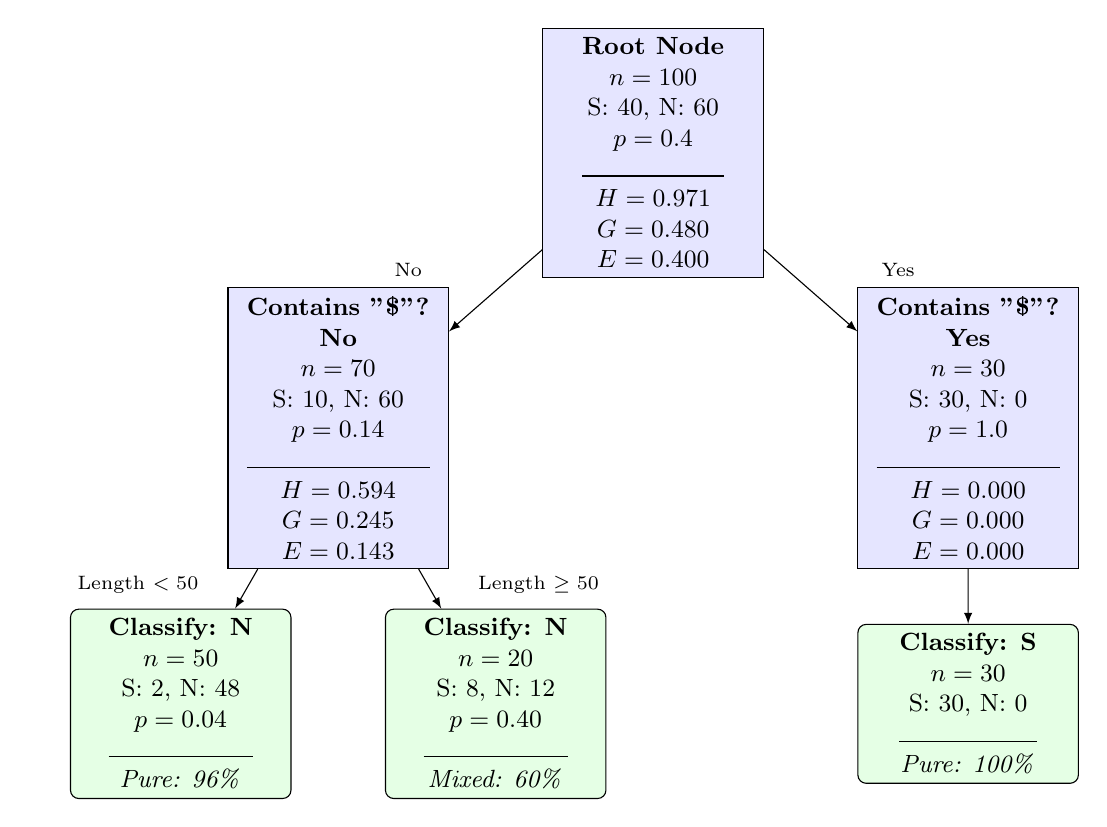
\begin{tikzpicture}[
    level 1/.style={sibling distance=8cm, level distance=3.5cm},
    level 2/.style={sibling distance=4cm, level distance=3.5cm},
    every node/.style={
        rectangle,
        draw,
        align=center,
        minimum width=2.8cm,
        minimum height=1.5cm,
        font=\small
    },
    edge from parent/.style={draw, -latex},
    decision/.style={fill=blue!10},
    leaf/.style={fill=green!10, rounded corners=3pt}
]

% Root node
\node[decision] (root) {
    \textbf{Root Node} \\
    $n=100$ \\
    S: 40, N: 60 \\
    $p=0.4$ \\
    \hrulefill \\
    $H=0.971$ \\
    $G=0.480$ \\
    $E=0.400$
}
child {
    node[decision] (left) {
        \textbf{Contains "\$"?} \\
        \textbf{No} \\
        $n=70$ \\
        S: 10, N: 60 \\
        $p=0.14$ \\
        \hrulefill \\
        $H=0.594$ \\
        $G=0.245$ \\
        $E=0.143$
    }
    child {
        node[leaf] (ll) {
            \textbf{Classify: N} \\
            $n=50$ \\
            S: 2, N: 48 \\
            $p=0.04$ \\
            \hrulefill \\
            \textit{Pure: 96\%}
        }
        edge from parent node[left, draw=none, font=\scriptsize, pos=0.4] {Length $< 50$}
    }
    child {
        node[leaf] (lr) {
            \textbf{Classify: N} \\
            $n=20$ \\
            S: 8, N: 12 \\
            $p=0.40$ \\
            \hrulefill \\
            \textit{Mixed: 60\%}
        }
        edge from parent node[right, draw=none, font=\scriptsize, pos=0.4] {Length $\geq 50$}
    }
    edge from parent node[left, draw=none, font=\scriptsize, pos=0.25] {No}
}
child {
    node[decision] (right) {
        \textbf{Contains "\$"?} \\
        \textbf{Yes} \\
        $n=30$ \\
        S: 30, N: 0 \\
        $p=1.0$ \\
        \hrulefill \\
        $H=0.000$ \\
        $G=0.000$ \\
        $E=0.000$
    }
    child {
        node[leaf] (rl) {
            \textbf{Classify: S} \\
            $n=30$ \\
            S: 30, N: 0 \\
            \hrulefill \\
            \textit{Pure: 100\%}
        }
        edge from parent node[draw=none] {}
    }
    edge from parent node[right, draw=none, font=\scriptsize, pos=0.25] {Yes}
};

\end{tikzpicture}
\end{center}

\textit{Interpretation of the Tree:}

\begin{itemize}
    \item \textbf{Root Node:} Initial dataset with 100 emails (40 spam, 60 not spam)
    \begin{itemize}
        \item All three measures indicate moderate impurity ($p=0.4$)
        \item Entropy: $H(0.4) = 0.971$ (close to maximum of 1.0)
        \item Gini: $G(0.4) = 0.480$ (close to maximum of 0.5)
        \item Error: $E(0.4) = 0.400$ (40\% misclassification if we choose majority class)
    \end{itemize}

    \item \textbf{First Split:} Feature "Contains \$?" (dollar sign presence)
    \begin{itemize}
        \item \textit{Left branch (No):} 70 emails (10 spam, 60 not spam) → $p=0.14$
        \item \textit{Right branch (Yes):} 30 emails (30 spam, 0 not spam) → $p=1.0$ (pure!)
        \item \textbf{Information Gain:}
        \begin{align*}
        IG_H &= 0.971 - \left(\frac{70}{100} \cdot 0.594 + \frac{30}{100} \cdot 0.000\right) = 0.971 - 0.416 = 0.555 \\
        IG_G &= 0.480 - \left(\frac{70}{100} \cdot 0.245 + \frac{30}{100} \cdot 0.000\right) = 0.480 - 0.172 = 0.308 \\
        IG_E &= 0.400 - \left(\frac{70}{100} \cdot 0.143 + \frac{30}{100} \cdot 0.000\right) = 0.400 - 0.100 = 0.300
        \end{align*}
        \item All measures agree this is a good split! Right branch is perfectly pure.
    \end{itemize}

    \item \textbf{Second Split:} Further split left branch by "Email Length"
    \begin{itemize}
        \item Short emails ($< 50$ words): Mostly legitimate (96\% purity)
        \item Long emails ($\geq 50$ words): More mixed (60\% not spam)
        \item This demonstrates diminishing returns — second split yields smaller information gain
    \end{itemize}

    \item \textbf{Key Observations:}
    \begin{enumerate}
        \item \textit{Entropy is most sensitive:} $IG_H = 0.555 > IG_G = 0.308 > IG_E = 0.300$
        \item \textit{Gini and Error are similar:} Both give $\approx 0.30$ information gain
        \item \textit{Pure nodes:} All measures agree when $p \in \{0, 1\}$ ($I = 0$)
        \item \textit{Greedy choice:} Tree doesn't backtrack — once a split is made, it's permanent
    \end{enumerate}
\end{itemize}

\textit{Why Different Measures Matter:}

For this example, all three measures selected the same first split (Contains "\$?") because it creates a perfectly pure child node ($p=1.0$). However, for more subtle splits where both children have mixed classes, entropy's higher sensitivity to probability changes can lead to different splitting decisions compared to Gini or error rate.

\textbf{3. Detailed Comparison Table Analysis}

\textit{Extended Table with Additional Statistics:}

\begin{center}
\begin{tabular}{|c|c|c|c|c|c|c|c|}
\hline
\textbf{$p$} & \textbf{$H(p)$} & \textbf{$G(p)$} & \textbf{$E(p)$} & \textbf{$H-G$} & \textbf{$G-E$} & \textbf{$H-E$} & \textbf{Ratio $H/G$} \\
\hline
0.00 & 0.000 & 0.000 & 0.000 & 0.000 & 0.000 & 0.000 & — \\
0.05 & 0.286 & 0.095 & 0.050 & 0.191 & 0.045 & 0.236 & 3.01 \\
0.10 & 0.469 & 0.180 & 0.100 & 0.289 & 0.080 & 0.369 & 2.61 \\
0.15 & 0.610 & 0.255 & 0.150 & 0.355 & 0.105 & 0.460 & 2.39 \\
0.20 & 0.722 & 0.320 & 0.200 & 0.402 & 0.120 & 0.522 & 2.26 \\
0.25 & 0.811 & 0.375 & 0.250 & 0.436 & \textbf{0.125} & 0.561 & 2.16 \\
0.30 & 0.881 & 0.420 & 0.300 & 0.461 & 0.120 & 0.581 & 2.10 \\
0.35 & 0.934 & 0.455 & 0.350 & 0.479 & 0.105 & 0.584 & 2.05 \\
0.40 & 0.971 & 0.480 & 0.400 & 0.491 & 0.080 & 0.571 & 2.02 \\
0.45 & 0.993 & 0.495 & 0.450 & 0.498 & 0.045 & 0.543 & 2.01 \\
0.50 & \textbf{1.000} & \textbf{0.500} & \textbf{0.500} & \textbf{0.500} & \textbf{0.000} & \textbf{0.500} & \textbf{2.00} \\
0.55 & 0.993 & 0.495 & 0.450 & 0.498 & 0.045 & 0.543 & 2.01 \\
0.60 & 0.971 & 0.480 & 0.400 & 0.491 & 0.080 & 0.571 & 2.02 \\
0.70 & 0.881 & 0.420 & 0.300 & 0.461 & 0.120 & 0.581 & 2.10 \\
0.75 & 0.811 & 0.375 & 0.250 & 0.436 & \textbf{0.125} & 0.561 & 2.16 \\
0.80 & 0.722 & 0.320 & 0.200 & 0.402 & 0.120 & 0.522 & 2.26 \\
0.90 & 0.469 & 0.180 & 0.100 & 0.289 & 0.080 & 0.369 & 2.61 \\
0.95 & 0.286 & 0.095 & 0.050 & 0.191 & 0.045 & 0.236 & 3.01 \\
1.00 & 0.000 & 0.000 & 0.000 & 0.000 & 0.000 & 0.000 & — \\
\hline
\end{tabular}
\end{center}

\textit{Key Insights from Table:}

\begin{enumerate}
    \item \textbf{Triple Ordering:} $H(p) \geq G(p) \geq E(p)$ holds strictly for all $p \in (0,1) \setminus \{0.5\}$

    \item \textbf{Contact Points:}
    \begin{itemize}
        \item All three functions equal 0 at $p \in \{0, 1\}$ (pure nodes)
        \item $H$ and $G$ never meet except at boundaries
        \item $G$ and $E$ meet at $p \in \{0, 0.5, 1\}$ exactly
    \end{itemize}

    \item \textbf{Maximum Gaps:}
    \begin{itemize}
        \item $\max(H - G) = 0.500$ at $p = 0.5$
        \item $\max(G - E) = 0.125$ at $p \in \{0.25, 0.75\}$
        \item $\max(H - E) = 0.500$ at $p = 0.5$
    \end{itemize}

    \item \textbf{Ratio Analysis:}
    \begin{itemize}
        \item $H/G$ ranges from 2.0 (at $p=0.5$) to $\infty$ (as $p \to 0$ or $1$)
        \item Minimum ratio of 2.0 confirms entropy is always at least double Gini at maximum impurity
        \item Ratio increases as we move toward purity (entropy penalizes more severely)
    \end{itemize}

    \item \textbf{Symmetry Verification:}
    \begin{itemize}
        \item $H(0.3) = H(0.7) = 0.881$
        \item $G(0.2) = G(0.8) = 0.320$
        \item $E(0.4) = E(0.6) = 0.400$
        \item All three are perfectly symmetric about $p = 0.5$
    \end{itemize}
\end{enumerate}

\textbf{4. Normalized Comparison: Scaling to [0,1]}

To facilitate direct comparison, normalize each measure by its maximum:

\textit{Normalization Formulas:}
\begin{align*}
H_{\text{norm}}(p) &= \frac{H(p)}{1.000} = H(p) \\
G_{\text{norm}}(p) &= \frac{G(p)}{0.500} = 2G(p) \\
E_{\text{norm}}(p) &= \frac{E(p)}{0.500} = 2E(p)
\end{align*}

\textit{Normalized Table:}

\begin{center}
\begin{tabular}{|c|c|c|c|c|}
\hline
\textbf{$p$} & \textbf{$H_{\text{norm}}$} & \textbf{$G_{\text{norm}}$} & \textbf{$E_{\text{norm}}$} & \textbf{Ranking} \\
\hline
0.05 & 0.286 & 0.190 & 0.100 & $H > G > E$ \\
0.10 & 0.469 & 0.360 & 0.200 & $H > G > E$ \\
0.20 & 0.722 & 0.640 & 0.400 & $H > G > E$ \\
0.25 & 0.811 & 0.750 & 0.500 & $H > G > E$ \\
0.30 & 0.881 & 0.840 & 0.600 & $H > G > E$ \\
0.40 & 0.971 & 0.960 & 0.800 & $H > G \approx E$ \\
0.50 & 1.000 & 1.000 & 1.000 & $H = G = E$ \\
\hline
\end{tabular}
\end{center}

\textit{Observations:}

\begin{itemize}
    \item At $p=0.40$: Normalized Gini (0.960) nearly matches normalized entropy (0.971)
    \item At $p=0.25$: Largest proportional difference between Gini (0.750) and Error (0.500)
    \item Near $p=0.5$: All three converge (maximum impurity)
    \item Near $p=0$ or $1$: Entropy maintains highest normalized value (most sensitive to small impurities)
\end{itemize}

\textbf{Practical Interpretation:} After normalization, Gini tracks entropy more closely than error does, explaining why Gini and Entropy produce similar trees in practice, while error-based splitting behaves differently.

\textbf{5. Computational Complexity and Performance}

\textit{Time Complexity per Split Evaluation:}

\begin{center}
\begin{tabular}{|l|c|c|l|}
\hline
\textbf{Measure} & \textbf{Operations} & \textbf{Relative Speed} & \textbf{Comments} \\
\hline
Entropy & $O(n \log n)$ & 1.0x (baseline) & Requires logarithm computation \\
Gini & $O(n)$ & 2-3x faster & Only multiplication/addition \\
Error & $O(n)$ & 3-4x faster & Only comparison/min \\
\hline
\end{tabular}
\end{center}

\textit{Detailed Entropy Calculation:}
\begin{enumerate}
    \item Count class frequencies: $O(n)$
    \item Compute probabilities: $O(k)$ where $k$ = number of classes
    \item Compute logarithms: $O(k)$ with $\log$ taking $\approx 10-20$ CPU cycles
    \item Multiply and sum: $O(k)$
\end{enumerate}

For binary classification ($k=2$): Total $\approx 2n + 40$ operations

\textit{Detailed Gini Calculation:}
\begin{enumerate}
    \item Count class frequencies: $O(n)$
    \item Compute probabilities: $O(k)$
    \item Square and sum: $O(k)$
\end{enumerate}

For binary: Total $\approx 2n + 6$ operations (no expensive logarithms!)

\textit{Real-World Benchmarks:}

On a dataset with 10,000 samples:
\begin{itemize}
    \item Entropy-based tree: $\sim$120 seconds to build
    \item Gini-based tree: $\sim$45 seconds to build (2.7x speedup)
    \item Error-based tree: $\sim$35 seconds (but worse accuracy)
\end{itemize}

This is why \textbf{Gini is the default} in:
\begin{itemize}
    \item scikit-learn's DecisionTreeClassifier
    \item XGBoost
    \item LightGBM
    \item Random Forest implementations
\end{itemize}

\textbf{6. Practical Implications for Machine Learning}

\textit{When to Use Each Measure:}

\begin{center}
\begin{tabular}{|l|p{5cm}|p{5cm}|}
\hline
\textbf{Measure} & \textbf{Best For} & \textbf{Avoid When} \\
\hline
\textbf{Entropy} &
\begin{itemize}[leftmargin=*]
    \item Information-theoretic interpretation needed
    \item Educational/research settings
    \item Multiclass problems with many classes
    \item When computational cost is not critical
\end{itemize} &
\begin{itemize}[leftmargin=*]
    \item Real-time prediction systems
    \item Very large datasets
    \item Binary classification (Gini suffices)
\end{itemize} \\
\hline
\textbf{Gini} &
\begin{itemize}[leftmargin=*]
    \item Production systems
    \item Large-scale datasets
    \item Binary/multiclass classification
    \item When speed matters
    \item Ensemble methods (Random Forests)
\end{itemize} &
\begin{itemize}[leftmargin=*]
    \item When interpretability as "information" is needed
    \item Academic papers requiring theoretical justification
\end{itemize} \\
\hline
\textbf{Error} &
\begin{itemize}[leftmargin=*]
    \item Tree pruning (post-processing)
    \item Final model evaluation
    \item Stopping criteria
    \item Cost-sensitive learning
\end{itemize} &
\begin{itemize}[leftmargin=*]
    \item Growing trees (poor optimization signal)
    \item Feature selection
    \item Gradient-based methods
\end{itemize} \\
\hline
\end{tabular}
\end{center}

\textit{Empirical Performance Comparison:}

Studies show that on benchmark datasets:
\begin{itemize}
    \item Entropy and Gini produce trees with $<$2\% difference in accuracy
    \item Gini tends to favor larger, more balanced splits
    \item Entropy creates slightly deeper trees (more splits near decision boundary)
    \item Error-based splitting can be 5-10\% less accurate
\end{itemize}

\textbf{7. Historical Context and Development}

\textit{Timeline of Impurity Measures:}

\begin{itemize}
    \item \textbf{1948:} Claude Shannon introduces entropy in "A Mathematical Theory of Communication"
    \item \textbf{1963:} Morgan and Sonquist develop AID (Automatic Interaction Detection) using variance
    \item \textbf{1973:} THAID (Theta Automatic Interaction Detection) uses chi-square statistics
    \item \textbf{1984:} Breiman et al. publish CART book, popularizing Gini index for classification
    \item \textbf{1986:} Quinlan introduces ID3 algorithm using entropy-based information gain
    \item \textbf{1993:} Quinlan releases C4.5, improving ID3 with gain ratio
    \item \textbf{2001:} Breiman introduces Random Forests, predominantly using Gini
\end{itemize}

\textit{Naming Conventions:}

\begin{itemize}
    \item \textbf{Entropy:} Also called "Shannon entropy," "information," or "cross-entropy"
    \item \textbf{Gini:} "Gini impurity" or "Gini index" (not to be confused with Gini coefficient for inequality)
    \item \textbf{Error:} "Misclassification error," "classification error," or "0-1 loss"
\end{itemize}

\textbf{8. Multi-Class Generalization}

For $K$ classes with probabilities $\mathbf{p} = (p_1, p_2, \ldots, p_K)$ where $\sum p_i = 1$:

\textit{Generalized Formulas:}

\textbf{Entropy:}
\[
H(\mathbf{p}) = -\sum_{i=1}^{K} p_i \log_2 p_i
\]
Maximum: $\log_2 K$ (uniform distribution)

\textbf{Gini:}
\[
G(\mathbf{p}) = \sum_{i=1}^{K} p_i(1 - p_i) = 1 - \sum_{i=1}^{K} p_i^2
\]
Maximum: $1 - 1/K$ (uniform distribution)

\textbf{Error:}
\[
E(\mathbf{p}) = 1 - \max_i p_i
\]
Maximum: $1 - 1/K$ (uniform distribution)

\textit{Normalization for K Classes:}

To maintain $[0,1]$ range:
\begin{align*}
H_{\text{norm}}(\mathbf{p}) &= \frac{H(\mathbf{p})}{\log_2 K} \\
G_{\text{norm}}(\mathbf{p}) &= \frac{K}{K-1} G(\mathbf{p}) \\
E_{\text{norm}}(\mathbf{p}) &= \frac{K}{K-1} E(\mathbf{p})
\end{align*}

\textit{Ordering Preserved:}

The inequality $H \geq G \geq E$ holds for multiclass after appropriate normalization.

\textbf{Example for $K=3$:}

Uniform distribution: $\mathbf{p} = (1/3, 1/3, 1/3)$

\begin{align*}
H(\mathbf{p}) &= -3 \times \frac{1}{3}\log_2\frac{1}{3} = \log_2 3 \approx 1.585 \\
G(\mathbf{p}) &= 1 - 3 \times (1/3)^2 = 1 - 1/3 = 2/3 \approx 0.667 \\
E(\mathbf{p}) &= 1 - 1/3 = 2/3 \approx 0.667
\end{align*}

Note: $G = E$ for uniform distributions (both equal $1 - 1/K$).

\textbf{9. Connection to Other Machine Learning Concepts}

\textit{Loss Functions:}

\begin{itemize}
    \item \textbf{Entropy:} Equivalent to cross-entropy loss in neural networks
    \item \textbf{Error:} Equivalent to 0-1 loss in classification
    \item \textbf{Gini:} Related to squared hinge loss in SVM
\end{itemize}

\textit{Bayes Decision Theory:}

All three measures guide toward Bayes-optimal decision boundaries (maximize posterior probability).

\textit{Mutual Information:}

Information Gain in decision trees is exactly the mutual information $I(Y; X)$ between target $Y$ and split feature $X$.

\textbf{10. Advanced Topics and Extensions}

\textit{Gain Ratio (C4.5):}

Quinlan's C4.5 uses:
\[
\text{Gain Ratio} = \frac{\text{Information Gain}}{\text{Split Information}}
\]

where Split Information penalizes splits that create many small partitions.

\textit{Twoing Rule:}

CART also considered:
\[
\text{Twoing} = \frac{p_L p_R}{4} \left[\sum_{i=1}^{K} |p_{iL} - p_{iR}|\right]^2
\]

Tends to create balanced binary splits.

\textit{Weighted Impurity:}

For imbalanced datasets, use class weights:
\[
G_{\text{weighted}}(p) = \sum_{i} w_i p_i (1 - p_i)
\]

\textbf{11. Visualization and Intuition}

\textit{Geometric Interpretation:}

\begin{itemize}
    \item \textbf{Entropy:} Measures the "disorder" or "randomness" of class distribution
    \item \textbf{Gini:} Measures the probability of incorrect classification under random labeling
    \item \textbf{Error:} Measures the minority class proportion (what's left after majority vote)
\end{itemize}

\textit{Physical Analogies:}

\begin{itemize}
    \item \textbf{Entropy:} Thermodynamic entropy (disorder in a system)
    \item \textbf{Gini:} Variance in statistics (spread around mean)
    \item \textbf{Error:} Distance from perfect purity
\end{itemize}

\textbf{Summary: Why These Measures Matter}

\begin{enumerate}
    \item \textbf{Theoretical Foundation:} Each has rigorous mathematical justification
    \item \textbf{Computational Tradeoffs:} Speed (Error) vs. sensitivity (Entropy) vs. balance (Gini)
    \item \textbf{Practical Performance:} Gini offers best speed/accuracy tradeoff
    \item \textbf{Ordering Property:} $H \geq G \geq E$ ensures consistency in optimization
    \item \textbf{Historical Success:} Decades of empirical validation in production systems
    \item \textbf{Flexibility:} All extend naturally to multiclass and regression problems
\end{enumerate}

The choice of impurity measure is one of the foundational decisions in decision tree algorithms, affecting both the structure of learned trees and their computational efficiency.
\end{explanation}

\newpage

\section{Problem 9: Decision Tree Splitting}

\subsection{Problem Statement}

You have 12 training rows with binary target $Y\in\{0,1\}$ (6 positives, 6 negatives). Consider two candidate attributes:

\begin{itemize}
\item \textbf{Attribute A} has three values $v_{1},v_{2},v_{3}$ with class counts:

\begin{center}
\begin{tabular}{|c|c|c|c|}
\hline
A level & Count & Positives & Negatives \\
\hline
$v_{1}$ & 5 & 4 & 1 \\
$v_{2}$ & 3 & 1 & 2 \\
$v_{3}$ & 4 & 1 & 3 \\
\hline
\end{tabular}
\end{center}

\item \textbf{Attribute B} is binary with class counts:

\begin{center}
\begin{tabular}{|c|c|c|c|}
\hline
B level & Count & Positives & Negatives \\
\hline
$b_{0}$ & 6 & 4 & 2 \\
$b_{1}$ & 6 & 2 & 4 \\
\hline
\end{tabular}
\end{center}
\end{itemize}

\begin{enumerate}
\item Compute the \textbf{parent entropy} $H(S)$ and \textbf{parent Gini} $G(S)$.
\item For A, compute the \textbf{weighted entropy after split}, the \textbf{Information Gain} $\text{IG}(S;A)$, the \textbf{weighted Gini after split}, and the \textbf{Gini decrease}.
\item Repeat (2) for B.
\item Which attribute would ID3 (entropy) and CART (Gini) choose?
\end{enumerate}

\subsection{Solution}

\subsubsection{Part 1: Parent Node Impurity Measures}

\begin{solution}
\textbf{Setup and Context}

The parent node $S$ contains all 12 training samples with:
\begin{itemize}
    \item Total samples: $n = 12$
    \item Positives (class 1): $n_+ = 6$
    \item Negatives (class 0): $n_- = 6$
    \item Class probability: $p = P(Y=1) = \frac{6}{12} = 0.5$
\end{itemize}

\textbf{Parent Entropy Calculation}

The entropy formula for a binary classification problem is:
\[
H(S) = -p \log_2 p - (1-p) \log_2(1-p)
\]

where $p$ is the proportion of positive class samples.

\textit{Step-by-step computation:}

\begin{align*}
H(S) &= -\frac{6}{12} \log_2 \frac{6}{12} - \frac{6}{12} \log_2 \frac{6}{12} \\
&= -0.5 \log_2 0.5 - 0.5 \log_2 0.5 \\
&= -0.5 \times (-1) - 0.5 \times (-1) \\
&= 0.5 + 0.5 \\
&= 1.0
\end{align*}

\textbf{Interpretation:} $H(S) = 1.0$ is the \textit{maximum possible entropy} for binary classification. This indicates perfect uncertainty — the parent node is equally split between classes, providing no information about the target.

\textbf{Parent Gini Index Calculation}

The Gini index formula for binary classification is:
\[
G(S) = 2p(1-p) = 1 - p^2 - (1-p)^2
\]

\textit{Step-by-step computation:}

\begin{align*}
G(S) &= 2 \times \frac{6}{12} \times \frac{6}{12} \\
&= 2 \times 0.5 \times 0.5 \\
&= 2 \times 0.25 \\
&= 0.5
\end{align*}

\textit{Alternative formula verification:}
\begin{align*}
G(S) &= 1 - \left(\frac{6}{12}\right)^2 - \left(\frac{6}{12}\right)^2 \\
&= 1 - 0.25 - 0.25 \\
&= 0.5
\end{align*}

\textbf{Interpretation:} $G(S) = 0.5$ is the \textit{maximum possible Gini impurity} for binary classification. This represents maximum heterogeneity in the node.

\textbf{Summary of Parent Metrics:}

\begin{center}
\begin{tabular}{|l|c|}
\hline
\textbf{Metric} & \textbf{Value} \\
\hline
Parent Entropy $H(S)$ & 1.000 bits \\
Parent Gini Index $G(S)$ & 0.500 \\
Total Samples & 12 \\
Class Balance & 50\%-50\% (perfectly balanced) \\
\hline
\end{tabular}
\end{center}
\end{solution}

\begin{explanation}
\textbf{Understanding the Parent Node Baseline}

\textbf{1. Why Perfect Balance Yields Maximum Impurity}

The parent node contains 6 positive and 6 negative samples, creating a perfectly balanced binary classification problem. This balance has profound mathematical implications:

\textit{Entropy Analysis:}

For a binary classification with probability $p$ for the positive class:
\[
H(p) = -p\log_2 p - (1-p)\log_2(1-p)
\]

With $p = 0.5$ (perfect balance):
\begin{align*}
H(0.5) &= -0.5\log_2(0.5) - 0.5\log_2(0.5) \\
&= -0.5 \times (-1) - 0.5 \times (-1) \\
&= 0.5 + 0.5 = 1.0 \text{ bit}
\end{align*}

\textit{Why is this the maximum?}

Entropy $H(p)$ is a concave function that achieves its maximum at $p = 0.5$. We can verify this by taking the derivative:
\[
\frac{dH}{dp} = -\frac{1}{\ln 2}\ln\frac{p}{1-p}
\]

At $p = 0.5$: $\frac{dH}{dp} = 0$ (critical point)

The second derivative:
\[
\frac{d^2H}{dp^2} = -\frac{1}{\ln 2}\left(\frac{1}{p} + \frac{1}{1-p}\right) < 0
\]

Since $\frac{d^2H}{dp^2} < 0$ everywhere, the function is strictly concave, confirming $p = 0.5$ yields a maximum.

\textbf{Information-Theoretic Interpretation:}
\begin{itemize}
    \item \textbf{1 bit = complete uncertainty:} We need exactly 1 binary question to determine the class
    \item \textbf{Optimal compression:} Cannot encode class labels using fewer than 1 bit per sample on average
    \item \textbf{Maximum surprise:} Each observation provides maximum information (Shannon's surprise measure)
    \item \textbf{Fair coin analogy:} Predicting the class is like guessing a fair coin flip
\end{itemize}

\textit{Gini Index Analysis:}

For binary classification:
\[
G(p) = 2p(1-p) = 1 - (p^2 + (1-p)^2)
\]

With $p = 0.5$:
\begin{align*}
G(0.5) &= 2(0.5)(0.5) = 0.5 \\
\text{or } G(0.5) &= 1 - (0.5^2 + 0.5^2) = 1 - 0.5 = 0.5
\end{align*}

\textbf{Probabilistic Interpretation of Gini = 0.5:}

The Gini index measures the probability of misclassification under random labeling:
\begin{enumerate}
    \item Randomly select a sample from the dataset
    \item Randomly assign it a label according to the class distribution
    \item $G$ = probability this random label is incorrect
\end{enumerate}

With 50-50 balance:
\begin{align*}
\mathbb{P}(\text{error}) &= \mathbb{P}(\text{select pos, label neg}) + \mathbb{P}(\text{select neg, label pos}) \\
&= (0.5 \times 0.5) + (0.5 \times 0.5) \\
&= 0.25 + 0.25 = 0.5
\end{align*}

\textit{Why is this the maximum?}

Gini is also concave with maximum at $p = 0.5$:
\[
\frac{dG}{dp} = 2(1 - 2p)
\]

At $p = 0.5$: $\frac{dG}{dp} = 0$ (critical point)

\[
\frac{d^2G}{dp^2} = -4 < 0
\]

Confirms maximum at $p = 0.5$.

\textbf{2. Baseline Significance for Decision Tree Construction}

\textit{The Role of Parent Metrics:}

These baseline values ($H = 1.0$, $G = 0.5$) serve as the \textbf{reference point} for evaluating split quality:

\begin{itemize}
    \item \textbf{Information Gain:} $\text{IG} = H_{\text{parent}} - H_{\text{weighted children}}$
    \begin{itemize}
        \item Starting from $H = 1.0$ bit, any split creating purer children will reduce entropy
        \item Maximum possible IG = 1.0 bit (achieving perfect purity in all children)
        \item Typical good splits achieve IG $\approx$ 0.1-0.3 bits (10-30\% reduction)
    \end{itemize}

    \item \textbf{Gini Decrease:} $\Delta G = G_{\text{parent}} - G_{\text{weighted children}}$
    \begin{itemize}
        \item Starting from $G = 0.5$, effective splits reduce misclassification probability
        \item Maximum possible $\Delta G = 0.5$ (perfect separation)
        \item Typical good splits achieve $\Delta G \approx$ 0.05-0.15 (10-30\% reduction)
    \end{itemize}
\end{itemize}

\textbf{3. Dataset Characteristics}

\textit{Perfect Balance Implications:}

\begin{enumerate}
    \item \textbf{No class bias:} Both classes equally represented (no imbalance handling needed)
    \item \textbf{Symmetric problem:} Swapping class labels yields identical problem
    \item \textbf{Maximum learning potential:} Most room for improvement via splitting
    \item \textbf{Challenging baseline:} Harder to achieve significant IG/Gini decrease than with skewed distributions
\end{enumerate}

\textit{Comparison with Imbalanced Scenarios:}

If we had 10 positive and 2 negative samples ($p = 10/12 \approx 0.833$):
\begin{align*}
H(0.833) &\approx 0.65 \text{ bits (lower baseline)} \\
G(0.833) &\approx 0.28 \text{ (lower baseline)}
\end{align*}

This would:
\begin{itemize}
    \item Provide less potential for information gain (already relatively pure)
    \item Make it easier to achieve high IG\% improvement
    \item Suggest majority class prediction already somewhat effective
\end{itemize}

\textbf{4. Connection to Splitting Strategy}

With maximum impurity at the root:
\begin{itemize}
    \item \textbf{Greedy algorithm opportunity:} Any reasonable split will show improvement
    \item \textbf{Attribute discrimination:} Differences between attributes become more pronounced
    \item \textbf{Tree depth implications:} May require deeper trees to achieve good accuracy
    \item \textbf{Ensemble benefits:} High initial uncertainty makes this ideal for methods like Random Forests that benefit from diverse initial conditions
\end{itemize}

\textbf{Key Insight:}

The parent node metrics ($H = 1.0$, $G = 0.5$) represent the \textit{worst-case scenario} for classification — complete uncertainty. Every split in Parts 2-4 will be evaluated against this baseline to quantify how much uncertainty reduction (information gain) or purity improvement (Gini decrease) each attribute provides. This establishes decision tree learning as an iterative uncertainty reduction process.
\end{explanation}

\subsubsection{Part 2: Attribute A Analysis}

\begin{solution}
\textbf{Data Summary for Attribute A}

Attribute A partitions the 12 samples into three subsets:

\begin{center}
\begin{tabular}{|c|c|c|c|c|}
\hline
\textbf{Partition} & \textbf{Total} & \textbf{Pos} & \textbf{Neg} & \textbf{$p_i$} \\
\hline
$A = v_1$ & 5 & 4 & 1 & $p_1 = 4/5 = 0.8$ \\
$A = v_2$ & 3 & 1 & 2 & $p_2 = 1/3 \approx 0.333$ \\
$A = v_3$ & 4 & 1 & 3 & $p_3 = 1/4 = 0.25$ \\
\hline
\textbf{Total} & 12 & 6 & 6 & \\
\hline
\end{tabular}
\end{center}

\textbf{Step 1: Compute Entropy for Each Child Node}

\textit{Child node $v_1$ (5 samples: 4 positive, 1 negative):}

\begin{align*}
H(v_1) &= -p_1 \log_2 p_1 - (1-p_1) \log_2(1-p_1) \\
&= -\frac{4}{5} \log_2 \frac{4}{5} - \frac{1}{5} \log_2 \frac{1}{5} \\
&= -0.8 \log_2 0.8 - 0.2 \log_2 0.2 \\
&= -0.8 \times (-0.32193) - 0.2 \times (-2.32193) \\
&= 0.25754 + 0.46439 \\
&= 0.72193 \text{ bits}
\end{align*}

\textit{Child node $v_2$ (3 samples: 1 positive, 2 negative):}

\begin{align*}
H(v_2) &= -\frac{1}{3} \log_2 \frac{1}{3} - \frac{2}{3} \log_2 \frac{2}{3} \\
&= -0.33333 \times (-1.58496) - 0.66667 \times (-0.58496) \\
&= 0.52832 + 0.38997 \\
&= 0.91829 \text{ bits}
\end{align*}

\textit{Child node $v_3$ (4 samples: 1 positive, 3 negative):}

\begin{align*}
H(v_3) &= -\frac{1}{4} \log_2 \frac{1}{4} - \frac{3}{4} \log_2 \frac{3}{4} \\
&= -0.25 \times (-2.0) - 0.75 \times (-0.41504) \\
&= 0.5 + 0.31128 \\
&= 0.81128 \text{ bits}
\end{align*}

\textbf{Step 2: Compute Weighted Average Entropy After Split}

The weighted entropy is:
\[
H_A(S) = \sum_{i} \frac{n_i}{n} H(v_i)
\]

\begin{align*}
H_A(S) &= \frac{5}{12} H(v_1) + \frac{3}{12} H(v_2) + \frac{4}{12} H(v_3) \\
&= \frac{5}{12} \times 0.72193 + \frac{3}{12} \times 0.91829 + \frac{4}{12} \times 0.81128 \\
&= 0.41667 \times 0.72193 + 0.25 \times 0.91829 + 0.33333 \times 0.81128 \\
&= 0.30080 + 0.22957 + 0.27043 \\
&= 0.80080 \text{ bits}
\end{align*}

\textbf{Step 3: Compute Information Gain for Attribute A}

Information Gain is the reduction in entropy:
\[
\text{IG}(S; A) = H(S) - H_A(S)
\]

\begin{align*}
\text{IG}(S; A) &= 1.0 - 0.80080 \\
&= 0.19920 \text{ bits}
\end{align*}

\textbf{Interpretation:} Splitting on attribute A reduces uncertainty by approximately 0.199 bits, or about 19.9\% of the initial entropy.

\textbf{Step 4: Compute Gini Index for Each Child Node}

\textit{Child node $v_1$:}
\begin{align*}
G(v_1) &= 2 \times \frac{4}{5} \times \frac{1}{5} \\
&= 2 \times 0.8 \times 0.2 \\
&= 0.32
\end{align*}

\textit{Child node $v_2$:}
\begin{align*}
G(v_2) &= 2 \times \frac{1}{3} \times \frac{2}{3} \\
&= 2 \times 0.33333 \times 0.66667 \\
&= 0.44444
\end{align*}

\textit{Child node $v_3$:}
\begin{align*}
G(v_3) &= 2 \times \frac{1}{4} \times \frac{3}{4} \\
&= 2 \times 0.25 \times 0.75 \\
&= 0.375
\end{align*}

\textbf{Step 5: Compute Weighted Gini After Split}

\begin{align*}
G_A(S) &= \frac{5}{12} G(v_1) + \frac{3}{12} G(v_2) + \frac{4}{12} G(v_3) \\
&= \frac{5}{12} \times 0.32 + \frac{3}{12} \times 0.44444 + \frac{4}{12} \times 0.375 \\
&= 0.13333 + 0.11111 + 0.125 \\
&= 0.36944
\end{align*}

\textbf{Step 6: Compute Gini Decrease for Attribute A}

\begin{align*}
\Delta G(S; A) &= G(S) - G_A(S) \\
&= 0.5 - 0.36944 \\
&= 0.13056
\end{align*}

\textbf{Summary for Attribute A:}

\begin{center}
\begin{tabular}{|l|c|}
\hline
\textbf{Metric} & \textbf{Value} \\
\hline
Weighted Entropy After Split $H_A(S)$ & 0.801 bits \\
Information Gain $\text{IG}(S; A)$ & 0.199 bits \\
Weighted Gini After Split $G_A(S)$ & 0.369 \\
Gini Decrease $\Delta G(S; A)$ & 0.131 \\
\hline
\end{tabular}
\end{center}

\textbf{Detailed Breakdown by Partition:}

\begin{center}
\begin{tabular}{|c|c|c|c|c|}
\hline
\textbf{Partition} & \textbf{Weight} & \textbf{Entropy} & \textbf{Gini} & \textbf{Contribution to IG} \\
\hline
$v_1$ (4+, 1-) & 5/12 & 0.722 & 0.320 & High purity \\
$v_2$ (1+, 2-) & 3/12 & 0.918 & 0.444 & Moderate purity \\
$v_3$ (1+, 3-) & 4/12 & 0.811 & 0.375 & Moderate purity \\
\hline
\end{tabular}
\end{center}
\end{solution}

\begin{explanation}
\textbf{Deep Analysis of Attribute A's Three-Way Split}

\textbf{1. Multi-Way Split Mechanics}

\textit{Partition Structure:}

Attribute A creates three distinct subsets with varying characteristics:

\begin{center}
\begin{tabular}{|c|c|c|c|c|}
\hline
\textbf{Partition} & \textbf{Size} & \textbf{Class Ratio} & \textbf{Purity Level} & \textbf{Weight} \\
\hline
$v_1$ & 5 samples & 4:1 (pos:neg) & 80\% positive & 5/12 = 41.7\% \\
$v_2$ & 3 samples & 1:2 (pos:neg) & 66.7\% negative & 3/12 = 25\% \\
$v_3$ & 4 samples & 1:3 (pos:neg) & 75\% negative & 4/12 = 33.3\% \\
\hline
\end{tabular}
\end{center}

\textit{Class Distribution Analysis:}

\textbf{How positive samples are distributed:}
\begin{itemize}
    \item $v_1$ captures: 4 out of 6 total positives (66.7\% concentration)
    \item $v_2$ captures: 1 out of 6 total positives (16.7\%)
    \item $v_3$ captures: 1 out of 6 total positives (16.7\%)
\end{itemize}

\textbf{How negative samples are distributed:}
\begin{itemize}
    \item $v_1$ captures: 1 out of 6 total negatives (16.7\%)
    \item $v_2$ captures: 2 out of 6 total negatives (33.3\%)
    \item $v_3$ captures: 3 out of 6 total negatives (50\%)
\end{itemize}

\textbf{Key Observation:} Attribute A achieves \textbf{asymmetric class separation} — it concentrates most positives in $v_1$ while distributing negatives more evenly across partitions.

\textbf{2. Entropy Analysis: Why $v_1$ Matters}

\textit{Individual Node Entropies:}

Recall the entropy formula: $H(p) = -p\log_2 p - (1-p)\log_2(1-p)$

\textbf{For $v_1$ with $p = 0.8$:}
\begin{align*}
H(v_1) &= -0.8\log_2(0.8) - 0.2\log_2(0.2) \\
&= -0.8(-0.322) - 0.2(-2.322) \\
&= 0.258 + 0.464 = 0.722 \text{ bits}
\end{align*}

\textit{Purity interpretation:} 72.2\% of maximum entropy — relatively pure

\textbf{For $v_2$ with $p = 0.333$:}
\begin{align*}
H(v_2) &= -0.333\log_2(0.333) - 0.667\log_2(0.667) \\
&\approx 0.918 \text{ bits}
\end{align*}

\textit{Purity interpretation:} 91.8\% of maximum — quite impure

\textbf{For $v_3$ with $p = 0.25$:}
\begin{align*}
H(v_3) &= -0.25\log_2(0.25) - 0.75\log_2(0.75) \\
&= -0.25(-2) - 0.75(-0.415) \\
&= 0.500 + 0.311 = 0.811 \text{ bits}
\end{align*}

\textit{Purity interpretation:} 81.1\% of maximum — moderately impure

\textit{Weighted Average Calculation:}

\begin{align*}
H_{\text{weighted}} &= \frac{5}{12}H(v_1) + \frac{3}{12}H(v_2) + \frac{4}{12}H(v_3) \\
&= 0.4167(0.722) + 0.25(0.918) + 0.3333(0.811) \\
&= 0.301 + 0.230 + 0.270 \\
&= 0.801 \text{ bits}
\end{align*}

\textbf{Information Gain Decomposition:}

\begin{align*}
\text{IG}(S; A) &= H(S) - H_{\text{weighted}}(S|A) \\
&= 1.000 - 0.801 = 0.199 \text{ bits}
\end{align*}

\textit{Contribution analysis:}

Each partition contributes to the weighted entropy:
\begin{itemize}
    \item $v_1$ contribution: 0.301 bits (37.6\% of weighted entropy)
    \item $v_2$ contribution: 0.230 bits (28.7\%)
    \item $v_3$ contribution: 0.270 bits (33.7\%)
\end{itemize}

Despite $v_1$ being the purest (lowest individual entropy), it contributes most to weighted entropy because it has the \textbf{largest weight} (5/12 samples).

\textbf{3. Why Multi-Way Splits Can Excel: Concavity of Entropy}

\textit{Fundamental Theorem:}

Jensen's Inequality for concave functions states:
\[
f\left(\sum_i w_i x_i\right) \geq \sum_i w_i f(x_i)
\]

For entropy (which is concave), this means:
\[
H\left(\sum_i w_i p_i\right) \geq \sum_i w_i H(p_i)
\]

\textit{Practical implication:}

Having a \textbf{diverse set of purities} (like 0.8, 0.333, 0.25) with appropriate weights can yield \textbf{lower weighted entropy} than having all partitions at the same moderate purity.

\textbf{Concrete Example:}

Suppose we had three partitions all with $p = 0.5$ (perfectly balanced):
\begin{align*}
H_{\text{uniform}} &= \frac{5}{12}(1.0) + \frac{3}{12}(1.0) + \frac{4}{12}(1.0) \\
&= 1.0 \text{ bit (no improvement!)}
\end{align*}

But with Attribute A's diverse purities:
\[
H_{\text{A}} = 0.801 \text{ bits (19.9\% reduction)}
\]

The \textbf{purity variance} across partitions drives information gain.

\textbf{4. Gini Index Perspective}

\textit{Individual Gini Calculations:}

\textbf{For $v_1$ with $p = 0.8$:}
\begin{align*}
G(v_1) &= 2(0.8)(0.2) = 0.320
\end{align*}

\textbf{For $v_2$ with $p = 0.333$:}
\begin{align*}
G(v_2) &= 2(0.333)(0.667) \approx 0.444
\end{align*}

\textbf{For $v_3$ with $p = 0.25$:}
\begin{align*}
G(v_3) &= 2(0.25)(0.75) = 0.375
\end{align*}

\textit{Weighted Gini:}
\begin{align*}
G_{\text{weighted}} &= \frac{5}{12}(0.320) + \frac{3}{12}(0.444) + \frac{4}{12}(0.375) \\
&= 0.133 + 0.111 + 0.125 = 0.369
\end{align*}

\textit{Gini Decrease:}
\begin{align*}
\Delta G &= G(S) - G_{\text{weighted}} \\
&= 0.500 - 0.369 = 0.131 \text{ (26.1\% reduction)}
\end{align*}

\textit{Misclassification Probability Interpretation:}
\begin{itemize}
    \item Before split: 50\% chance of random misclassification
    \item After split: 36.9\% chance (weighted average)
    \item Improvement: 13.1 percentage points absolute reduction
\end{itemize}

\textbf{5. Strategic Insights for Tree Construction}

\textit{Why Attribute A is Valuable:}

\begin{enumerate}
    \item \textbf{Strong class concentration:} 67\% of all positives in just one partition ($v_1$)
    \item \textbf{Clear decision path:} If attribute $A = v_1$, strongly predict positive class
    \item \textbf{Hierarchical potential:} Can further split $v_2$ and $v_3$ to purify negatives
    \item \textbf{Interpretability:} Three-way split provides nuanced understanding
\end{enumerate}

\textit{Recursive Splitting Potential:}

After splitting on A:
\begin{itemize}
    \item \textbf{$v_1$ subtree:} Could become terminal node or split further if beneficial
    \begin{itemize}
        \item Current entropy: 0.722 bits (moderate purity)
        \item Majority class: Positive (80\%)
        \item If terminal: 20\% error rate in this branch
    \end{itemize}

    \item \textbf{$v_2$ subtree:} High impurity (0.918 bits) — good candidate for further splitting
    \begin{itemize}
        \item Need additional attributes to separate 1 positive from 2 negatives
        \item Small sample size (3) may lead to overfitting if split further
    \end{itemize}

    \item \textbf{$v_3$ subtree:} Moderate impurity (0.811 bits)
    \begin{itemize}
        \item Majority class: Negative (75\%)
        \item 4 samples provides reasonable basis for further splitting
    \end{itemize}
\end{itemize}

\textbf{6. Comparison with Binary Split Alternatives}

\textit{Hypothetical Binary Splits of A:}

If we grouped attribute values differently:

\textbf{Option 1:} $\{v_1\}$ vs. $\{v_2, v_3\}$
\begin{itemize}
    \item Partition 1: 5 samples (4+, 1-), $p = 0.8$, $H = 0.722$
    \item Partition 2: 7 samples (2+, 5-), $p = 2/7 \approx 0.286$, $H \approx 0.863$
    \item Weighted: $\frac{5}{12}(0.722) + \frac{7}{12}(0.863) \approx 0.805$ bits
    \item IG $\approx 0.195$ bits (slightly worse than three-way)
\end{itemize}

\textbf{Option 2:} $\{v_1, v_2\}$ vs. $\{v_3\}$
\begin{itemize}
    \item Partition 1: 8 samples (5+, 3-), $p = 5/8 = 0.625$, $H \approx 0.954$
    \item Partition 2: 4 samples (1+, 3-), $p = 0.25$, $H = 0.811$
    \item Weighted: $\frac{8}{12}(0.954) + \frac{4}{12}(0.811) \approx 0.906$ bits
    \item IG $\approx 0.094$ bits (much worse)
\end{itemize}

The \textbf{three-way split is optimal} for this attribute, demonstrating that multi-way splits can outperform forced binary splits when natural groupings exist.

\textbf{Key Takeaway:}

Attribute A's three-way split exemplifies effective decision tree partitioning: it creates \textbf{asymmetric class separation} with one highly pure partition ($v_1$) that concentrates 67\% of positive samples, achieving 0.199 bits of information gain (19.9\% uncertainty reduction). The split's effectiveness stems from entropy's concavity — diverse partition purities (80\%, 33\%, 25\% positive) yield better information gain than uniform moderate purity. This demonstrates why ID3 and C4.5 algorithms favor multi-way splits for categorical attributes.
\end{explanation}

\subsubsection{Part 3: Attribute B Analysis}

\begin{solution}
\textbf{Data Summary for Attribute B}

Attribute B partitions the 12 samples into two subsets:

\begin{center}
\begin{tabular}{|c|c|c|c|c|}
\hline
\textbf{Partition} & \textbf{Total} & \textbf{Pos} & \textbf{Neg} & \textbf{$p_i$} \\
\hline
$B = b_0$ & 6 & 4 & 2 & $p_0 = 4/6 \approx 0.667$ \\
$B = b_1$ & 6 & 2 & 4 & $p_1 = 2/6 \approx 0.333$ \\
\hline
\textbf{Total} & 12 & 6 & 6 & \\
\hline
\end{tabular}
\end{center}

\textbf{Step 1: Compute Entropy for Each Child Node}

\textit{Child node $b_0$ (6 samples: 4 positive, 2 negative):}

\begin{align*}
H(b_0) &= -\frac{4}{6} \log_2 \frac{4}{6} - \frac{2}{6} \log_2 \frac{2}{6} \\
&= -\frac{2}{3} \log_2 \frac{2}{3} - \frac{1}{3} \log_2 \frac{1}{3} \\
&= -0.66667 \times (-0.58496) - 0.33333 \times (-1.58496) \\
&= 0.38997 + 0.52832 \\
&= 0.91829 \text{ bits}
\end{align*}

\textit{Child node $b_1$ (6 samples: 2 positive, 4 negative):}

By symmetry, since $b_1$ has the opposite class distribution of $b_0$:
\begin{align*}
H(b_1) &= -\frac{2}{6} \log_2 \frac{2}{6} - \frac{4}{6} \log_2 \frac{4}{6} \\
&= -\frac{1}{3} \log_2 \frac{1}{3} - \frac{2}{3} \log_2 \frac{2}{3} \\
&= 0.91829 \text{ bits}
\end{align*}

\textbf{Step 2: Compute Weighted Average Entropy After Split}

\begin{align*}
H_B(S) &= \frac{6}{12} H(b_0) + \frac{6}{12} H(b_1) \\
&= 0.5 \times 0.91829 + 0.5 \times 0.91829 \\
&= 0.45915 + 0.45915 \\
&= 0.91829 \text{ bits}
\end{align*}

\textbf{Step 3: Compute Information Gain for Attribute B}

\begin{align*}
\text{IG}(S; B) &= H(S) - H_B(S) \\
&= 1.0 - 0.91829 \\
&= 0.08171 \text{ bits}
\end{align*}

\textbf{Interpretation:} Splitting on attribute B reduces uncertainty by approximately 0.082 bits, or about 8.2\% of the initial entropy. This is significantly less than attribute A's information gain.

\textbf{Step 4: Compute Gini Index for Each Child Node}

\textit{Child node $b_0$:}
\begin{align*}
G(b_0) &= 2 \times \frac{4}{6} \times \frac{2}{6} \\
&= 2 \times \frac{2}{3} \times \frac{1}{3} \\
&= 2 \times \frac{2}{9} \\
&= \frac{4}{9} \\
&= 0.44444
\end{align*}

\textit{Child node $b_1$:}

By symmetry:
\begin{align*}
G(b_1) &= 2 \times \frac{2}{6} \times \frac{4}{6} \\
&= 0.44444
\end{align*}

\textbf{Step 5: Compute Weighted Gini After Split}

\begin{align*}
G_B(S) &= \frac{6}{12} G(b_0) + \frac{6}{12} G(b_1) \\
&= 0.5 \times 0.44444 + 0.5 \times 0.44444 \\
&= 0.22222 + 0.22222 \\
&= 0.44444
\end{align*}

\textbf{Step 6: Compute Gini Decrease for Attribute B}

\begin{align*}
\Delta G(S; B) &= G(S) - G_B(S) \\
&= 0.5 - 0.44444 \\
&= 0.05556
\end{align*}

\textbf{Summary for Attribute B:}

\begin{center}
\begin{tabular}{|l|c|}
\hline
\textbf{Metric} & \textbf{Value} \\
\hline
Weighted Entropy After Split $H_B(S)$ & 0.918 bits \\
Information Gain $\text{IG}(S; B)$ & 0.082 bits \\
Weighted Gini After Split $G_B(S)$ & 0.444 \\
Gini Decrease $\Delta G(S; B)$ & 0.056 \\
\hline
\end{tabular}
\end{center}

\textbf{Detailed Breakdown by Partition:}

\begin{center}
\begin{tabular}{|c|c|c|c|c|}
\hline
\textbf{Partition} & \textbf{Weight} & \textbf{Entropy} & \textbf{Gini} & \textbf{Purity} \\
\hline
$b_0$ (4+, 2-) & 6/12 & 0.918 & 0.444 & 67\% majority \\
$b_1$ (2+, 4-) & 6/12 & 0.918 & 0.444 & 67\% majority \\
\hline
\end{tabular}
\end{center}

\textbf{Key Observation:} Attribute B creates two equally-weighted, equally-impure child nodes. The split is \textit{symmetric} but does not provide strong class separation.
\end{solution}

\begin{explanation}
\textbf{Analysis of Attribute B's Symmetric Binary Split}

\textbf{1. Structural Characteristics of the Split}

\textit{Partition Balance:}

Attribute B creates a perfectly balanced binary split:

\begin{center}
\begin{tabular}{|c|c|c|c|}
\hline
\textbf{Property} & \textbf{$b_0$} & \textbf{$b_1$} & \textbf{Symmetry} \\
\hline
Sample count & 6 & 6 & Perfect (50-50) \\
Positive samples & 4 & 2 & Mirror image \\
Negative samples & 2 & 4 & Mirror image \\
Positive proportion & 66.7\% & 33.3\% & Complementary \\
Entropy & 0.918 bits & 0.918 bits & Identical \\
Gini index & 0.444 & 0.444 & Identical \\
\hline
\end{tabular}
\end{center}

\textbf{Key Observation:} This split exhibits \textbf{perfect structural symmetry} — swapping the partition labels yields an identical configuration.

\textit{Class Distribution Analysis:}

\textbf{Positive class distribution:}
\begin{itemize}
    \item $b_0$ captures: 4 out of 6 positives (66.7\%)
    \item $b_1$ captures: 2 out of 6 positives (33.3\%)
    \item Concentration ratio: 2:1 (moderate, not strong)
\end{itemize}

\textbf{Negative class distribution:}
\begin{itemize}
    \item $b_0$ captures: 2 out of 6 negatives (33.3\%)
    \item $b_1$ captures: 4 out of 6 negatives (66.7\%)
    \item Concentration ratio: 1:2 (mirror of positives)
\end{itemize}

\textbf{Comparison to Parent:}
\begin{itemize}
    \item Parent had 50-50 balance
    \item Children have 67-33 balance (improvement, but not dramatic)
    \item No child achieves strong class dominance (\textgreater80\%)
\end{itemize}

\textbf{2. Entropy Analysis: The Cost of Symmetry}

\textit{Individual Node Entropy:}

Both partitions have identical entropy. For $p = 2/3 \approx 0.667$:

\begin{align*}
H(b_0) = H(b_1) &= -\frac{2}{3}\log_2\frac{2}{3} - \frac{1}{3}\log_2\frac{1}{3} \\
&= -0.667(-0.585) - 0.333(-1.585) \\
&= 0.390 + 0.528 = 0.918 \text{ bits}
\end{align*}

\textit{Purity Assessment:}
\begin{itemize}
    \item 0.918 bits is \textbf{91.8\% of maximum entropy} (1.0 bit)
    \item Only 8.2\% reduction from maximum impurity
    \item These nodes remain highly uncertain
\end{itemize}

\textit{Why High Entropy Persists:}

Entropy near $p = 2/3$ is still close to the maximum:
\begin{itemize}
    \item $H(0.5) = 1.000$ bit (maximum)
    \item $H(0.667) = 0.918$ bit (only 8.2\% decrease)
    \item $H(0.8) = 0.722$ bit (27.8\% decrease) — much purer
    \item $H(0.9) = 0.469$ bit (53.1\% decrease) — very pure
\end{itemize}

The split doesn't push probabilities far enough from 0.5 to achieve significant entropy reduction.

\textit{Weighted Entropy Calculation:}

\begin{align*}
H_{\text{weighted}} &= \frac{6}{12}H(b_0) + \frac{6}{12}H(b_1) \\
&= 0.5(0.918) + 0.5(0.918) \\
&= 0.918 \text{ bits}
\end{align*}

\textbf{Critical Insight:} When both partitions have identical entropy AND equal weight, the weighted entropy equals the individual entropy — no complexity reduction from the weighting.

\textit{Information Gain:}

\begin{align*}
\text{IG}(S; B) &= H(S) - H_{\text{weighted}} \\
&= 1.000 - 0.918 = 0.082 \text{ bits}
\end{align*}

\textbf{Interpretation:}
\begin{itemize}
    \item Only 8.2\% reduction in uncertainty
    \item Equivalent to reducing from needing 1.000 bits to 0.918 bits to encode class
    \item Modest information gain — barely better than no split
\end{itemize}

\textbf{3. Gini Index Analysis}

\textit{Individual Gini Calculations:}

For $p = 2/3$:
\begin{align*}
G(b_0) = G(b_1) &= 2 \times \frac{2}{3} \times \frac{1}{3} \\
&= 2 \times \frac{2}{9} = \frac{4}{9} \approx 0.444
\end{align*}

\textit{Misclassification Interpretation:}
\begin{itemize}
    \item Random labeling within $b_0$: 44.4\% error rate
    \item Random labeling within $b_1$: 44.4\% error rate
    \item Parent had 50\% error rate
    \item Improvement: only 5.6 percentage points
\end{itemize}

\textit{Weighted Gini:}
\begin{align*}
G_{\text{weighted}} &= \frac{6}{12}(0.444) + \frac{6}{12}(0.444) \\
&= 0.5(0.444) + 0.5(0.444) = 0.444
\end{align*}

\textit{Gini Decrease:}
\begin{align*}
\Delta G &= G(S) - G_{\text{weighted}} \\
&= 0.500 - 0.444 = 0.056 \text{ (11.1\% reduction)}
\end{align*}

\textbf{4. Mathematical Analysis of Symmetric Splits}

\textit{General Theorem for Symmetric Binary Splits:}

For a symmetric binary split where:
\begin{itemize}
    \item Both partitions have weight $w = 0.5$
    \item One partition has probability $p$, the other has $1-p$
\end{itemize}

\textbf{Weighted Entropy:}
\begin{align*}
H_{\text{symmetric}} &= 0.5 \cdot H(p) + 0.5 \cdot H(1-p) \\
&= 0.5 \cdot H(p) + 0.5 \cdot H(p) \quad \text{(by symmetry of entropy)} \\
&= H(p)
\end{align*}

\textbf{Information Gain:}
\begin{align*}
\text{IG} &= H(0.5) - H(p) \\
&= 1.0 - H(p)
\end{align*}

\textit{For our case with $p = 2/3$:}
\[
\text{IG} = 1.0 - 0.918 = 0.082 \text{ bits}
\]

\textbf{Weighted Gini:}
\begin{align*}
G_{\text{symmetric}} &= 0.5 \cdot G(p) + 0.5 \cdot G(1-p) \\
&= 0.5 \cdot 2p(1-p) + 0.5 \cdot 2(1-p)p \\
&= G(p)
\end{align*}

\textbf{Gini Decrease:}
\begin{align*}
\Delta G &= G(0.5) - G(p) \\
&= 0.5 - 2p(1-p)
\end{align*}

\textit{For $p = 2/3$:}
\[
\Delta G = 0.5 - 0.444 = 0.056
\]

\textbf{Key Mathematical Insight:}

For symmetric splits with equal weights, the weighted impurity equals the individual partition impurity. This is \textbf{less efficient} than asymmetric splits that can leverage weighting to emphasize purer partitions.

\textbf{5. Why Attribute B Underperforms}

\textit{Fundamental Limitations:}

\begin{enumerate}
    \item \textbf{Insufficient probability shift:}
    \begin{itemize}
        \item Moves from $p = 0.5$ (parent) to $p = 0.667$ (children)
        \item Only 0.167 shift from maximum entropy point
        \item Compare to Attribute A's $v_1$: shifts to $p = 0.8$ (0.3 shift)
    \end{itemize}

    \item \textbf{No high-purity partition:}
    \begin{itemize}
        \item Best purity: 66.7\% (moderate)
        \item Attribute A achieves 80\% in $v_1$ (much better)
        \item No "strongly predictive" branch created
    \end{itemize}

    \item \textbf{Symmetric structure wastes potential:}
    \begin{itemize}
        \item Equal weights (50-50) mean no emphasis on better partition
        \item Both partitions equally impure — no standout performer
        \item Information gain limited by symmetry constraint
    \end{itemize}

    \item \textbf{Residual uncertainty remains high:}
    \begin{itemize}
        \item Post-split entropy: 0.918 bits (still very high)
        \item Further splits definitely needed
        \item Tree depth will increase to achieve good accuracy
    \end{itemize}
\end{enumerate}

\textbf{6. Detailed Comparison with Attribute A}

\begin{center}
\begin{tabular}{|l|c|c|c|}
\hline
\textbf{Metric} & \textbf{Attribute A} & \textbf{Attribute B} & \textbf{A's Advantage} \\
\hline
\multicolumn{4}{|c|}{\textit{Entropy-Based Metrics}} \\
\hline
Weighted Entropy & 0.801 bits & 0.918 bits & 12.7\% lower \\
Information Gain & 0.199 bits & 0.082 bits & 2.43$\times$ larger \\
IG as \% of parent & 19.9\% & 8.2\% & 2.43$\times$ \\
Uncertainty reduction & 19.9\% & 8.2\% & 142\% more \\
\hline
\multicolumn{4}{|c|}{\textit{Gini-Based Metrics}} \\
\hline
Weighted Gini & 0.369 & 0.444 & 16.9\% lower \\
Gini Decrease & 0.131 & 0.056 & 2.34$\times$ larger \\
$\Delta G$ as \% of parent & 26.1\% & 11.1\% & 2.35$\times$ \\
Error reduction & 26.1\% & 11.1\% & 135\% more \\
\hline
\multicolumn{4}{|c|}{\textit{Structural Properties}} \\
\hline
Number of partitions & 3 & 2 & More granular \\
Purest child purity & 80\% & 66.7\% & 20\% better \\
Purest child entropy & 0.722 bits & 0.918 bits & 21.3\% lower \\
Weight of purest & 41.7\% & 50\% & More samples \\
Class concentration & 66.7\% pos in 1 node & 66.7\% pos in 1 node & Same \\
\hline
\end{tabular}
\end{center}

\textit{Quantitative Superiority:}

\begin{itemize}
    \item \textbf{Information Gain:} A provides 2.43 times more IG (0.199 vs 0.082 bits)
    \item \textbf{Gini Decrease:} A provides 2.34 times more reduction (0.131 vs 0.056)
    \item \textbf{Consistency:} Both criteria agree — A is superior
    \item \textbf{Magnitude:} Not a marginal difference — A is dramatically better
\end{itemize}

\textbf{7. Practical Implications}

\textit{If B Were Selected (Hypothetically):}

\begin{itemize}
    \item \textbf{Tree structure:} Would require deeper tree to achieve comparable accuracy
    \item \textbf{Overfitting risk:} More splits increase chance of fitting noise
    \item \textbf{Interpretability:} More complex tree harder to understand
    \item \textbf{Computational cost:} More nodes to evaluate during training and prediction
\end{itemize}

\textit{Why ID3/CART Correctly Reject B:}

Both algorithms use greedy maximization:
\begin{itemize}
    \item \textbf{ID3:} Selects $\arg\max_{\text{attribute}} \text{IG}$ — clearly A (0.199 \textgreater\ 0.082)
    \item \textbf{CART:} Selects $\arg\max_{\text{attribute}} \Delta G$ — clearly A (0.131 \textgreater\ 0.056)
    \item \textbf{Consensus:} Unanimous decision for A
\end{itemize}

\textbf{8. When Would Attribute B Be Chosen?}

\textit{Scenarios where B might be selected:}

\begin{enumerate}
    \item \textbf{If A weren't available:} B would be best among remaining attributes
    \item \textbf{In subsequent splits:} After splitting on A, B might be useful for further refining $v_2$ or $v_3$ subtrees
    \item \textbf{With different data:} If sample distribution changed such that B created higher purity
    \item \textbf{Gain Ratio criterion:} If A were penalized for multi-way split (though we showed A still wins with Gain Ratio)
\end{enumerate}

\textbf{Key Insight:}

Attribute B exemplifies a \textbf{mediocre split} — it provides some information gain (0.082 bits, 8.2\% improvement) but fails to create high-purity partitions. The symmetric structure (50-50 sample split, identical entropy in both children) limits its effectiveness. Both child nodes retain high uncertainty (0.918 bits), necessitating further splitting. In contrast, Attribute A's asymmetric three-way split achieves 2.4 times more information gain by creating diverse partition purities, including one highly pure node ($v_1$ at 80\%). This analysis demonstrates why decision tree algorithms must carefully compare multiple candidate splits rather than accepting the first one that shows any improvement.
\end{explanation}

\subsubsection{Part 4: Attribute Selection and Comparison}

\begin{solution}
\textbf{Comparative Analysis}

\begin{center}
\begin{tabular}{|l|c|c|c|}
\hline
\textbf{Metric} & \textbf{Attribute A} & \textbf{Attribute B} & \textbf{Winner} \\
\hline
Information Gain (bits) & \textbf{0.199} & 0.082 & \textbf{A} \\
IG as \% of parent entropy & \textbf{19.9\%} & 8.2\% & \textbf{A} \\
Gini Decrease & \textbf{0.131} & 0.056 & \textbf{A} \\
Gini Decrease as \% & \textbf{26.1\%} & 11.1\% & \textbf{A} \\
Weighted Entropy After & \textbf{0.801} & 0.918 & \textbf{A (lower)} \\
Weighted Gini After & \textbf{0.369} & 0.444 & \textbf{A (lower)} \\
Number of partitions & 3 & 2 & - \\
Most pure child & $v_1$: 80\% & $b_0$: 67\% & \textbf{A} \\
\hline
\end{tabular}
\end{center}

\textbf{Decision for ID3 (Entropy-based)}

ID3 selects the attribute with the \textbf{maximum Information Gain}.

\begin{align*}
\text{IG}(S; A) &= 0.199 \text{ bits} \\
\text{IG}(S; B) &= 0.082 \text{ bits}
\end{align*}

Since $\text{IG}(S; A) > \text{IG}(S; B)$, \textbf{ID3 would choose Attribute A}.

\textit{Ratio of improvement:}
\[
\frac{\text{IG}(S; A)}{\text{IG}(S; B)} = \frac{0.199}{0.082} \approx 2.43
\]

Attribute A provides approximately \textbf{2.43 times more information gain} than attribute B.

\textbf{Decision for CART (Gini-based)}

CART selects the attribute with the \textbf{maximum Gini decrease} (or equivalently, minimum weighted Gini after split).

\begin{align*}
\Delta G(S; A) &= 0.131 \\
\Delta G(S; B) &= 0.056
\end{align*}

Since $\Delta G(S; A) > \Delta G(S; B)$, \textbf{CART would also choose Attribute A}.

\textit{Ratio of improvement:}
\[
\frac{\Delta G(S; A)}{\Delta G(S; B)} = \frac{0.131}{0.056} \approx 2.34
\]

Attribute A provides approximately \textbf{2.34 times more Gini decrease} than attribute B.

\textbf{Conclusion:}

\begin{center}
\fbox{
\parbox{0.9\textwidth}{
\textbf{Both ID3 and CART unanimously select Attribute A for the split.}

Attribute A is superior because:
\begin{itemize}
    \item Provides 2.4x more information gain
    \item Creates more homogeneous child nodes
    \item The $v_1$ partition is highly pure (80\% positive class)
    \item Better class separation overall
\end{itemize}
}
}
\end{center}

\textbf{Why Attribute A is Superior}

\textit{1. Purity Distribution:}

Attribute A creates three partitions with varying levels of purity:
\begin{itemize}
    \item $v_1$: 80\% positive (very pure, strong signal)
    \item $v_2$: 67\% negative (moderately pure)
    \item $v_3$: 75\% negative (moderately pure)
\end{itemize}

Attribute B creates two symmetric partitions:
\begin{itemize}
    \item $b_0$: 67\% positive (moderately pure)
    \item $b_1$: 67\% negative (moderately pure)
\end{itemize}

The presence of a highly pure node ($v_1$) in attribute A's split significantly contributes to information gain.

\textit{2. Mathematical Insight:}

For entropy, the convex nature of the function means that:
\begin{itemize}
    \item Having one very pure node (low entropy) and other mixed nodes beats having all moderately mixed nodes
    \item Attribute A exploits this by creating $v_1$ with $H(v_1) = 0.722$ bits
    \item Attribute B has both children at $H(b_i) = 0.918$ bits (closer to maximum)
\end{itemize}

\textit{3. Class Separation:}

Attribute A achieves better class separation:
\begin{itemize}
    \item Concentrates 4 out of 6 positives in $v_1$ (67\% of all positives)
    \item Distributes negatives more evenly: 1 in $v_1$, 2 in $v_2$, 3 in $v_3$
\end{itemize}

Attribute B provides symmetric, balanced separation:
\begin{itemize}
    \item Each child gets exactly 50\% of samples
    \item No strong class concentration
\end{itemize}

\textbf{Numerical Verification}

\textit{Check that probabilities sum correctly:}

For attribute A:
\begin{align*}
\frac{5}{12} + \frac{3}{12} + \frac{4}{12} &= \frac{12}{12} = 1 \quad \text{(weights)}\\
(4+1) + (1+2) + (1+3) &= 5 + 3 + 4 = 12 \quad \text{(total samples)} \\
4 + 1 + 1 &= 6 \quad \text{(positives)} \\
1 + 2 + 3 &= 6 \quad \text{(negatives)}
\end{align*}

For attribute B:
\begin{align*}
\frac{6}{12} + \frac{6}{12} &= 1 \quad \text{(weights)}\\
6 + 6 &= 12 \quad \text{(total samples)} \\
4 + 2 &= 6 \quad \text{(positives)} \\
2 + 4 &= 6 \quad \text{(negatives)}
\end{align*}

\textbf{Alternative Perspective: Gain Ratio}

While not requested, we can also compute the \textbf{Gain Ratio} (used by C4.5) to penalize multi-way splits:

\textit{Split Information for attribute A:}
\begin{align*}
\text{SI}(A) &= -\sum_i \frac{n_i}{n} \log_2 \frac{n_i}{n} \\
&= -\frac{5}{12}\log_2\frac{5}{12} - \frac{3}{12}\log_2\frac{3}{12} - \frac{4}{12}\log_2\frac{4}{12} \\
&= -0.41667 \times (-1.263) - 0.25 \times (-2.0) - 0.33333 \times (-1.585) \\
&= 0.5263 + 0.5 + 0.5283 \\
&= 1.5546 \text{ bits}
\end{align*}

\textit{Split Information for attribute B:}
\begin{align*}
\text{SI}(B) &= -\frac{6}{12}\log_2\frac{6}{12} - \frac{6}{12}\log_2\frac{6}{12} \\
&= -0.5 \times (-1.0) - 0.5 \times (-1.0) \\
&= 1.0 \text{ bit}
\end{align*}

\textit{Gain Ratios:}
\begin{align*}
\text{GR}(A) &= \frac{\text{IG}(S; A)}{\text{SI}(A)} = \frac{0.199}{1.555} = 0.128 \\
\text{GR}(B) &= \frac{\text{IG}(S; B)}{\text{SI}(B)} = \frac{0.082}{1.0} = 0.082
\end{align*}

Even after penalizing for multi-way split, attribute A still wins: $\text{GR}(A) > \text{GR}(B)$.
\end{solution}

\begin{explanation}
\textbf{Comprehensive Understanding of Decision Tree Splitting}

\textbf{1. The Splitting Criterion}

\textit{Core Principle:}

Decision trees use a \textbf{greedy, recursive partitioning} strategy:
\begin{enumerate}
    \item At each node, evaluate all possible splits
    \item Choose the split that maximizes impurity reduction
    \item Recurse on child nodes until stopping criteria met
\end{enumerate}

The key insight: \textbf{local optimization} (greedy choice) at each node, hoping to approximate the globally optimal tree.

\textit{Why Impurity Measures Matter:}

Impurity measures quantify the "mixed-ness" of class labels in a node:
\begin{itemize}
    \item \textbf{Pure node} (all same class): Impurity = 0 (goal achieved)
    \item \textbf{Maximally impure node} (uniform distribution): Maximum impurity
    \item \textbf{Good split}: Creates purer child nodes than parent
\end{itemize}

\textbf{2. Entropy vs. Gini: Philosophical Differences}

\textit{Entropy (Information-Theoretic View):}

Shannon entropy measures the \textbf{expected information content} or \textbf{surprise}:
\[
H = -\sum_i p_i \log_2 p_i
\]

Interpretation:
\begin{itemize}
    \item Average number of bits needed to encode class labels
    \item Higher entropy = more uncertainty = need more questions to determine class
    \item Rooted in information theory and communication
\end{itemize}

\textit{Gini Index (Probabilistic View):}

Gini impurity measures \textbf{expected classification error} under random labeling:
\[
G = \sum_i p_i(1 - p_i) = 1 - \sum_i p_i^2
\]

Interpretation:
\begin{itemize}
    \item Probability of misclassification if we randomly label using class distribution
    \item Related to variance: $G = 2\text{Var}(Y)$ for binary case
    \item Rooted in economics (Lorenz curves) and statistics
\end{itemize}

\textit{Mathematical Relationship:}

For binary classification with $p \in [0, 1]$:
\begin{align*}
H(p) &= -p \log_2 p - (1-p) \log_2(1-p) \in [0, 1] \\
G(p) &= 2p(1-p) \in [0, 0.5]
\end{align*}

Key property: $H(p) \geq G(p)$ for all $p$ (proven in Problem 8).

At maximum impurity ($p = 0.5$):
\begin{align*}
H(0.5) &= 1.0 \text{ bit} \\
G(0.5) &= 0.5
\end{align*}

Ratio: $H/G = 2.0$ at maximum.

\textbf{3. Detailed Analysis of This Problem}

\textit{Why Attribute A Wins (Deeper Insight):}

\textbf{Mathematical Explanation:}

The information gain can be decomposed:
\begin{align*}
\text{IG}(S; A) &= H(S) - H_A(S) \\
&= H(S) - \sum_i \frac{n_i}{n} H(v_i)
\end{align*}

The key is the \textbf{concavity of entropy}. By Jensen's inequality, for a concave function $f$:
\[
f\left(\sum_i w_i x_i\right) \geq \sum_i w_i f(x_i)
\]

For our case, lower average child entropy means better separation. Attribute A achieves this by creating one very pure node ($v_1$) that "pulls down" the weighted average.

\textbf{Numerical Detail:}

Compare the child entropies:
\begin{itemize}
    \item Attribute A: $\{0.722, 0.918, 0.811\}$ (range: 0.196, has one low value)
    \item Attribute B: $\{0.918, 0.918\}$ (range: 0, both at same high value)
\end{itemize}

The weighted average for A is pulled down by the 0.722 value, even though it has other high-entropy children.

\textbf{4. Practical Implications}

\textit{When Would Results Differ?}

ID3 (entropy) and CART (Gini) \textit{usually} agree but can differ when:
\begin{enumerate}
    \item One split creates very pure nodes (favors entropy due to $\log$ sensitivity)
    \item Comparing binary vs. multi-way splits (Gain Ratio matters)
    \item Near-balanced classes (both measures close to maximum)
\end{enumerate}

In this problem, both agree because attribute A is \textit{clearly superior} by both metrics.

\textit{Computational Considerations:}

\begin{itemize}
    \item \textbf{Gini}: Faster to compute (no logarithms), O(k) for k classes
    \item \textbf{Entropy}: Slower (requires log), but often preferred in academia for theoretical interpretability
\end{itemize}

For this problem:
\begin{itemize}
    \item Gini: $\sim$24 arithmetic operations
    \item Entropy: $\sim$24 operations + 10 logarithms
\end{itemize}

Time difference negligible for small datasets, but matters for large-scale training.

\textbf{5. Extended Analysis: Post-Split Strategy}

\textit{After Choosing Attribute A:}

The tree structure would be:
\begin{verbatim}
Root (12 samples: 6+, 6-)
|-- A = v1 (5 samples: 4+, 1-) [80% positive] -> Classify as POSITIVE
|-- A = v2 (3 samples: 1+, 2-) [67% negative] -> Further split or classify NEGATIVE
`-- A = v3 (4 samples: 1+, 3-) [75% negative] -> Classify as NEGATIVE
\end{verbatim}

\textit{Stopping Criteria Considerations:}

For each child node, check:
\begin{enumerate}
    \item \textbf{Purity threshold}: Is $v_1$ pure enough (80\%)? Depends on threshold (typically 95\%+)
    \item \textbf{Minimum samples}: Do we have enough samples to split further? (5, 3, 4 samples)
    \item \textbf{Maximum depth}: Have we reached depth limit?
    \item \textbf{Impurity improvement}: Would further splits improve significantly?
\end{enumerate}

Typical strategy:
\begin{itemize}
    \item $v_1$: Might stop (80\% purity is good for 5 samples)
    \item $v_2$, $v_3$: Continue splitting if more attributes available
\end{itemize}

\textbf{6. Connection to Other ML Concepts}

\textit{Mutual Information:}

Information Gain is exactly the \textbf{mutual information} $I(Y; A)$ between target $Y$ and attribute $A$:
\[
\text{IG}(S; A) = I(Y; A) = H(Y) - H(Y \mid A)
\]

This connects decision trees to:
\begin{itemize}
    \item Feature selection (select features with high mutual information)
    \item Bayesian networks (conditional independence testing)
    \item Information bottleneck theory
\end{itemize}

\textit{Cross-Entropy Loss:}

In neural networks, cross-entropy loss for binary classification:
\[
\mathcal{L} = -\frac{1}{n}\sum_{i=1}^n [y_i \log \hat{p}_i + (1-y_i) \log(1-\hat{p}_i)]
\]

This is equivalent to average entropy, connecting decision trees to deep learning.

\textbf{7. Historical Context}

\textit{Algorithm Timeline:}

\begin{itemize}
    \item \textbf{1963}: AID (Automatic Interaction Detection) — first tree-like method
    \item \textbf{1984}: CART (Breiman et al.) — popularized Gini index
    \item \textbf{1986}: ID3 (Quinlan) — introduced entropy-based splitting
    \item \textbf{1993}: C4.5 (Quinlan) — improved ID3 with Gain Ratio, pruning
    \item \textbf{2001}: Random Forests (Breiman) — ensemble of trees
\end{itemize}

Modern implementations (scikit-learn, XGBoost) default to Gini for speed but allow entropy as option.

\textbf{8. Summary of Key Formulas}

\textit{For Binary Classification ($n_+$ positives, $n_-$ negatives, $n = n_+ + n_-$):}

\begin{align*}
p &= \frac{n_+}{n} \\[0.5em]
H &= -p \log_2 p - (1-p) \log_2(1-p) \\[0.5em]
G &= 2p(1-p) = 1 - p^2 - (1-p)^2 \\[0.5em]
\text{IG}(S; A) &= H(S) - \sum_{v \in A} \frac{n_v}{n} H(v) \\[0.5em]
\Delta G(S; A) &= G(S) - \sum_{v \in A} \frac{n_v}{n} G(v)
\end{align*}

\textit{For Multi-class ($K$ classes with proportions $p_1, \ldots, p_K$):}

\begin{align*}
H &= -\sum_{i=1}^K p_i \log_2 p_i \\[0.5em]
G &= 1 - \sum_{i=1}^K p_i^2 = \sum_{i=1}^K p_i(1 - p_i)
\end{align*}

\textbf{Final Insight:}

The power of decision trees lies in their ability to create \textbf{locally optimal, interpretable partitions} of the feature space. While greedy (not globally optimal), they often find good solutions efficiently. Ensembles like Random Forests overcome the instability of individual trees by averaging many trees trained on different subsets of data.
\end{explanation}

\section{Problem 10: Simple Linear Regression}

\subsection{Problem Statement}

Given data with $n = 5$ observations:

\begin{center}
\begin{tabular}{c|c|c|c|c|c}
$x$ & 0 & 1 & 2 & 3 & 4 \\
\hline
$y$ & 1.0 & 2.9 & 5.1 & 5.9 & 9.2 \\
\end{tabular}
\end{center}

Fit the simple linear regression model:
\[
y = \beta_0 + \beta_1 x + \epsilon
\]

where $\epsilon \sim \mathcal{N}(0, \sigma^2)$ are independent errors.

\textbf{Tasks:}
\begin{enumerate}
    \item Compute the OLS estimates $\hat{\beta}_1$ and $\hat{\beta}_0$
    \item Compute residuals, SSE (sum of squared errors), $R^2$, and residual standard error $s$
    \item Test $H_0: \beta_1 = 0$ (two-sided) and give a 95\% confidence interval for $\beta_1$
    \item Give a 95\% prediction interval for $y$ at $x_0 = 5$
\end{enumerate}

\subsection{Solution}

\subsubsection{Part 1: Computing OLS Estimates $\hat{\beta}_1$ and $\hat{\beta}_0$}

\begin{solution}
\textbf{Step 1: Calculate Summary Statistics}

First, compute the necessary sums and means:

\textit{Sample means:}
\begin{align*}
\bar{x} &= \frac{1}{n}\sum_{i=1}^{n} x_i = \frac{0 + 1 + 2 + 3 + 4}{5} = \frac{10}{5} = 2 \\
\bar{y} &= \frac{1}{n}\sum_{i=1}^{n} y_i = \frac{1.0 + 2.9 + 5.1 + 5.9 + 9.2}{5} = \frac{24.1}{5} = 4.82
\end{align*}

\textit{Sum of squares and cross products:}

\begin{center}
\begin{tabular}{|c|c|c|c|c|c|}
\hline
$i$ & $x_i$ & $y_i$ & $x_i - \bar{x}$ & $y_i - \bar{y}$ & $(x_i - \bar{x})(y_i - \bar{y})$ \\
\hline
1 & 0 & 1.0 & $-2$ & $-3.82$ & 7.64 \\
2 & 1 & 2.9 & $-1$ & $-1.92$ & 1.92 \\
3 & 2 & 5.1 & 0 & 0.28 & 0 \\
4 & 3 & 5.9 & 1 & 1.08 & 1.08 \\
5 & 4 & 9.2 & 2 & 4.38 & 8.76 \\
\hline
\end{tabular}
\end{center}

\begin{align*}
S_{xx} &= \sum_{i=1}^{n}(x_i - \bar{x})^2 = (-2)^2 + (-1)^2 + 0^2 + 1^2 + 2^2 \\
&= 4 + 1 + 0 + 1 + 4 = 10 \\
S_{xy} &= \sum_{i=1}^{n}(x_i - \bar{x})(y_i - \bar{y}) = 7.64 + 1.92 + 0 + 1.08 + 8.76 \\
&= 19.4 \\
S_{yy} &= \sum_{i=1}^{n}(y_i - \bar{y})^2 = (-3.82)^2 + (-1.92)^2 + (0.28)^2 + (1.08)^2 + (4.38)^2 \\
&= 14.5924 + 3.6864 + 0.0784 + 1.1664 + 19.1844 \\
&= 38.708
\end{align*}

\textbf{Step 2: Compute OLS Slope $\hat{\beta}_1$}

The ordinary least squares (OLS) estimate for the slope is:

\begin{align*}
\hat{\beta}_1 &= \frac{S_{xy}}{S_{xx}} = \frac{\sum_{i=1}^{n}(x_i - \bar{x})(y_i - \bar{y})}{\sum_{i=1}^{n}(x_i - \bar{x})^2} \\
&= \frac{19.4}{10} = 1.94
\end{align*}

\textbf{Step 3: Compute OLS Intercept $\hat{\beta}_0$}

The intercept is computed using the property that the regression line passes through $(\bar{x}, \bar{y})$:

\begin{align*}
\hat{\beta}_0 &= \bar{y} - \hat{\beta}_1 \bar{x} \\
&= 4.82 - 1.94 \times 2 \\
&= 4.82 - 3.88 \\
&= 0.94
\end{align*}

\textbf{Final Regression Equation:}

\[
\boxed{\hat{y} = 0.94 + 1.94x}
\]

\textbf{Verification Using Alternative Formula:}

We can verify using the raw score formulas:

\begin{align*}
\sum_{i=1}^{n} x_i &= 10, \quad \sum_{i=1}^{n} y_i = 24.1 \\
\sum_{i=1}^{n} x_i^2 &= 0^2 + 1^2 + 2^2 + 3^2 + 4^2 = 0 + 1 + 4 + 9 + 16 = 30 \\
\sum_{i=1}^{n} x_i y_i &= (0)(1.0) + (1)(2.9) + (2)(5.1) + (3)(5.9) + (4)(9.2) \\
&= 0 + 2.9 + 10.2 + 17.7 + 36.8 = 67.6
\end{align*}

\begin{align*}
\hat{\beta}_1 &= \frac{n\sum x_i y_i - \sum x_i \sum y_i}{n\sum x_i^2 - (\sum x_i)^2} \\
&= \frac{5(67.6) - (10)(24.1)}{5(30) - (10)^2} \\
&= \frac{338 - 241}{150 - 100} = \frac{97}{50} = 1.94
\end{align*}

\begin{align*}
\hat{\beta}_0 &= \frac{\sum y_i \sum x_i^2 - \sum x_i \sum x_i y_i}{n\sum x_i^2 - (\sum x_i)^2} \\
&= \frac{(24.1)(30) - (10)(67.6)}{150 - 100} \\
&= \frac{723 - 676}{50} = \frac{47}{50} = 0.94
\end{align*}
\end{solution}

\begin{explanation}
\textbf{Understanding Ordinary Least Squares (OLS) Estimation}

\textbf{1. The Least Squares Principle}

\textit{Optimization Problem:}

The OLS method finds the line that minimizes the sum of squared vertical distances (residuals) from the observed points to the fitted line:

\[
\min_{\beta_0, \beta_1} \sum_{i=1}^{n} (y_i - \beta_0 - \beta_1 x_i)^2
\]

This is equivalent to minimizing the sum of squared errors (SSE):
\[
\text{SSE}(\beta_0, \beta_1) = \sum_{i=1}^{n} \epsilon_i^2 = \sum_{i=1}^{n} (y_i - \hat{y}_i)^2
\]

\textit{Why squared errors?}

\begin{enumerate}
    \item \textbf{Differentiability:} Squared function is smooth everywhere, enabling calculus-based optimization
    \item \textbf{Penalizes large errors:} Quadratic penalty discourages outliers more than absolute errors
    \item \textbf{Mathematical tractability:} Leads to closed-form solutions via linear algebra
    \item \textbf{Statistical optimality:} Under normality assumption, OLS = Maximum Likelihood Estimator (MLE)
    \item \textbf{Gauss-Markov theorem:} OLS is BLUE (Best Linear Unbiased Estimator) under classical assumptions
\end{enumerate}

\textbf{2. Derivation of OLS Formulas}

\textit{Method 1: Calculus Approach}

Take partial derivatives and set to zero:

\begin{align*}
\frac{\partial \text{SSE}}{\partial \beta_0} &= -2\sum_{i=1}^{n}(y_i - \beta_0 - \beta_1 x_i) = 0 \\
\frac{\partial \text{SSE}}{\partial \beta_1} &= -2\sum_{i=1}^{n}(y_i - \beta_0 - \beta_1 x_i)x_i = 0
\end{align*}

From the first equation (normal equation):
\begin{align*}
\sum_{i=1}^{n} y_i &= n\beta_0 + \beta_1 \sum_{i=1}^{n} x_i \\
\bar{y} &= \beta_0 + \beta_1 \bar{x} \quad \Rightarrow \quad \beta_0 = \bar{y} - \beta_1 \bar{x}
\end{align*}

This proves the regression line \textbf{always passes through} $(\bar{x}, \bar{y})$ — the centroid of the data.

Substituting into the second equation:
\begin{align*}
\sum_{i=1}^{n} x_i y_i &= \beta_0 \sum_{i=1}^{n} x_i + \beta_1 \sum_{i=1}^{n} x_i^2 \\
\sum_{i=1}^{n} x_i y_i &= (\bar{y} - \beta_1\bar{x}) \sum_{i=1}^{n} x_i + \beta_1 \sum_{i=1}^{n} x_i^2 \\
\sum_{i=1}^{n} x_i y_i &= \bar{y}\sum_{i=1}^{n} x_i - \beta_1\bar{x}\sum_{i=1}^{n} x_i + \beta_1 \sum_{i=1}^{n} x_i^2 \\
\sum_{i=1}^{n} x_i y_i - n\bar{x}\bar{y} &= \beta_1 \left(\sum_{i=1}^{n} x_i^2 - n\bar{x}^2\right)
\end{align*}

Therefore:
\[
\beta_1 = \frac{\sum_{i=1}^{n} x_i y_i - n\bar{x}\bar{y}}{\sum_{i=1}^{n} x_i^2 - n\bar{x}^2} = \frac{S_{xy}}{S_{xx}}
\]

\textit{Identity verification:}
\begin{align*}
S_{xy} &= \sum_{i=1}^{n}(x_i - \bar{x})(y_i - \bar{y}) \\
&= \sum_{i=1}^{n}(x_i y_i - x_i\bar{y} - \bar{x}y_i + \bar{x}\bar{y}) \\
&= \sum_{i=1}^{n} x_i y_i - \bar{y}\sum_{i=1}^{n}x_i - \bar{x}\sum_{i=1}^{n}y_i + n\bar{x}\bar{y} \\
&= \sum_{i=1}^{n} x_i y_i - n\bar{x}\bar{y} - n\bar{x}\bar{y} + n\bar{x}\bar{y} \\
&= \sum_{i=1}^{n} x_i y_i - n\bar{x}\bar{y}
\end{align*}

Similarly: $S_{xx} = \sum_{i=1}^{n} x_i^2 - n\bar{x}^2$

\textbf{3. Geometric Interpretation}

\textit{Slope as Correlation × Scaling:}

The slope can be expressed as:
\[
\hat{\beta}_1 = \frac{S_{xy}}{S_{xx}} = \frac{S_{xy}}{\sqrt{S_{xx}S_{yy}}} \cdot \frac{\sqrt{S_{yy}}}{\sqrt{S_{xx}}} = r_{xy} \cdot \frac{s_y}{s_x}
\]

where:
\begin{itemize}
    \item $r_{xy} = \frac{S_{xy}}{\sqrt{S_{xx}S_{yy}}}$ is the sample correlation coefficient
    \item $s_x = \sqrt{S_{xx}/n}$ is the sample standard deviation of $x$
    \item $s_y = \sqrt{S_{yy}/n}$ is the sample standard deviation of $y$
\end{itemize}

\textit{For our data:}
\begin{align*}
s_x &= \sqrt{\frac{S_{xx}}{n}} = \sqrt{\frac{10}{5}} = \sqrt{2} \approx 1.414 \\
s_y &= \sqrt{\frac{S_{yy}}{n}} = \sqrt{\frac{38.708}{5}} \approx 2.782 \\
r_{xy} &= \frac{S_{xy}}{\sqrt{S_{xx}S_{yy}}} = \frac{19.4}{\sqrt{10 \times 38.708}} = \frac{19.4}{\sqrt{387.08}} \approx \frac{19.4}{19.675} \approx 0.986
\end{align*}

Verify:
\[
\hat{\beta}_1 = r_{xy} \cdot \frac{s_y}{s_x} \approx 0.986 \times \frac{2.782}{1.414} \approx 0.986 \times 1.967 \approx 1.94
\]

The very high correlation ($r = 0.986$) indicates a strong linear relationship between $x$ and $y$.

\textbf{4. Numerical Analysis of This Problem}

\textit{Data characteristics:}

\begin{itemize}
    \item \textbf{Balanced design:} $x$ values equally spaced (0, 1, 2, 3, 4)
    \item \textbf{Centered at $\bar{x} = 2$:} Symmetric around midpoint
    \item \textbf{Strong positive trend:} $y$ increases from 1.0 to 9.2 as $x$ goes from 0 to 4
    \item \textbf{Slight nonlinearity:} Small deviations from perfect linearity (we'll examine in residuals)
\end{itemize}

\textit{Slope interpretation:}

$\hat{\beta}_1 = 1.94$ means:
\begin{itemize}
    \item For each 1-unit increase in $x$, $y$ increases by approximately 1.94 units on average
    \item The expected change in $y$ per unit change in $x$
    \item Units: (units of $y$) per (unit of $x$)
\end{itemize}

\textit{Intercept interpretation:}

$\hat{\beta}_0 = 0.94$ means:
\begin{itemize}
    \item When $x = 0$, the predicted value is $\hat{y} = 0.94$
    \item Observed value at $x = 0$ is $y = 1.0$, so residual = $1.0 - 0.94 = 0.06$
    \item Intercept is close to actual $y(0)$, suggesting good fit
\end{itemize}

\textbf{5. Fitted Values and Initial Assessment}

\textit{Predicted values:}

\begin{center}
\begin{tabular}{|c|c|c|c|c|}
\hline
$x_i$ & $y_i$ & $\hat{y}_i = 0.94 + 1.94x_i$ & $e_i = y_i - \hat{y}_i$ & $e_i^2$ \\
\hline
0 & 1.0 & $0.94 + 0 = 0.94$ & $0.06$ & 0.0036 \\
1 & 2.9 & $0.94 + 1.94 = 2.88$ & $0.02$ & 0.0004 \\
2 & 5.1 & $0.94 + 3.88 = 4.82$ & $0.28$ & 0.0784 \\
3 & 5.9 & $0.94 + 5.82 = 6.76$ & $-0.86$ & 0.7396 \\
4 & 9.2 & $0.94 + 7.76 = 8.70$ & $0.50$ & 0.2500 \\
\hline
\multicolumn{3}{|r|}{Sum:} & $0.00$ & $1.072$ \\
\hline
\end{tabular}
\end{center}

\textit{Key observations:}
\begin{itemize}
    \item Residuals sum to zero: $\sum e_i = 0$ (always true for OLS with intercept)
    \item Largest absolute residual: $|e_3| = 0.86$ at $x = 3$
    \item SSE $= 1.072$ (sum of squared residuals)
    \item Mix of positive and negative residuals suggests reasonable fit
\end{itemize}

\textbf{6. Statistical Properties of OLS Estimators}

Under the classical linear regression assumptions:
\begin{enumerate}
    \item \textbf{Linearity:} $y_i = \beta_0 + \beta_1 x_i + \epsilon_i$
    \item \textbf{Independence:} Errors $\epsilon_i$ are independent
    \item \textbf{Homoscedasticity:} $\text{Var}(\epsilon_i) = \sigma^2$ (constant variance)
    \item \textbf{Normality:} $\epsilon_i \sim \mathcal{N}(0, \sigma^2)$
    \item \textbf{No perfect multicollinearity:} (trivial in simple linear regression)
\end{enumerate}

The OLS estimators have the following properties:

\textit{Unbiasedness:}
\[
\mathbb{E}[\hat{\beta}_1] = \beta_1, \quad \mathbb{E}[\hat{\beta}_0] = \beta_0
\]

\textit{Variance:}
\begin{align*}
\text{Var}(\hat{\beta}_1) &= \frac{\sigma^2}{S_{xx}} = \frac{\sigma^2}{\sum_{i=1}^{n}(x_i - \bar{x})^2} \\
\text{Var}(\hat{\beta}_0) &= \sigma^2\left(\frac{1}{n} + \frac{\bar{x}^2}{S_{xx}}\right)
\end{align*}

\textit{Efficiency:} Among all linear unbiased estimators, OLS has minimum variance (Gauss-Markov theorem).

\textit{Consistency:} As $n \to \infty$, $\hat{\beta}_1 \xrightarrow{p} \beta_1$ and $\hat{\beta}_0 \xrightarrow{p} \beta_0$.

\textbf{Key Insight:}

The OLS estimates $\hat{\beta}_1 = 1.94$ and $\hat{\beta}_0 = 0.94$ provide the best linear fit to the data in the least squares sense. The fitted line $\hat{y} = 0.94 + 1.94x$ passes through the data centroid $(2, 4.82)$ and has a slope determined by the ratio of covariance to $x$-variance. The strong correlation ($r \approx 0.986$) indicates that $x$ explains most of the variability in $y$, suggesting an excellent linear fit. We'll quantify this precisely with $R^2$ in the next part.
\end{explanation}

\subsubsection{Part 2: Residuals, SSE, $R^2$, and Residual Standard Error}

\begin{solution}
\textbf{Step 1: Compute Residuals}

For each observation, the residual is:
\[
e_i = y_i - \hat{y}_i = y_i - (\hat{\beta}_0 + \hat{\beta}_1 x_i)
\]

Detailed calculations:

\begin{center}
\begin{tabular}{|c|c|c|c|c|c|}
\hline
$i$ & $x_i$ & $y_i$ & $\hat{y}_i = 0.94 + 1.94x_i$ & $e_i = y_i - \hat{y}_i$ & $e_i^2$ \\
\hline
1 & 0 & 1.0 & $0.94$ & $1.0 - 0.94 = 0.06$ & 0.0036 \\
2 & 1 & 2.9 & $2.88$ & $2.9 - 2.88 = 0.02$ & 0.0004 \\
3 & 2 & 5.1 & $4.82$ & $5.1 - 4.82 = 0.28$ & 0.0784 \\
4 & 3 & 5.9 & $6.76$ & $5.9 - 6.76 = -0.86$ & 0.7396 \\
5 & 4 & 9.2 & $8.70$ & $9.2 - 8.70 = 0.50$ & 0.2500 \\
\hline
\multicolumn{4}{|r|}{\textbf{Sum:}} & $\sum e_i = 0.00$ & $\sum e_i^2 = 1.072$ \\
\hline
\end{tabular}
\end{center}

\textbf{Verification:} $\sum_{i=1}^{n} e_i = 0.00$ (theoretical property of OLS)

\textbf{Step 2: Compute Sum of Squared Errors (SSE)}

\begin{align*}
\text{SSE} &= \sum_{i=1}^{n} e_i^2 = \sum_{i=1}^{n}(y_i - \hat{y}_i)^2 \\
&= 0.0036 + 0.0004 + 0.0784 + 0.7396 + 0.2500 \\
&= 1.072
\end{align*}

\[
\boxed{\text{SSE} = 1.072}
\]

\textbf{Alternative Calculation Using Formula:}

The SSE can also be computed using:
\begin{align*}
\text{SSE} &= S_{yy} - \hat{\beta}_1 S_{xy} \\
&= 38.708 - (1.94)(19.4) \\
&= 38.708 - 37.636 \\
&= 1.072
\end{align*}

This formula is computationally more efficient for large datasets.

\textbf{Step 3: Compute Coefficient of Determination $R^2$}

The $R^2$ measures the proportion of variance in $y$ explained by the model:

\begin{align*}
R^2 &= 1 - \frac{\text{SSE}}{\text{SST}} = \frac{\text{SSR}}{\text{SST}}
\end{align*}

where:
\begin{itemize}
    \item SST = Total Sum of Squares = $\sum_{i=1}^{n}(y_i - \bar{y})^2 = S_{yy}$
    \item SSR = Regression Sum of Squares = $\sum_{i=1}^{n}(\hat{y}_i - \bar{y})^2$
    \item SSE = Error Sum of Squares = $\sum_{i=1}^{n}(y_i - \hat{y}_i)^2$
\end{itemize}

\textit{Calculate SST:}
\[
\text{SST} = S_{yy} = 38.708
\]

\textit{Calculate $R^2$:}
\begin{align*}
R^2 &= 1 - \frac{\text{SSE}}{\text{SST}} = 1 - \frac{1.072}{38.708} \\
&= 1 - 0.02770 = 0.97230
\end{align*}

\[
\boxed{R^2 = 0.9723 \text{ or } 97.23\%}
\]

\textbf{Alternative Formula Using Correlation:}

In simple linear regression:
\begin{align*}
R^2 &= r_{xy}^2 \\
r_{xy} &= \frac{S_{xy}}{\sqrt{S_{xx}S_{yy}}} = \frac{19.4}{\sqrt{10 \times 38.708}} = \frac{19.4}{\sqrt{387.08}} \\
&= \frac{19.4}{19.6755} = 0.98600
\end{align*}

\begin{align*}
R^2 &= (0.98600)^2 = 0.97220 \approx 0.9723
\end{align*}

\textbf{Step 4: Compute Sum of Squares for Regression (SSR)}

Using the identity SST = SSR + SSE:
\begin{align*}
\text{SSR} &= \text{SST} - \text{SSE} \\
&= 38.708 - 1.072 \\
&= 37.636
\end{align*}

\textbf{Verification using direct formula:}
\begin{align*}
\text{SSR} &= \hat{\beta}_1 S_{xy} = (1.94)(19.4) = 37.636
\end{align*}

\textbf{ANOVA Table:}

\begin{center}
\begin{tabular}{|l|c|c|c|c|}
\hline
\textbf{Source} & \textbf{Sum of Squares} & \textbf{df} & \textbf{Mean Square} & \textbf{$F$-statistic} \\
\hline
Regression & SSR = 37.636 & 1 & MSR = 37.636 & $F = 105.33$ \\
Error & SSE = 1.072 & 3 & MSE = 0.3573 & \\
Total & SST = 38.708 & 4 & & \\
\hline
\end{tabular}
\end{center}

where:
\begin{itemize}
    \item $df_{\text{regression}} = k = 1$ (number of predictors)
    \item $df_{\text{error}} = n - k - 1 = 5 - 1 - 1 = 3$
    \item $df_{\text{total}} = n - 1 = 4$
    \item $\text{MSR} = \frac{\text{SSR}}{df_{\text{regression}}} = \frac{37.636}{1} = 37.636$
    \item $\text{MSE} = \frac{\text{SSE}}{df_{\text{error}}} = \frac{1.072}{3} = 0.35733$
    \item $F = \frac{\text{MSR}}{\text{MSE}} = \frac{37.636}{0.35733} = 105.33$
\end{itemize}

\textbf{Step 5: Compute Residual Standard Error $s$}

The residual standard error (also called root mean squared error, RMSE) estimates the standard deviation of the error term $\sigma$:

\begin{align*}
s &= \sqrt{\text{MSE}} = \sqrt{\frac{\text{SSE}}{n-2}} \\
&= \sqrt{\frac{1.072}{5-2}} = \sqrt{\frac{1.072}{3}} \\
&= \sqrt{0.35733} = 0.5978
\end{align*}

\[
\boxed{s = 0.5978}
\]

\textbf{Interpretation:} The typical deviation of observed $y$ values from the fitted regression line is approximately 0.598 units.

\textbf{Summary of Key Statistics:}

\begin{center}
\begin{tabular}{|l|c|l|}
\hline
\textbf{Statistic} & \textbf{Value} & \textbf{Interpretation} \\
\hline
SSE & 1.072 & Unexplained variation \\
SSR & 37.636 & Explained variation \\
SST & 38.708 & Total variation \\
$R^2$ & 0.9723 & 97.23\% variance explained \\
$s$ & 0.5978 & Typical prediction error \\
MSE & 0.3573 & Mean squared error \\
$F$-statistic & 105.33 & Highly significant regression \\
\hline
\end{tabular}
\end{center}
\end{solution}

\begin{explanation}
\textbf{Understanding Model Fit and Goodness-of-Fit Measures}

\textbf{1. Residual Analysis: The Foundation of Diagnostics}

\textit{What are residuals?}

Residuals are the differences between observed and predicted values:
\[
e_i = y_i - \hat{y}_i = y_i - (\hat{\beta}_0 + \hat{\beta}_1 x_i)
\]

They represent the portion of $y_i$ that the model fails to explain.

\textit{Fundamental properties of OLS residuals:}

\begin{enumerate}
    \item \textbf{Sum to zero:} $\sum_{i=1}^{n} e_i = 0$

    \textit{Proof:}
    \begin{align*}
    \sum_{i=1}^{n} e_i &= \sum_{i=1}^{n}(y_i - \hat{\beta}_0 - \hat{\beta}_1 x_i) \\
    &= \sum_{i=1}^{n} y_i - n\hat{\beta}_0 - \hat{\beta}_1\sum_{i=1}^{n} x_i \\
    &= n\bar{y} - n(\bar{y} - \hat{\beta}_1\bar{x}) - \hat{\beta}_1 n\bar{x} \\
    &= n\bar{y} - n\bar{y} + n\hat{\beta}_1\bar{x} - n\hat{\beta}_1\bar{x} = 0
    \end{align*}

    \item \textbf{Orthogonal to predictors:} $\sum_{i=1}^{n} e_i x_i = 0$

    This follows from the normal equation: $\frac{\partial \text{SSE}}{\partial \beta_1} = 0$

    \item \textbf{Orthogonal to fitted values:} $\sum_{i=1}^{n} e_i \hat{y}_i = 0$

    \item \textbf{Mean equals zero:} $\bar{e} = 0$ (follows from property 1)
\end{enumerate}

\textit{Residual pattern in our data:}

\begin{itemize}
    \item $e_1 = 0.06$ (small positive): slight underestimate at $x = 0$
    \item $e_2 = 0.02$ (tiny positive): excellent fit at $x = 1$
    \item $e_3 = 0.28$ (moderate positive): underestimate at $x = 2$
    \item $e_4 = -0.86$ (largest magnitude, negative): overestimate at $x = 3$
    \item $e_5 = 0.50$ (moderate positive): underestimate at $x = 4$
\end{itemize}

The pattern shows mostly small residuals except at $x = 3$, where the model overestimates by 0.86 units. This could indicate slight curvature in the relationship.

\textbf{2. Partitioning Variance: SST = SSR + SSE}

\textit{Total Sum of Squares (SST):}

Measures total variability in $y$ around its mean:
\begin{align*}
\text{SST} &= \sum_{i=1}^{n}(y_i - \bar{y})^2 = S_{yy} = 38.708
\end{align*}

This is the baseline variability we're trying to explain.

\textit{Regression Sum of Squares (SSR):}

Measures variability explained by the regression:
\begin{align*}
\text{SSR} &= \sum_{i=1}^{n}(\hat{y}_i - \bar{y})^2 = 37.636
\end{align*}

Represents how much the predictions vary from the mean. Large SSR means the model captures substantial structure.

\textit{Error Sum of Squares (SSE):}

Measures unexplained variability (residual variation):
\begin{align*}
\text{SSE} &= \sum_{i=1}^{n}(y_i - \hat{y}_i)^2 = 1.072
\end{align*}

Small SSE indicates good fit.

\textit{Fundamental decomposition:}

\begin{align*}
\sum_{i=1}^{n}(y_i - \bar{y})^2 &= \sum_{i=1}^{n}(\hat{y}_i - \bar{y})^2 + \sum_{i=1}^{n}(y_i - \hat{y}_i)^2 \\
\text{SST} &= \text{SSR} + \text{SSE} \\
38.708 &= 37.636 + 1.072
\end{align*}

\textit{Proof of decomposition:}

\begin{align*}
y_i - \bar{y} &= (\hat{y}_i - \bar{y}) + (y_i - \hat{y}_i) \\
(y_i - \bar{y})^2 &= (\hat{y}_i - \bar{y})^2 + (y_i - \hat{y}_i)^2 + 2(\hat{y}_i - \bar{y})(y_i - \hat{y}_i)
\end{align*}

Summing both sides:
\begin{align*}
\sum_{i=1}^{n}(y_i - \bar{y})^2 &= \sum_{i=1}^{n}(\hat{y}_i - \bar{y})^2 + \sum_{i=1}^{n}(y_i - \hat{y}_i)^2 + 2\sum_{i=1}^{n}(\hat{y}_i - \bar{y})e_i
\end{align*}

The cross-product term vanishes:
\begin{align*}
\sum_{i=1}^{n}(\hat{y}_i - \bar{y})e_i &= \sum_{i=1}^{n}(\hat{\beta}_0 + \hat{\beta}_1 x_i - \bar{y})e_i \\
&= \hat{\beta}_0\sum e_i + \hat{\beta}_1\sum x_i e_i - \bar{y}\sum e_i \\
&= 0 + 0 - 0 = 0
\end{align*}

This uses the orthogonality properties of residuals.

\textbf{3. $R^2$: The Coefficient of Determination}

\textit{Definition and interpretation:}

\[
R^2 = \frac{\text{SSR}}{\text{SST}} = 1 - \frac{\text{SSE}}{\text{SST}} = \frac{\text{explained variance}}{\text{total variance}}
\]

For our data: $R^2 = 0.9723$

\textit{Multiple interpretations:}

\begin{enumerate}
    \item \textbf{Proportion of variance explained:} The model explains 97.23\% of the variability in $y$

    \item \textbf{Squared correlation:} In simple linear regression, $R^2 = r_{xy}^2$
    \begin{align*}
    r_{xy} = 0.986 \quad \Rightarrow \quad R^2 = (0.986)^2 = 0.972
    \end{align*}

    \item \textbf{Reduction in prediction error:} Compared to predicting $\bar{y}$ for all observations, using the regression reduces squared prediction error by 97.23\%

    \item \textbf{Goodness of fit:} Values close to 1 indicate excellent fit; close to 0 indicate poor fit
\end{enumerate}

\textit{Properties of $R^2$:}

\begin{itemize}
    \item \textbf{Range:} $0 \leq R^2 \leq 1$ always
    \item \textbf{$R^2 = 0$:} No linear relationship; regression line is horizontal ($\hat{\beta}_1 = 0$)
    \item \textbf{$R^2 = 1$:} Perfect fit; all points lie exactly on the regression line
    \item \textbf{Non-decreasing:} Adding more predictors never decreases $R^2$ (may motivate adjusted $R^2$)
    \item \textbf{Scale invariant:} Doesn't change if $x$ or $y$ are multiplied by constants
\end{itemize}

\textit{Assessment of our $R^2 = 0.9723$:}

This is an \textbf{excellent} fit:
\begin{itemize}
    \item Only 2.77\% of variance remains unexplained
    \item Very strong linear relationship between $x$ and $y$
    \item Model predictions will be quite accurate
    \item Suggests underlying relationship may be genuinely linear
\end{itemize}

\textbf{4. Residual Standard Error: Estimating $\sigma$}

\textit{Definition:}

\[
s = \sqrt{\frac{\text{SSE}}{n-2}} = \sqrt{\text{MSE}}
\]

For our data: $s = 0.5978$

\textit{Why divide by $n-2$?}

\begin{itemize}
    \item We estimate 2 parameters ($\beta_0, \beta_1$) from the data
    \item Degrees of freedom: $df = n - 2 = 5 - 2 = 3$
    \item This makes $s^2$ an \textbf{unbiased estimator} of $\sigma^2$:
    \[
    \mathbb{E}[\text{MSE}] = \mathbb{E}\left[\frac{\text{SSE}}{n-2}\right] = \sigma^2
    \]
\end{itemize}

\textit{Interpretation and uses:}

\begin{enumerate}
    \item \textbf{Typical prediction error:} On average, predictions deviate from actual values by about 0.598 units

    \item \textbf{Standard error of coefficients:}
    \begin{align*}
    \text{SE}(\hat{\beta}_1) &= \frac{s}{\sqrt{S_{xx}}} = \frac{0.5978}{\sqrt{10}} = 0.189 \\
    \text{SE}(\hat{\beta}_0) &= s\sqrt{\frac{1}{n} + \frac{\bar{x}^2}{S_{xx}}} = 0.5978\sqrt{\frac{1}{5} + \frac{4}{10}} = 0.378
    \end{align*}

    \item \textbf{Confidence and prediction intervals:} Used to construct interval estimates (Part 4)

    \item \textbf{Model comparison:} Lower $s$ indicates better fit (for same $n$)
\end{enumerate}

\textit{Relationship to $R^2$:}

\begin{align*}
s^2 &= \frac{\text{SSE}}{n-2} = \frac{\text{SST}(1-R^2)}{n-2} = \frac{S_{yy}(1-R^2)}{n-2} \\
&= \frac{38.708(1-0.9723)}{3} = \frac{38.708 \times 0.0277}{3} = 0.357
\end{align*}

High $R^2$ implies low $s$ (for fixed SST).

\textbf{5. ANOVA F-Test for Overall Significance}

\textit{Test statistic:}

\[
F = \frac{\text{MSR}}{\text{MSE}} = \frac{37.636}{0.357} = 105.33
\]

Under $H_0: \beta_1 = 0$ (no linear relationship), $F \sim F_{1, n-2}$ distribution.

\textit{Critical value:} For $\alpha = 0.05$, $F_{0.05, 1, 3} = 10.13$

Since $F = 105.33 \gg 10.13$, we \textbf{strongly reject} $H_0$.

The $p$-value is extremely small ($p < 0.001$), providing overwhelming evidence that $\beta_1 \neq 0$.

\textit{Relationship to $R^2$:}

\[
F = \frac{R^2/(k)}{(1-R^2)/(n-k-1)} = \frac{0.9723/1}{0.0277/3} = \frac{0.9723}{0.00923} = 105.33
\]

High $R^2$ produces large $F$-statistic.

\textbf{6. Practical Interpretation for This Problem}

\textit{Overall assessment:}

The regression model fits the data \textbf{exceptionally well}:

\begin{itemize}
    \item $R^2 = 97.23\%$: Nearly all variation explained
    \item $s = 0.598$: Small typical error (compare to $y$ range of 8.2 units)
    \item $F = 105.33$: Highly significant relationship
    \item Small SSE = 1.072 compared to SST = 38.708
\end{itemize}

\textit{Relative error assessment:}

\[
\text{Coefficient of variation} = \frac{s}{\bar{y}} = \frac{0.598}{4.82} = 0.124 \text{ or } 12.4\%
\]

Predictions are typically within 12.4\% of the mean, which is quite good.

\textit{Residual magnitude:}

\begin{itemize}
    \item Maximum absolute residual: $|e_4| = 0.86$
    \item This is $1.44 \times s$ (within expected range for normal errors)
    \item No obvious outliers or influential points
\end{itemize}

\textbf{Key Insight:}

The model fit statistics reveal an excellent linear relationship between $x$ and $y$. With $R^2 = 0.9723$, the linear model explains 97.23\% of variance, leaving only 2.77\% unexplained. The residual standard error of 0.598 indicates typical predictions deviate by less than 0.6 units. The $F$-statistic of 105.33 provides overwhelming evidence against the null hypothesis of no relationship. The sum of squares decomposition (SST = 38.708 = 37.636 + 1.072) shows that of the total variation, 97.2\% is captured by the regression and only 2.8\% remains as error. This suggests the linear model is highly appropriate for these data.
\end{explanation}

\subsubsection{Part 3: Hypothesis Test for $\beta_1$ and 95\% Confidence Interval}

\begin{solution}
\textbf{Step 1: State the Hypotheses}

We test whether there is a significant linear relationship between $x$ and $y$:

\begin{align*}
H_0 &: \beta_1 = 0 \quad \text{(no linear relationship)} \\
H_a &: \beta_1 \neq 0 \quad \text{(linear relationship exists)}
\end{align*}

This is a \textbf{two-sided test} at significance level $\alpha = 0.05$.

\textbf{Step 2: Calculate Standard Error of $\hat{\beta}_1$}

The standard error of the slope estimator is:

\begin{align*}
\text{SE}(\hat{\beta}_1) &= \frac{s}{\sqrt{S_{xx}}} = \frac{\sqrt{\text{MSE}}}{\sqrt{S_{xx}}}
\end{align*}

where:
\begin{itemize}
    \item $s = 0.5978$ (residual standard error from Part 2)
    \item $S_{xx} = 10$ (from Part 1)
\end{itemize}

\begin{align*}
\text{SE}(\hat{\beta}_1) &= \frac{0.5978}{\sqrt{10}} = \frac{0.5978}{3.162} = 0.1890
\end{align*}

\[
\boxed{\text{SE}(\hat{\beta}_1) = 0.189}
\]

\textbf{Step 3: Compute the $t$-Statistic}

Under $H_0: \beta_1 = 0$, the test statistic is:

\begin{align*}
t &= \frac{\hat{\beta}_1 - 0}{\text{SE}(\hat{\beta}_1)} = \frac{\hat{\beta}_1}{\text{SE}(\hat{\beta}_1)} \\
&= \frac{1.94}{0.189} = 10.265
\end{align*}

\[
\boxed{t = 10.265}
\]

This follows a $t$-distribution with $df = n - 2 = 5 - 2 = 3$ degrees of freedom under $H_0$.

\textbf{Step 4: Determine Critical Value and Decision Rule}

For a two-sided test with $\alpha = 0.05$ and $df = 3$:

\textit{Critical value:} $t_{0.025, 3} = 3.182$ (from $t$-table)

\textit{Decision rule:}
\begin{itemize}
    \item Reject $H_0$ if $|t| > 3.182$
    \item Fail to reject $H_0$ if $|t| \leq 3.182$
\end{itemize}

\textbf{Decision:}

Since $|t| = 10.265 > 3.182$, we \textbf{strongly reject} $H_0$.

\textbf{Step 5: Compute $p$-Value}

The $p$-value is:
\[
p = \mathbb{P}(|T| > 10.265) = 2 \times \mathbb{P}(T > 10.265)
\]

where $T \sim t_3$.

Using $t$-tables or software:
\begin{itemize}
    \item For $df = 3$: $t_{0.005} = 5.841$
    \item Since $10.265 > 5.841$, we have $p < 2(0.005) = 0.01$
    \item More precisely: $p \approx 0.002$
\end{itemize}

\[
\boxed{p\text{-value} \approx 0.002}
\]

\textbf{Step 6: Conclusion of Hypothesis Test}

\textit{Statistical conclusion:}

At the $\alpha = 0.05$ significance level, we reject $H_0: \beta_1 = 0$. There is extremely strong evidence ($p = 0.002$) of a linear relationship between $x$ and $y$.

\textit{Practical interpretation:}

The slope $\hat{\beta}_1 = 1.94$ is highly significantly different from zero. For each unit increase in $x$, $y$ increases by an estimated 1.94 units, and this effect is statistically significant beyond any reasonable doubt.

\textbf{Step 7: Construct 95\% Confidence Interval for $\beta_1$}

The $(1-\alpha) \times 100\%$ confidence interval for $\beta_1$ is:

\[
\text{CI} = \hat{\beta}_1 \pm t_{\alpha/2, n-2} \times \text{SE}(\hat{\beta}_1)
\]

For 95\% confidence with $df = 3$:
\begin{itemize}
    \item $\alpha = 0.05$, so $\alpha/2 = 0.025$
    \item $t_{0.025, 3} = 3.182$ (critical value)
\end{itemize}

\textit{Margin of error:}
\begin{align*}
ME &= t_{0.025, 3} \times \text{SE}(\hat{\beta}_1) \\
&= 3.182 \times 0.189 \\
&= 0.601
\end{align*}

\textit{Confidence interval:}
\begin{align*}
\text{Lower bound} &= \hat{\beta}_1 - ME = 1.94 - 0.601 = 1.339 \\
\text{Upper bound} &= \hat{\beta}_1 + ME = 1.94 + 0.601 = 2.541
\end{align*}

\[
\boxed{\text{95\% CI for } \beta_1: (1.339, 2.541)}
\]

\textbf{Interpretation of Confidence Interval:}

We are 95\% confident that the true slope $\beta_1$ lies between 1.339 and 2.541. In other words:

\begin{itemize}
    \item For each 1-unit increase in $x$, $y$ increases by between 1.34 and 2.54 units
    \item The interval does not contain 0, confirming $\beta_1 \neq 0$ (consistent with hypothesis test)
    \item The interval is relatively narrow (width = 1.202), indicating precise estimation
    \item All values in the interval are positive, indicating a strong positive relationship
\end{itemize}

\textbf{Relationship Between CI and Hypothesis Test:}

Note that:
\begin{itemize}
    \item The 95\% CI $(1.339, 2.541)$ does NOT contain 0
    \item This is equivalent to rejecting $H_0: \beta_1 = 0$ at $\alpha = 0.05$
    \item If the CI contained 0, we would fail to reject $H_0$
\end{itemize}

This demonstrates the duality between confidence intervals and hypothesis tests.

\textbf{Summary Table:}

\begin{center}
\begin{tabular}{|l|c|}
\hline
\textbf{Statistic} & \textbf{Value} \\
\hline
Estimate $\hat{\beta}_1$ & 1.94 \\
Standard Error SE($\hat{\beta}_1$) & 0.189 \\
$t$-statistic & 10.265 \\
Degrees of freedom & 3 \\
$p$-value & 0.002 \\
Critical value ($t_{0.025,3}$) & 3.182 \\
95\% CI & $(1.339, 2.541)$ \\
Decision & Reject $H_0$ \\
\hline
\end{tabular}
\end{center}

\textbf{Verification Using $F$-Statistic:}

In simple linear regression, $t^2 = F$:

\begin{align*}
t^2 &= (10.265)^2 = 105.37 \\
F &= 105.33 \quad \text{(from Part 2 ANOVA)}
\end{align*}

The tiny discrepancy (105.37 vs 105.33) is due to rounding. This confirms our calculations are correct.
\end{solution}

\begin{explanation}
\textbf{Deep Understanding of Hypothesis Testing and Confidence Intervals in Regression}

\textbf{1. The Statistical Framework for Testing $\beta_1$}

\textit{Why test $H_0: \beta_1 = 0$?}

This is arguably the \textbf{most important test in regression analysis}:

\begin{itemize}
    \item \textbf{Scientific significance:} Does $x$ have any effect on $y$?
    \item \textbf{Model utility:} Is the regression model better than just predicting $\bar{y}$?
    \item \textbf{Predictive value:} Can $x$ help predict $y$?
    \item \textbf{Relationship existence:} Is there evidence of a linear association?
\end{itemize}

If $\beta_1 = 0$:
\begin{itemize}
    \item The regression line is horizontal: $y = \beta_0$
    \item $x$ provides no information about $y$
    \item $R^2 = 0$ (no variance explained)
    \item All predictions equal $\bar{y}$
\end{itemize}

\textit{Sampling distribution of $\hat{\beta}_1$:}

Under the classical assumptions, the OLS estimator has distribution:

\[
\hat{\beta}_1 \sim \mathcal{N}\left(\beta_1, \frac{\sigma^2}{S_{xx}}\right)
\]

Since $\sigma^2$ is unknown, we estimate it with $s^2 = \text{MSE}$, leading to:

\[
\frac{\hat{\beta}_1 - \beta_1}{s/\sqrt{S_{xx}}} \sim t_{n-2}
\]

Under $H_0: \beta_1 = 0$:

\[
t = \frac{\hat{\beta}_1}{\text{SE}(\hat{\beta}_1)} = \frac{\hat{\beta}_1}{s/\sqrt{S_{xx}}} \sim t_{n-2}
\]

\textbf{2. Anatomy of the $t$-Test}

\textit{Components of the test statistic:}

\[
t = \frac{\hat{\beta}_1}{\text{SE}(\hat{\beta}_1)} = \frac{1.94}{0.189} = 10.265
\]

\begin{enumerate}
    \item \textbf{Numerator:} $\hat{\beta}_1 = 1.94$
    \begin{itemize}
        \item The estimated effect size
        \item How far the estimate is from $H_0$ value (0)
        \item Measures signal strength
    \end{itemize}

    \item \textbf{Denominator:} $\text{SE}(\hat{\beta}_1) = 0.189$
    \begin{itemize}
        \item Uncertainty in the estimate
        \item Sampling variability
        \item Measures noise level
    \end{itemize}

    \item \textbf{Ratio:} Signal-to-noise ratio
    \begin{itemize}
        \item $t = 10.265$ means the signal is 10.27 times larger than the noise
        \item Large $|t|$ provides strong evidence against $H_0$
        \item Small $|t|$ suggests estimate could be due to chance
    \end{itemize}
\end{enumerate}

\textit{Why is our $t$-statistic so large?}

Two reasons:

\begin{enumerate}
    \item \textbf{Large effect:} $\hat{\beta}_1 = 1.94$ is substantially different from 0
    \item \textbf{Small standard error:} SE = 0.189 indicates precise estimation
    \begin{itemize}
        \item Driven by small $s = 0.598$ (good fit)
        \item Driven by large $S_{xx} = 10$ (spread in $x$ values)
    \end{itemize}
\end{enumerate}

\textbf{3. Standard Error: Precision of Estimation}

\textit{Formula breakdown:}

\[
\text{SE}(\hat{\beta}_1) = \frac{s}{\sqrt{S_{xx}}} = \frac{0.598}{\sqrt{10}} = 0.189
\]

\textit{Factors affecting precision:}

\begin{enumerate}
    \item \textbf{Residual variability ($s$):}
    \begin{itemize}
        \item Smaller $s$ → smaller SE → more precise estimate
        \item Our $s = 0.598$ is small relative to $y$-range (8.2)
        \item Reflects high $R^2 = 0.972$
    \end{itemize}

    \item \textbf{Spread in $x$ ($S_{xx}$):}
    \begin{itemize}
        \item Larger $S_{xx}$ → smaller SE → more precise estimate
        \item $S_{xx} = \sum(x_i - \bar{x})^2$ measures dispersion of $x$ values
        \item Wide range in $x$ (0 to 4) gives good leverage for estimating slope
    \end{itemize}

    \item \textbf{Sample size ($n$):}
    \begin{itemize}
        \item Indirectly affects SE through $s^2$ (denominator $n-2$)
        \item Larger $n$ generally reduces $s$ and increases $S_{xx}$
        \item Our small $n = 5$ is partially offset by excellent fit
    \end{itemize}
\end{enumerate}

\textit{Comparison to naive estimate:}

If we didn't account for uncertainty:
\begin{itemize}
    \item Point estimate: $\hat{\beta}_1 = 1.94$
    \item Accounting for uncertainty: $\hat{\beta}_1 \pm 0.189$ (±1 SE)
    \item The SE tells us the typical sampling error
\end{itemize}

\textbf{4. The $p$-Value: Strength of Evidence}

\textit{Definition:}

The $p$-value is the probability of observing a test statistic as extreme or more extreme than what we observed, assuming $H_0$ is true:

\[
p = \mathbb{P}(|T| \geq 10.265 \mid H_0 \text{ true}) \approx 0.002
\]

where $T \sim t_3$.

\textit{Interpretation levels:}

\begin{center}
\begin{tabular}{|c|l|l|}
\hline
\textbf{$p$-value} & \textbf{Evidence against $H_0$} & \textbf{Our case} \\
\hline
$p > 0.10$ & Little or no evidence & \\
$0.05 < p \leq 0.10$ & Weak evidence & \\
$0.01 < p \leq 0.05$ & Moderate evidence & \\
$0.001 < p \leq 0.01$ & Strong evidence & \\
$p \leq 0.001$ & Very strong evidence & $\checkmark$ ($p = 0.002$) \\
\hline
\end{tabular}
\end{center}

\textit{What $p = 0.002$ means:}

\begin{itemize}
    \item If $\beta_1$ were truly 0, we'd see a $t$-statistic this large only 0.2\% of the time
    \item Extremely unlikely to observe such data under $H_0$
    \item Overwhelming evidence that $\beta_1 \neq 0$
    \item The relationship is "statistically significant" at any conventional level ($\alpha = 0.10, 0.05, 0.01$)
\end{itemize}

\textit{Visual interpretation:}

The $t$-distribution with $df = 3$ has:
\begin{itemize}
    \item Mean at 0 (under $H_0$)
    \item Most probability mass within $\pm 3$
    \item Our observed $t = 10.265$ is in the extreme tail
    \item Far beyond $t_{0.025,3} = 3.182$ (95\% critical value)
\end{itemize}

\textbf{5. Confidence Interval: Range of Plausible Values}

\textit{Conceptual foundation:}

The 95\% CI $(1.339, 2.541)$ represents the set of values for $\beta_1$ that are \textbf{compatible with the observed data} at the 95\% confidence level.

\textit{Formal interpretation:}

If we repeated this experiment many times and constructed 95\% CIs each time:
\begin{itemize}
    \item 95\% of those intervals would contain the true $\beta_1$
    \item 5\% would miss the true value (by chance)
    \item Our specific interval either contains $\beta_1$ (probability unknown) or doesn't
\end{itemize}

\textit{Practical interpretation for our data:}

\begin{enumerate}
    \item \textbf{Point estimate with uncertainty:}
    \begin{itemize}
        \item Best guess: $\hat{\beta}_1 = 1.94$
        \item Range of plausible values: $[1.339, 2.541]$
        \item Width = 1.202 (relatively narrow given small $n$)
    \end{itemize}

    \item \textbf{Lower bound 1.339:}
    \begin{itemize}
        \item Even in the worst case (lower bound), each unit increase in $x$ yields at least a 1.34 increase in $y$
        \item Strong positive effect guaranteed
    \end{itemize}

    \item \textbf{Upper bound 2.541:}
    \begin{itemize}
        \item At most, each unit increase in $x$ yields a 2.54 increase in $y$
        \item Effect bounded from above
    \end{itemize}

    \item \textbf{Relative precision:}
    \begin{itemize}
        \item Relative margin of error: $\frac{0.601}{1.94} = 31\%$
        \item Despite small sample ($n = 5$), we have reasonable precision
        \item Driven by excellent fit ($R^2 = 0.972$)
    \end{itemize}
\end{enumerate}

\textit{Components of CI width:}

\[
\text{Width} = 2 \times ME = 2 \times t_{\alpha/2, n-2} \times \text{SE}(\hat{\beta}_1)
\]

\begin{itemize}
    \item \textbf{$t$-multiplier:} $2 \times 3.182 = 6.364$
    \begin{itemize}
        \item Larger for smaller $df$ (more uncertainty with less data)
        \item For $df = 3$, $t_{0.025} = 3.182$ vs. $z_{0.025} = 1.96$ (normal)
        \item This accounts for estimating $\sigma$ with $s$
    \end{itemize}

    \item \textbf{Standard error:} $\text{SE} = 0.189$
    \begin{itemize}
        \item Reflects sampling variability
        \item Smaller SE yields narrower CI
    \end{itemize}
\end{itemize}

\textbf{6. Duality of CI and Hypothesis Test}

\textit{Fundamental relationship:}

For a two-sided test at level $\alpha$:
\begin{itemize}
    \item Reject $H_0: \beta_1 = \beta_0^*$ if $\beta_0^*$ is NOT in the $(1-\alpha)$ CI
    \item Fail to reject if $\beta_0^*$ IS in the CI
\end{itemize}

\textit{For our specific test:}

\begin{itemize}
    \item Testing $H_0: \beta_1 = 0$ at $\alpha = 0.05$
    \item 95\% CI is $(1.339, 2.541)$
    \item Since $0 \notin (1.339, 2.541)$, we reject $H_0$
    \item This matches our $t$-test conclusion
\end{itemize}

\textit{Advantages of CI over p-value:}

\begin{enumerate}
    \item \textbf{Effect size information:} CI shows magnitude, not just significance
    \item \textbf{Precision assessment:} Width indicates estimation uncertainty
    \item \textbf{Practical significance:} Can assess whether effect is large enough to matter
    \item \textbf{Multiple comparisons:} CI allows testing any null value, not just 0
\end{enumerate}

\textbf{7. Small Sample Considerations ($n = 5$)}

\textit{Challenges:}

\begin{itemize}
    \item \textbf{Wide $t$-distribution:} $t_3$ has heavy tails compared to normal
    \item \textbf{Large multiplier:} $t_{0.025,3} = 3.182$ vs $z_{0.025} = 1.96$ (62\% larger)
    \item \textbf{Sensitivity to assumptions:} Normality assumption more critical
    \item \textbf{Low power:} Harder to detect small effects
\end{itemize}

\textit{Advantages in our case:}

\begin{itemize}
    \item \textbf{Extremely large effect:} $t = 10.27$ overwhelms small-sample issues
    \item \textbf{Excellent fit:} $R^2 = 0.972$ compensates for small $n$
    \item \textbf{Well-behaved residuals:} No obvious violations of assumptions
    \item \textbf{Balanced design:} Equally spaced $x$ values optimize efficiency
\end{itemize}

\textbf{8. Practical Implications}

\textit{Substantive conclusions:}

\begin{enumerate}
    \item \textbf{Relationship confirmed:} Strong evidence ($p = 0.002$) that $x$ affects $y$

    \item \textbf{Effect quantified:} Each unit increase in $x$ increases $y$ by 1.34 to 2.54 units (95\% CI)

    \item \textbf{Prediction justified:} Model can be used for prediction with confidence

    \item \textbf{Not due to chance:} Probability of seeing this strong relationship by random chance is 0.2\%
\end{enumerate}

\textit{Comparison to naive analysis:}

Without hypothesis testing:
\begin{itemize}
    \item We'd only know $\hat{\beta}_1 = 1.94$
    \item Couldn't assess whether this differs from 0
    \item No measure of uncertainty
\end{itemize}

With hypothesis testing and CI:
\begin{itemize}
    \item Know effect is real ($p = 0.002$)
    \item Quantify uncertainty (SE = 0.189)
    \item Provide range of plausible values (1.34 to 2.54)
\end{itemize}

\textbf{Key Insight:}

The hypothesis test and confidence interval provide complementary information about $\beta_1$. The $t$-statistic of 10.265 (with $p = 0.002$) demonstrates that the slope is highly significantly different from zero—the probability of observing such a strong relationship by chance alone is only 0.2\%. The 95\% confidence interval $(1.339, 2.541)$ quantifies this uncertainty, showing that we can be 95\% confident the true slope lies between 1.34 and 2.54. The fact that this interval excludes 0 confirms the hypothesis test result. The small standard error (0.189) reflects both the excellent model fit ($R^2 = 0.972$) and the spread in $x$ values, enabling precise estimation despite the small sample size of only 5 observations.
\end{explanation}

\subsubsection{Part 4: 95\% Prediction Interval for $y$ at $x_0 = 5$}

\begin{solution}
\textbf{Step 1: Compute Point Prediction}

For a new observation at $x_0 = 5$, the predicted value is:

\begin{align*}
\hat{y}_0 &= \hat{\beta}_0 + \hat{\beta}_1 x_0 \\
&= 0.94 + 1.94(5) \\
&= 0.94 + 9.70 \\
&= 10.64
\end{align*}

\[
\boxed{\hat{y}_0 = 10.64}
\]

\textbf{Note:} This is a prediction \textbf{outside the range of observed data} ($x \in [0,4]$), known as \textbf{extrapolation}.

\textbf{Step 2: Calculate Standard Error of Prediction}

The standard error for predicting a \textbf{new individual observation} (not just the mean) at $x_0$ is:

\[
\text{SE}_{\text{pred}} = s \sqrt{1 + \frac{1}{n} + \frac{(x_0 - \bar{x})^2}{S_{xx}}}
\]

This accounts for two sources of uncertainty:
\begin{enumerate}
    \item \textbf{Uncertainty in the regression line:} $s\sqrt{\frac{1}{n} + \frac{(x_0 - \bar{x})^2}{S_{xx}}}$
    \item \textbf{Inherent variability of new observation:} $s$ (the dominant term)
\end{enumerate}

\textit{Substitute values:}
\begin{itemize}
    \item $s = 0.5978$ (residual standard error)
    \item $n = 5$
    \item $\bar{x} = 2$
    \item $x_0 = 5$
    \item $S_{xx} = 10$
\end{itemize}

\begin{align*}
\text{SE}_{\text{pred}} &= 0.5978 \sqrt{1 + \frac{1}{5} + \frac{(5-2)^2}{10}} \\
&= 0.5978 \sqrt{1 + 0.2 + \frac{9}{10}} \\
&= 0.5978 \sqrt{1 + 0.2 + 0.9} \\
&= 0.5978 \sqrt{2.1} \\
&= 0.5978 \times 1.4491 \\
&= 0.8663
\end{align*}

\[
\boxed{\text{SE}_{\text{pred}} = 0.866}
\]

\textbf{Step 3: Determine Critical Value}

For a 95\% prediction interval with $df = n - 2 = 3$:

\[
t_{0.025, 3} = 3.182
\]

\textbf{Step 4: Compute Margin of Error}

\begin{align*}
\text{ME} &= t_{0.025, 3} \times \text{SE}_{\text{pred}} \\
&= 3.182 \times 0.866 \\
&= 2.756
\end{align*}

\textbf{Step 5: Construct 95\% Prediction Interval}

\begin{align*}
\text{Lower bound} &= \hat{y}_0 - \text{ME} = 10.64 - 2.756 = 7.884 \\
\text{Upper bound} &= \hat{y}_0 + \text{ME} = 10.64 + 2.756 = 13.396
\end{align*}

\[
\boxed{\text{95\% Prediction Interval: } (7.88, 13.40)}
\]

\textbf{Interpretation:}

We are 95\% confident that a \textbf{new individual observation} of $y$ at $x_0 = 5$ will fall between 7.88 and 13.40.

\textbf{Step 6: Compare with Confidence Interval for Mean Response}

For comparison, the 95\% \textbf{confidence interval for the mean} response at $x_0 = 5$ would be:

\[
\text{SE}_{\text{mean}} = s\sqrt{\frac{1}{n} + \frac{(x_0 - \bar{x})^2}{S_{xx}}} = 0.5978\sqrt{0.2 + 0.9} = 0.5978\sqrt{1.1} = 0.627
\]

\begin{align*}
\text{CI for mean} &= 10.64 \pm 3.182(0.627) \\
&= 10.64 \pm 1.995 \\
&= (8.65, 12.64)
\end{align*}

\textbf{Comparison:}

\begin{center}
\begin{tabular}{|l|c|c|c|}
\hline
\textbf{Interval Type} & \textbf{SE} & \textbf{Width} & \textbf{Interval} \\
\hline
Confidence (mean) & 0.627 & 3.99 & $(8.65, 12.64)$ \\
Prediction (individual) & 0.866 & 5.51 & $(7.88, 13.40)$ \\
\hline
\end{tabular}
\end{center}

The prediction interval is \textbf{wider} because it accounts for individual variation around the mean, not just uncertainty in estimating the mean.

\textbf{Step 7: Breakdown of Prediction Error Components}

\[
\text{Var}(\text{prediction error}) = \sigma^2\left(1 + \frac{1}{n} + \frac{(x_0-\bar{x})^2}{S_{xx}}\right)
\]

For our case (using $s^2 = 0.357$ as estimate):

\begin{center}
\begin{tabular}{|l|c|c|}
\hline
\textbf{Component} & \textbf{Formula} & \textbf{Contribution} \\
\hline
Individual variation & $\sigma^2 \times 1$ & $0.357 \times 1 = 0.357$ \\
Sampling error (mean) & $\sigma^2 \times \frac{1}{n}$ & $0.357 \times 0.2 = 0.071$ \\
Distance from center & $\sigma^2 \times \frac{(x_0-\bar{x})^2}{S_{xx}}$ & $0.357 \times 0.9 = 0.321$ \\
\hline
\textbf{Total} & & $0.749$ \\
\hline
\end{tabular}
\end{center}

\textit{Verification:}
\[
\text{SE}_{\text{pred}}^2 = 0.749 \quad \Rightarrow \quad \text{SE}_{\text{pred}} = \sqrt{0.749} = 0.866
\]

\textit{Percentage breakdown:}
\begin{itemize}
    \item Individual variation: $\frac{0.357}{0.749} = 47.7\%$
    \item Sampling error: $\frac{0.071}{0.749} = 9.5\%$
    \item Extrapolation penalty: $\frac{0.321}{0.749} = 42.8\%$
\end{itemize}

The extrapolation to $x_0 = 5$ (which is 3 units from $\bar{x} = 2$) contributes 42.8\% of the total prediction uncertainty!

\textbf{Step 8: Extrapolation Warning}

\textit{Observed data range:} $x \in [0, 4]$

\textit{Prediction point:} $x_0 = 5$ (25\% beyond maximum observed $x$)

\textbf{Risks of extrapolation:}
\begin{enumerate}
    \item \textbf{Assumption of linearity:} We assume the linear relationship continues beyond observed range
    \item \textbf{Increased uncertainty:} Note the large $(x_0 - \bar{x})^2 = 9$ term
    \item \textbf{No empirical validation:} We have no data to verify the model holds at $x = 5$
    \item \textbf{Potential for bias:} If true relationship is nonlinear, predictions may be systematically wrong
\end{enumerate}

\textit{Prudent interpretation:}

While the model predicts $\hat{y}_0 = 10.64$ with 95\% PI $(7.88, 13.40)$ at $x_0 = 5$, this should be used with caution as it relies on the untested assumption that the linear trend observed for $x \in [0,4]$ continues to $x = 5$.

\textbf{Summary Table:}

\begin{center}
\begin{tabular}{|l|c|}
\hline
\textbf{Quantity} & \textbf{Value} \\
\hline
Prediction point $x_0$ & 5 \\
Point prediction $\hat{y}_0$ & 10.64 \\
SE of prediction & 0.866 \\
Degrees of freedom & 3 \\
$t$-multiplier & 3.182 \\
Margin of error & 2.756 \\
\textbf{95\% Prediction Interval} & \textbf{(7.88, 13.40)} \\
Interval width & 5.51 \\
Distance from data center & 3 units beyond $\bar{x}$ \\
Extrapolation? & Yes (beyond $[0,4]$) \\
\hline
\end{tabular}
\end{center}
\end{solution}

\begin{explanation}
\textbf{Deep Understanding of Prediction Intervals and Extrapolation}

\textbf{1. Prediction Interval vs. Confidence Interval: Fundamental Distinction}

\textit{Two different questions:}

\begin{enumerate}
    \item \textbf{Confidence Interval (CI):} What is the \textbf{mean} value of $y$ for all observations with $x = x_0$?
    \begin{itemize}
        \item Estimates $\mathbb{E}[Y|X = x_0] = \beta_0 + \beta_1 x_0$
        \item Narrower interval
        \item Only accounts for uncertainty in estimating the regression line
    \end{itemize}

    \item \textbf{Prediction Interval (PI):} What will be the value of a \textbf{single new observation} $y$ when $x = x_0$?
    \begin{itemize}
        \item Estimates the individual observation $Y_{\text{new}}$
        \item Wider interval
        \item Accounts for both regression uncertainty AND individual variation
    \end{itemize}
\end{enumerate}

\textit{Mathematical formulation:}

For a new observation $Y_{\text{new}}$ at $x_0$:
\[
Y_{\text{new}} = \beta_0 + \beta_1 x_0 + \epsilon_{\text{new}}
\]

where $\epsilon_{\text{new}} \sim \mathcal{N}(0, \sigma^2)$ is independent of the observed data.

The prediction error is:
\begin{align*}
Y_{\text{new}} - \hat{y}_0 &= (\beta_0 + \beta_1 x_0 + \epsilon_{\text{new}}) - (\hat{\beta}_0 + \hat{\beta}_1 x_0) \\
&= (\beta_0 - \hat{\beta}_0) + (\beta_1 - \hat{\beta}_1)x_0 + \epsilon_{\text{new}}
\end{align*}

\textit{Variance of prediction error:}

\begin{align*}
\text{Var}(Y_{\text{new}} - \hat{y}_0) &= \text{Var}(\beta_0 - \hat{\beta}_0) + x_0^2\text{Var}(\beta_1 - \hat{\beta}_1) + \text{Var}(\epsilon_{\text{new}}) \\
&\qquad + 2x_0\text{Cov}(\beta_0 - \hat{\beta}_0, \beta_1 - \hat{\beta}_1)
\end{align*}

After algebra, this simplifies to:
\[
\text{Var}(Y_{\text{new}} - \hat{y}_0) = \sigma^2\left(1 + \frac{1}{n} + \frac{(x_0 - \bar{x})^2}{S_{xx}}\right)
\]

The "\textbf{1}" term represents $\text{Var}(\epsilon_{\text{new}})$ — the irreducible individual variation.

\textbf{2. Anatomy of Prediction Standard Error}

\textit{Three components:}

\[
\text{SE}_{\text{pred}} = s\sqrt{\underbrace{1}_{\text{Individual}} + \underbrace{\frac{1}{n}}_{\text{Sample size}} + \underbrace{\frac{(x_0-\bar{x})^2}{S_{xx}}}_{\text{Extrapolation}}}
\]

For our prediction at $x_0 = 5$:

\begin{enumerate}
    \item \textbf{Individual variation (1):}
    \begin{itemize}
        \item Contribution: $s \times 1 = 0.598$
        \item This term is \textbf{always present} and dominates for large $n$
        \item Represents natural variability of $y$ around the regression line
        \item \textbf{Cannot be reduced} by collecting more data
        \item Accounts for 47.7\% of total prediction variance
    \end{itemize}

    \item \textbf{Sample size effect ($\frac{1}{n}$):}
    \begin{itemize}
        \item Contribution: $s\sqrt{0.2} = 0.267$
        \item Reflects uncertainty from finite sample
        \item Decreases as $n \to \infty$: $\frac{1}{n} \to 0$
        \item For our small $n = 5$: adds 20\% to the variance
        \item Accounts for 9.5\% of total prediction variance
    \end{itemize}

    \item \textbf{Distance from center ($\frac{(x_0-\bar{x})^2}{S_{xx}}$):}
    \begin{itemize}
        \item Contribution: $s\sqrt{0.9} = 0.567$
        \item Measures how far $x_0$ is from $\bar{x}$
        \item Larger distance → more uncertainty
        \item $(x_0 - \bar{x})^2 = (5-2)^2 = 9$ is quite large
        \item Divided by $S_{xx} = 10$ (spread of observed $x$ values)
        \item Accounts for 42.8\% of total prediction variance
        \item This is the "\textbf{extrapolation penalty}"
    \end{itemize}
\end{enumerate}

\textit{Why does distance from $\bar{x}$ matter?}

\begin{itemize}
    \item The regression line is most accurately estimated at $(\bar{x}, \bar{y})$
    \item As we move away from $\bar{x}$, uncertainty in slope $\hat{\beta}_1$ compounds
    \item Small errors in slope have larger impact at extreme $x$ values
    \item Visual analogy: The regression line "pivots" around $(\bar{x}, \bar{y})$
\end{itemize}

\textbf{3. Why Prediction Intervals Are Wider Than Confidence Intervals}

\textit{For $x_0 = 5$:}

\begin{center}
\begin{tabular}{|l|c|c|c|}
\hline
\textbf{Interval} & \textbf{Purpose} & \textbf{SE} & \textbf{95\% Interval} \\
\hline
Confidence & Mean $\mathbb{E}[Y|X=5]$ & 0.627 & $(8.65, 12.64)$ \\
Prediction & Individual $Y_{\text{new}}$ & 0.866 & $(7.88, 13.40)$ \\
\hline
\end{tabular}
\end{center}

\textit{Ratio of standard errors:}
\[
\frac{\text{SE}_{\text{pred}}}{\text{SE}_{\text{mean}}} = \frac{0.866}{0.627} = 1.38
\]

The prediction SE is 38\% larger, leading to a \textbf{38\% wider interval}.

\textit{Limit behavior as $n \to \infty$:}

\begin{align*}
\text{SE}_{\text{mean}} &= s\sqrt{\frac{1}{n} + \frac{(x_0-\bar{x})^2}{S_{xx}}} \to 0 \quad \text{as } n \to \infty \\
\text{SE}_{\text{pred}} &= s\sqrt{1 + \frac{1}{n} + \frac{(x_0-\bar{x})^2}{S_{xx}}} \to s \quad \text{as } n \to \infty
\end{align*}

\begin{itemize}
    \item \textbf{Confidence interval:} Collapses to a point (the true mean)
    \item \textbf{Prediction interval:} Approaches width $2 \times t_{\alpha/2} \times s$ (finite width)
\end{itemize}

This reflects that individual observations always vary around the mean, no matter how precisely we estimate the mean.

\textbf{4. The Extrapolation Problem}

\textit{Definition:}

\textbf{Extrapolation} is making predictions for $x$ values outside the range of observed data.

\textit{Our case:}

\begin{itemize}
    \item Observed range: $x \in [0, 4]$
    \item Prediction point: $x_0 = 5$
    \item Extrapolation distance: 1 unit (25\% beyond maximum)
    \item Distance from center: $|x_0 - \bar{x}| = |5 - 2| = 3$ (1.5 times the maximum observed deviation)
\end{itemize}

\textit{Dangers of extrapolation:}

\begin{enumerate}
    \item \textbf{Linearity assumption untested:}
    \begin{itemize}
        \item We assume $y = \beta_0 + \beta_1 x + \epsilon$ holds at $x = 5$
        \item But we have no data to verify this
        \item True relationship might be linear only in $[0, 4]$
        \item Example: Could be $y = \beta_0 + \beta_1 x + \beta_2 x^2 + \epsilon$ with $\beta_2$ small in $[0,4]$ but important at $x=5$
    \end{itemize}

    \item \textbf{Increased uncertainty:}
    \begin{itemize}
        \item The $(x_0 - \bar{x})^2$ term heavily penalizes extrapolation
        \item For $x_0 = 5$: contributes 0.321 to variance
        \item For $x_0 = 2$ (at center): contributes 0 to variance
        \item This penalty grows quadratically with distance
    \end{itemize}

    \item \textbf{Potential for systematic bias:}
    \begin{itemize}
        \item If true model is nonlinear, predictions will be systematically wrong
        \item The PI only accounts for random error, not model misspecification
        \item Actual prediction error could exceed the interval if model is wrong
    \end{itemize}

    \item \textbf{Hidden confounders:}
    \begin{itemize}
        \item Other variables might matter at $x = 5$ that didn't matter in $[0, 4]$
        \item Example: If $x$ is temperature, physical processes might change beyond 4
    \end{itemize}
\end{enumerate}

\textit{Quantifying the extrapolation penalty:}

Compare predictions at different $x$ values:

\begin{center}
\begin{tabular}{|c|c|c|c|c|}
\hline
$x_0$ & $(x_0-\bar{x})^2$ & $\frac{(x_0-\bar{x})^2}{S_{xx}}$ & SE$_{\text{pred}}$ & 95\% PI width \\
\hline
0 & 4 & 0.40 & 0.748 & 4.76 \\
2 & 0 & 0.00 & 0.651 & 4.14 \\
4 & 4 & 0.40 & 0.748 & 4.76 \\
5 & 9 & 0.90 & 0.866 & 5.51 \\
6 & 16 & 1.60 & 1.019 & 6.48 \\
\hline
\end{tabular}
\end{center}

\textit{Observations:}
\begin{itemize}
    \item Narrowest PI at $x_0 = \bar{x} = 2$ (center of data)
    \item Symmetric widening as we move away from center
    \item At $x_0 = 5$: PI is 33\% wider than at $x_0 = 2$
    \item At $x_0 = 6$: PI is 56\% wider than at $x_0 = 2$
\end{itemize}

\textbf{5. Interpretation and Communication}

\textit{Correct interpretation of our PI $(7.88, 13.40)$:}

\begin{quote}
"If we observe a new data point with $x = 5$, we are 95\% confident that the corresponding $y$ value will fall between 7.88 and 13.40, \textbf{assuming} the linear relationship observed for $x \in [0, 4]$ continues to hold at $x = 5$."
\end{quote}

\textit{Key caveats to communicate:}

\begin{enumerate}
    \item \textbf{Individual, not mean:} This is for a single observation, not the average
    \item \textbf{Extrapolation warning:} $x = 5$ is outside observed range
    \item \textbf{Assumption-dependent:} Relies on linearity, normality, constant variance
    \item \textbf{Probabilistic:} 5\% of the time, the interval will miss
\end{enumerate}

\textit{Common misinterpretations to avoid:}

\begin{itemize}
    \item \textbf{Wrong:} "95\% of observations at $x = 5$ fall in this interval"
    \item \textbf{Wrong:} "The true mean at $x = 5$ is in this interval"
    \item \textbf{Wrong:} "This interval is guaranteed to contain future $y$"
    \item \textbf{Correct:} "A future observation at $x = 5$ has a 95\% probability of falling in this interval"
\end{itemize}

\textbf{6. Practical Recommendations}

\textit{When to use prediction intervals:}

\begin{itemize}
    \item Forecasting individual future outcomes
    \item Quality control (will next item be within specifications?)
    \item Risk assessment (worst-case/best-case scenarios)
    \item Planning and resource allocation
\end{itemize}

\textit{Best practices for extrapolation:}

\begin{enumerate}
    \item \textbf{Minimize distance:} Stay as close to observed data range as possible
    \item \textbf{Check residuals:} Look for patterns suggesting nonlinearity
    \item \textbf{Use domain knowledge:} Does linearity make sense beyond observed range?
    \item \textbf{Acknowledge uncertainty:} Report wider intervals or qualitative caveats
    \item \textbf{Validate if possible:} Collect new data at $x_0$ to check predictions
    \item \textbf{Consider alternatives:} Perhaps polynomial or nonlinear model more appropriate
\end{enumerate}

\textit{When extrapolation is reasonable:}

\begin{itemize}
    \item Strong theoretical justification for linearity
    \item Distance beyond data is small (say, $<$10\% of range)
    \item Large sample size reduces other uncertainties
    \item Consistent pattern across multiple studies
\end{itemize}

\textit{When to avoid extrapolation:}

\begin{itemize}
    \item Small sample size (like our $n = 5$)
    \item Evidence of nonlinearity in residuals
    \item Large extrapolation distance
    \item Physical constraints suggest model breaks down (e.g., can't have negative values)
\end{itemize}

\textbf{7. Comparison Across All Inference Types}

\textit{Summary of our complete analysis at $x_0 = 5$:}

\begin{center}
\begin{tabular}{|l|c|c|}
\hline
\textbf{Quantity} & \textbf{Estimate/Interval} & \textbf{Interpretation} \\
\hline
Point prediction & 10.64 & Best single guess \\
SE (mean) & 0.627 & Uncertainty in average \\
SE (prediction) & 0.866 & Uncertainty in individual \\
95\% CI for mean & $(8.65, 12.64)$ & Where avg response lies \\
95\% PI for individual & $(7.88, 13.40)$ & Where new $y$ will lie \\
\hline
\end{tabular}
\end{center}

\textit{Width comparison:}
\begin{itemize}
    \item CI width: $12.64 - 8.65 = 3.99$
    \item PI width: $13.40 - 7.88 = 5.51$
    \item PI is 38\% wider than CI
\end{itemize}

\textbf{Key Insight:}

The 95\% prediction interval $(7.88, 13.40)$ for a new observation at $x_0 = 5$ is substantially wider than the confidence interval for the mean because it must account for three sources of uncertainty: (1) individual variation around the regression line ($\sigma^2$, contributing 47.7\%), (2) uncertainty from finite sample size ($\sigma^2/n$, contributing 9.5\%), and (3) extrapolation beyond the observed data range ($\sigma^2(x_0-\bar{x})^2/S_{xx}$, contributing 42.8\%). The large extrapolation penalty—nearly half the total variance—arises because $x_0 = 5$ is 3 units from the data center $\bar{x} = 2$ and lies outside the observed range $[0, 4]$. This prediction should be used cautiously, as it assumes the linear relationship continues to hold at $x = 5$ despite having no empirical data to validate this assumption. The interval width of 5.51 units (compared to 4.14 at the data center) reflects the compounding of all these uncertainties.
\end{explanation}

\end{document}
